\documentclass[11pt]{article}
\usepackage[T1]{fontenc}
\usepackage[utf8]{inputenc}
\usepackage{lmodern}
\usepackage[margin=1in]{geometry}
\usepackage{amsmath,amssymb,amsthm,mathtools}
\usepackage{microtype}
\usepackage{booktabs,array,longtable}
\usepackage{graphicx,xcolor,tikz}
\usetikzlibrary{arrows.meta,positioning,calc,patterns}
\usepackage[numbers,sort&compress]{natbib}
\usepackage{enumitem,needspace,placeins}
\usepackage{xurl}
\usepackage[colorlinks=true,linkcolor=blue!45!black,citecolor=blue!45!black,urlcolor=blue!45!black]{hyperref}
\usepackage[capitalise,noabbrev]{cleveref}
\numberwithin{equation}{section}
\newtheorem{theorem}{Theorem}[section]
\newtheorem{proposition}[theorem]{Proposition}
\newtheorem{lemma}[theorem]{Lemma}
\newtheorem{corollary}[theorem]{Corollary}
\theoremstyle{definition}
\newtheorem{definition}[theorem]{Definition}
\newtheorem{convention}[theorem]{Convention}
\theoremstyle{remark}
\newtheorem{remark}[theorem]{Remark}
\crefname{convention}{Convention}{Conventions}
\Crefname{convention}{Convention}{Conventions}
\newcommand{\R}{\mathbb R}
\newcommand{\C}{\mathbb C}
\newcommand{\N}{\mathbb N}
\newcommand{\Z}{\mathbb Z}
\newcommand{\eps}{\varepsilon}
\newcommand{\dd}{\,\mathrm d}
\DeclareMathOperator{\supp}{supp}
\DeclareMathOperator{\dist}{dist}
\DeclareMathOperator{\diam}{diam}
\DeclareMathOperator{\rank}{rank}
\DeclareMathOperator{\Span}{span}
\DeclareMathOperator{\sgn}{sgn}
\DeclareMathOperator*{\esssup}{ess\,sup}
\newcommand{\norm}[1]{\lVert #1\rVert}
\newcommand{\abs}[1]{\lvert #1\rvert}
\newcommand{\braket}[1]{\langle #1\rangle}
\setlist{topsep=4pt,itemsep=2pt}
\setlength{\emergencystretch}{2em}
\hypersetup{pdftitle={Endpoint pointwise convergence for the Schrödinger equation in higher dimensions},pdfauthor={OpenAI}}

\title{Endpoint pointwise convergence for the Schr\"odinger equation\\in higher dimensions}
\author{OpenAI}
\date{September 24, 2026}
\begin{document}
\maketitle
\begin{abstract}
We resolve the Sobolev endpoint of Carleson's pointwise convergence problem
in every dimension $n\geq3$. For initial data in
$H^{n/(2(n+1))}(\R^n)$, the free Schr\"odinger evolution converges almost
everywhere to the initial data as $t\downarrow0$. The evolution is defined by
removing Gaussian regularization on one full-measure spatial set, uniformly
over the interval $0<t<1$.
\end{abstract}
\tableofcontents
\section{Introduction}

The pointwise convergence problem for the free Schr\"odinger equation
asks for the Sobolev regularity that guarantees convergence to the
initial data almost everywhere.  We establish the critical Sobolev
case in every spatial dimension at least three.  The representative
of the evolution is specified by Gaussian regularization; its
exceptional spatial set is independent of time.

For $n\geq3$, put
\[
 s_n=\frac{n}{2(n+1)}.
\]
We use the Fourier transform
$\widehat f(\xi)=\int_{\R^n}e^{-ix\cdot\xi}f(x)\,\dd x$, extended
from integrable functions to $L^2$, and the inhomogeneous norm
\[
 \norm{f}_{H^s}^2=(2\pi)^{-n}
 \int_{\R^n}(1+|\xi|^2)^s|\widehat f(\xi)|^2\,\dd\xi.
\]
For $a>0$, let
\begin{equation}\label{m:eq-Gaussian}
 U_af(x,t)=(2\pi)^{-n}\int_{\R^n}
 e^{ix\cdot\xi-it|\xi|^2-a|\xi|^2}\widehat f(\xi)\,\dd\xi.
\end{equation}
The integral is absolutely convergent for $f\in L^2$, by
Cauchy--Schwarz.  At a Lebesgue point of $f$, write
\[
 f^*(x)=\lim_{r\downarrow0}\frac1{|B(x,r)|}
                         \int_{B(x,r)}f(y)\,\dd y.
\]

\Needspace{10\baselineskip}
\begin{theorem}[Endpoint convergence]\label{m:main}
For every fixed integer $n\geq3$ and every complex-valued
$f\in H^{s_n}(\R^n)$, there is a full-measure set $E_f$ of Lebesgue
points of $f$ and a function $v(x,t)$, $x\in E_f$, $0\leq t<1$, such
that $v(x,\cdot)$ is continuous, $v(x,0)=f^*(x)$, and
\begin{equation}\label{m:eq-uniform-Gaussian}
 \lim_{a\downarrow0}\sup_{0<t<1}|U_af(x,t)-v(x,t)|=0
 \qquad(x\in E_f).
\end{equation}
In particular the finite Gaussian limit
\[
 u_f(x,t)=\lim_{a\downarrow0}U_af(x,t)
\]
exists for every real $0<t<1$ on this one set, and
$\lim_{t\downarrow0}u_f(x,t)=f^*(x)$.
\end{theorem}

The Gaussian limit is taken first.  No Fourier support, radiality,
logarithmic strengthening of $H^{s_n}$, or additional regularity is
assumed.  The theorem concerns all real times approaching zero, not a
chosen sequence.

\subsection{History and significance}

Carleson proved the one-dimensional convergence theorem for
$H^{1/4}(\R)$, and Dahlberg and Kenig proved failure below that
regularity \citep{Carleson1980,DahlbergKenig1982}.  The
one-dimensional threshold therefore includes its endpoint.
Sj\"olin and Vega independently obtained convergence for $s>1/2$
in higher dimensions \citep{Sjolin1987,Vega1988}.  At $s>1/2$,
Sj\"ogren and Sj\"olin also constructed representatives continuous
on whole time lines outside one exceptional spatial set, using spatial
or spacetime averages \citep[Theorem~2]{SjogrenSjolin1989}.  In the plane,
restriction and bilinear advances by Bourgain, Moyua--Vargas--Vega,
Tao--Vargas and Tao
\citep{Bourgain1995,MoyuaVargasVega1996,TaoVargas2000,Tao2003}
preceded Lee's $s>3/8$ theorem \citep{Lee2006}.  In dimensions
$n\geq3$, Bourgain obtained the sufficient range
$s>1/2-1/(4n)$ \citep{Bourgain2013}.

Bourgain's later counterexample gives the necessary condition
$s\geq n/(2(n+1))$ in dimensions $n\geq2$
\citep[Proposition~1]{Bourgain2016}.  That obstruction does not
assert failure at equality.  Du, Guth and Li proved convergence
for $s>1/3$ in dimension two
\citep[Theorems~1.1--1.2]{DuGuthLi2017}.  Du, Guth, Li and Zhang
then proved higher-dimensional convergence for
$s>(n+1)/(2(n+2))$ and multilinear refined Strichartz estimates
\citep[Theorems~1.1 and~4.2]{DuGuthLiZhang2018}.  Du and Zhang
proved convergence for $s>n/(2(n+1))$ in higher dimensions
\citep[Theorem~1.1]{DuZhang2019}.  Recent work improves
higher-dimensional maximal bounds in other $L^p$ ranges
\citep[Theorems~1.1--1.2]{DuLi2024}; a Bessel-potential
extension still assumes $s>n/(2(n+1))$ at $p=2$
\citep[Theorems~1.3--1.4]{PanSunTan2026}.

\Cref{m:main} resolves the critical Sobolev case of Carleson's
pointwise convergence problem in higher dimensions.  The distinction
between equality and a strict Sobolev inequality is decisive: an
arbitrarily small uncompensated frequency loss does not prove the
endpoint theorem.  We use the planar companion,
\emph{Endpoint convergence for the planar Schr\"odinger equation}
\citep[Sections~3 and~9]{PSE2026}, specifically its
\emph{Limiting information calculus} and \emph{Block comparison and
telescoping costs} lemmas and its time-tree mechanism.
Its planar conclusion is not invoked as a higher-dimensional result.  The
dimension-dependent frame, projection and curvature arguments needed
here are established below, with the hypotheses of the reusable
lemmas stated at their points of use.

The analytic background includes positive-curvature decoupling
\citep{BD2015}, multilinear refined Strichartz estimates
\citep[Theorem~4.2]{DuGuthLiZhang2018}, and the refined-packet line of
Guth--Iosevich--Ou--Wang and Du--Iosevich--Ou--Wang--Zhang
\citep{GIOW2020,DIOWZ2021}.  Singh and Singh Parmar identified a
support-versus-counting collar mismatch in the normalized printed
arbitrary-packet formulation and proved a buffered correction in
ambient dimension two
\citep[Theorems~1.1--1.2 and Appendix~A]{SinghSinghParmar2026}.
\Cref{p:buffered-refined} establishes the needed buffered
activity-count estimate in every ambient dimension used below,
following that induction structure and using decoupling; neither the
printed arbitrary-packet
estimate nor the planar correction is imported as an all-dimensional
input.  Other inputs are multilinear Kakeya and restriction
\citep{BCT2006,Guth2010,Tao2020}, discretized projections
\citep{He2020}, and fractal Schr\"odinger estimates
\citep{DuZhang2019}.  The multilinear restriction estimate is used
away from its endpoint, and decoupling losses are removed through
strict induction gains; an endpoint estimate without such losses is
not assumed.

\Needspace{9\baselineskip}
\subsection{The new estimates and the proof}

There are three principal steps.

\paragraph{A transverse frame estimate.}
In $k$ spatial dimensions, \Cref{f:frame} counts unit cubes where
$k+1$ transverse packet fields are simultaneously large relative to
their square envelopes, allowing a separate witness for each field.
Its constants depend polynomially on inverse transversality and on
the fixed geometric parameters.  The estimate applies to compact
packet profiles and is therefore stable under the later geometric
reductions.  Its proof combines weighted packet inequalities with a
finite hierarchy of amplitudes and occupancies.  A positive smoothing
argument handles gaps that are subpower in the original scale, while
a robust projection theorem forces the limiting amplitude-ratio profiles.
The explicit restricted-path construction keeps the probability laws
compatible with cancellations and direction-dependent deletions.

\paragraph{A geometric induction in full dimension.}
The fractal estimates and the full-dimensional transverse saving first
yield a sparse gain.  An induction on
packet scale and sparsity then reduces a large level set to a
polynomial wall.  Codimension-two angular narrowing alone does not
exclude a curved ruled wall.  We also prove a quadratic-sublevel
narrow estimate and use it to detect the second fundamental form.
Coefficient-uniform graph estimates and paths inside the small-Hessian
set convert the relevant wall pieces into affine plates.  Flattening
along these plates makes \Cref{f:frame} applicable in dimension $n-1$.
Two energy budgets, one per time bin and one global with density
weights, ensure that summing the geometric pieces loses no growing
factor.

\paragraph{A common time tree.}
The induction produces a weak $L^p$ maximal bound for some $p>2$ on
time intervals of length $1/N$ at frequency $N$, with precisely the
factor $N^{s_n}$.  Write $S(t)f=e^{it\Delta}f$ for the $L^2$ evolution
with multiplier $e^{-it|\xi|^2}$.  Using one measurable time graph for all frequencies,
the time-tree argument gives frequency square summation and the local
bound
\begin{equation}\label{m:eq-roadmap-maximal}
 \int_\Omega\sup_{0\leq t<1}|S(t)f(x)|\,\dd x
 \lesssim\norm{f}_{H^{s_n}},
\end{equation}
initially for compact Fourier support, uniformly on translated unit
balls $\Omega$.  Uniform-in-time approximation then produces a common
representative.  Applying the Gaussian approximate identity to
countably many error envelopes proves
\eqref{m:eq-uniform-Gaussian} without an uncountable intersection of
exceptional sets.  This also proves \Cref{m:main}; the details appear
in \Cref{e:trace}.

The packet estimates lead to the frame theorem, \Cref{f:frame};
separately, the full-dimensional fractal and transverse estimates,
including \Cref{t:transverse}, lead to the sparse estimate,
\Cref{s:sparse}.  These two inputs meet in \Cref{w:weak}: the wall
geometry and flattening developed there make the frame theorem
applicable with $k=n-1$.  The final section proves the time-tree and
Gaussian representative assertions.  All constants may depend on the fixed
dimension.  Whenever a sufficiently large finite profile order is
required, it is chosen once for the relevant array class; no induction
increases that order.

\section{Packet estimates and a near-Cauchy bound}\label{p:section}

We first specify the packet class and the estimates that will be used through
all subsequent decompositions.  In particular, the auxiliary square weights
in the estimates below need not be the squares of the packet amplitudes.
Keeping this distinction is necessary when some branches of a decomposition
have been removed.

\subsection{Conventions and external estimates}

We write $\braket{z}=(1+|z|^2)^{1/2}$.
Fix an integer $k\geq1$, and write
\begin{equation}\label{p:exponents}
 q_k=\frac{2(k+2)}k,\qquad p_k=\frac{2(k+1)}k.
\end{equation}
All frequency patches lie in a fixed bounded set in $\R^k$.  The phase is
$x\cdot v-t|v|^2$, so its normal vector is $(2v,1)$.  Frequency sets
$U_1,\ldots,U_{k+1}$ are $\delta$-transverse if
\begin{equation}\label{p:transversality}
 \big|\det((2v_1,1),\ldots,(2v_{k+1},1))\big|\geq\delta
 \quad(v_j\in U_j).
\end{equation}
Changing the sign of time changes the sign of the paraboloid and changes none
of the estimates.  A positive definite quadratic form with fixed upper and
lower eigenvalue bounds is handled by a fixed linear change of variables.
No estimate for an indefinite quadratic form is being invoked.

\begin{convention}[Packets and counting]\label{p:conventions}
A packet of scale $N\geq1$ has a frequency label $v$ in a grid of mesh
$N^{-1}$ and a unit lattice cell $T$ in the coordinates
\begin{equation}\label{p:native}
 X_{N,v}(x,t)=\left(\frac{x-2vt}{N},\frac{t}{N^2}\right).
\end{equation}
The center of its physical cell is denoted by $z_T$, and $d_T(z)$ is the
distance from $X_{N,v}(z)$ to its native cell.  Thus $|T|=N^{k+2}$.
Choose fixed, sufficiently large exponents $P$ and $P'>P$, and put
$w_T(z)=(1+d_T(z))^{-P}$.  A band-limited packet of amplitude $s_T$ is
\[
 f_T(x,t)=e^{i(x\cdot v-t|v|^2)}F_T(X_{N,v}(x,t)),\qquad
 |F_T(X)|\leq s_T(1+\dist(X,T))^{-P'},
\]
where the Fourier transform of $F_T$ is supported in a fixed box.  Alternatively,
a smooth packet has a native profile supported in a fixed enlargement of
its associated cell $T$, with a fixed sufficiently large number of
derivatives bounded by $s_T$.
The Fourier box, the profile bounds, and the exponents are uniform throughout
a packet family.

The phase-space multiplicity is bounded as follows.  On each slab of length
$N^2$ containing packet centers, there are boundedly many packets per frequency
slot and per spatial intercept cell of side $N$, after transporting their
centers to the central time of that slab.  The bound is relative to each slab;
there is no restriction on the number of slabs.  Frequencies may move within
their slots and centers may be recentered.  Moving all native centers by a
fixed lattice displacement changes this multiplicity by at most a fixed
polynomial in the displacement; such multiplicities can also be split into
bounded-multiplicity layers.  In particular,
\begin{equation}\label{p:count}
 \#\{T:d_T(z)\leq a\}\leq C N^k(1+a)^{C_k},\qquad a\geq1.
\end{equation}
The energy parameter of the family is
\begin{equation}\label{p:energy}
 E=N^{k+2}\sum_Ts_T^2.
\end{equation}
It is a parameter of the decomposition, not an assertion that the packets are
orthogonal in spacetime.

A unit-cube count means a count in a fixed lattice, allowing a bounded number
of translates or bounded enlargements.  There is one witness per counted cube;
the square-envelope and field witnesses are specified explicitly when they
need not coincide.  Estimates are first proved for finite families and finite
sets of test cubes.  Absolutely convergent decompositions, or truncations with
arbitrarily small error on those test cubes, then give the stated generality.
Constants may depend on the fixed profile and multiplicity bounds, never on
the size of the configuration.
\end{convention}

We record the exact forms of two external geometric inputs.  They will also
be used after the packet estimates have been proved.

\begin{proposition}[Weighted endpoint multilinear Kakeya]\label{p:kakeya}
Let $d\geq2$.  For $j=1,\ldots,d$, let $\mathcal T_j$ be a family of infinite
cylinders of radius $h$ in $\R^d$, with unit direction vectors $e(T)$.  Suppose
\[
 |\det(e(T_1),\ldots,e(T_d))|\geq\vartheta>0
 \quad(T_j\in\mathcal T_j).
\]
For nonnegative weights $c_j(T)$,
\begin{equation}\label{p:kakeya-equation}
 \int_{\R^d}\prod_{j=1}^d
 \left(\sum_{T\in\mathcal T_j}c_j(T)\mathbf1_T\right)^{1/(d-1)}
 \leq C_d\vartheta^{-1/(d-1)}h^d
 \prod_{j=1}^d\left(\sum_{T\in\mathcal T_j}c_j(T)\right)^{1/(d-1)}.
\end{equation}
For lattice cubes of side $a\le h$, the same right-hand side bounds
$a^d$ times the corresponding sum of cube suprema, after a fixed
dimensional enlargement of every cylinder.
\end{proposition}
\begin{proof}
The unweighted unit-radius assertion with arbitrary transverse directions is
\citet[Theorem~2]{Guth2010}; the near-coordinate-axis multilinear formulation
originates in \citet{BCT2006}.  Integral weights are obtained by repeating
cylinders.  Dividing by a common denominator gives rational weights, and
monotone approximation gives arbitrary nonnegative weights.  Dilation gives
$h^d$. Every side-$a$ cube meeting a cylinder lies in its enlargement
of radius $h+C_da\lesssim h$. Integration over each cube, of volume
$a^d$, proves the lattice version, also with separate suprema for the
factors. For paraboloid normals in a bounded patch,
normalization to unit vectors changes the determinant by fixed factors, so
\eqref{p:transversality} gives an inverse power of $\delta$.
\end{proof}

For a set $A$, write $\mathcal N_\Delta(A)$ for its covering number by balls of
radius $\Delta$.  This notation is interchangeable with the number of occupied
$\Delta$-cubes up to dimensional constants.

The projection input is He's higher-rank extension of Bourgain's
discretized projection theorem \citep{BourgainProjection2010,He2020}.
Its conclusion is simultaneous for every sufficiently large subset,
so the successful position set may depend on the direction.

\begin{proposition}[Robust hyperplane projection input]\label{p:projection}
Fix $d\geq2$, $0<\alpha<d$, and $\rho>0$.  There are positive constants
$\eta_0,\gamma$ and $\Delta_0$ with the following consequence.  If
$0<\eta\leq\eta_0$, $0<\Delta<\Delta_0$, $A$ lies in a fixed unit ball,
\[
 \Delta^{-\alpha+\eta}\leq\mathcal N_\Delta(A)
 \leq\Delta^{-\alpha-\eta},\qquad
 \mathcal N_\Delta(A\cap B(x,r))
 \leq\Delta^{-\eta}r^\rho\mathcal N_\Delta(A)
 \quad(\Delta\leq r\leq1),
\]
and $\nu$ is a probability law on unit kernel directions satisfying
\begin{equation}\label{p:projection-angular}
 \nu\{v:|v\cdot w|<r\}\leq\Delta^{-\eta}r^\rho
 \quad(|w|=1,\ \Delta\leq r\leq1),
\end{equation}
then some direction in the support of $\nu$ has
\begin{equation}\label{p:projection-conclusion}
 \mathcal N_\Delta(\pi_{v^\perp}A')
 \geq\Delta^{-(d-1)\alpha/d-\gamma}
 \quad\text{for every }A'\subset A\text{ with }
 \mathcal N_\Delta(A')\geq\Delta^\eta\mathcal N_\Delta(A).
\end{equation}
Fixed multiplicative constants and bounded affine normalizations in the
hypotheses are allowed after reducing $\eta_0,\gamma$.
\end{proposition}
\begin{proof}
This is \citet[Theorem~1]{He2020}, with $m=d-1$, after reducing its error
parameter and, if necessary, replacing $\rho$ by a smaller positive number.
Here is the match to its Grassmannian hypothesis.  The competing subspaces
have dimension $d-m=1$; if one is spanned by a unit vector $w$, its Schubert
angle to the projection plane $v^\perp$ is $|v\cdot w|$.  Thus
\eqref{p:projection-angular} is exactly the required nonconcentration near
Schubert cycles.  The theorem excludes a direction set of small $\nu$-mass and
is simultaneous for all sufficiently large subsets of $A$.  Its size and
nonconcentration errors can be made larger than those displayed above, leaving
a fixed positive projection gain $\gamma$.  Shrinking this gain and the error
tolerance absorbs the fixed comparison constants.  Its theorem tolerance is chosen larger than $\eta$: our lower size bound
then implies its required lower bound, and our subset threshold is stronger
than its subset threshold.  No choice of a new size exponent is necessary.
\end{proof}

\subsection{Localization with fixed original regularity}

\begin{lemma}[Reproduction, tails, and unit suprema]\label{p:reproduction}
For the band-limited class in \Cref{p:conventions}, the following operations
are uniform in the size of the packet family.

\begin{enumerate}
\item A polynomially decaying packet is an absolutely convergent sum of packets
with the same fixed enlarged native Fourier support and arbitrarily rapid
Schwartz decay about translated native centers.  The coefficient at a
translation $j\in\Z^{k+1}$ is at most
$C_A s_T(1+|j|)^{-P'}$, where $A$ is the requested output decay order.
\item All fixed native derivative orders satisfy the corresponding envelope
bounds.  If $F$ has Fourier support in a fixed bounded set and $r>0$, then,
for every sufficiently large fixed $L$,
\begin{equation}\label{p:sup-convolution}
 \sup_{|u-z|\leq C}|F(u)|^r
 \leq C_{r,L}\int |F(y)|^r(1+|y-z|)^{-L}\dd y.
\end{equation}
\end{enumerate}
Consequently integral packet estimates below also hold with unit-cube
suprema, or with separate unit suprema for factors of a product.  Output
Schwartz orders may be chosen after a small loss parameter; the original
exponent $P'$ and original smooth-profile derivative order stay fixed.
\end{lemma}
\begin{proof}
Choose a smooth partition $\sum_j\psi_j=1$ on native space, where $\psi_j$ is
supported within fixed distance of $j$.  Choose a compactly supported smooth
Fourier multiplier equal to one on the original Fourier box, and let $K$ be
its Schwartz inverse Fourier transform.  Then
\[
 F_T=\sum_j K*(\psi_jF_T),\qquad
 |\partial^\beta K*(\psi_jF_T)(X)|
 \leq C_{A,\beta}s_T(1+|j|)^{-P'}(1+|X-j|)^{-A}.
\]
These inequalities follow by integrating the Schwartz bounds of $K$ over
the fixed support of $\psi_j$; the decay at $j$ comes from the original
pointwise bound.  They prove absolute convergence and every asserted
output derivative bound.  Convolution without the partition also proves
fixed derivative bounds for the original packet.

For completeness, the maximal inequality is valid also for $r<1$.
Let $M=\sup_y |F(y)|(1+|y-z|)^{-a}$, choosing $a$ so large that $ar>L+k+1$,
and choose a point $y_0$ realizing at least $M/2$.  Reproduction and its
derivative version give
$|\nabla F(y)|\leq C M(1+|y-z|)^a$.
On a fixed sufficiently small ball about $y_0$, this and the choice of
$y_0$ imply $|F(y)|\geq cM(1+|y_0-z|)^a$.
Integrating on that ball proves the weighted maximal estimate with weight
$(1+|y-z|)^{-ar}$, and hence \eqref{p:sup-convolution} after choosing $ar$
large enough.  Truncation of the weighted supremum justifies the argument
when its finiteness has not yet been established.

Translating a native core by $j$ multiplies its weight comparisons and
phase-space multiplicity by a fixed polynomial in $1+|j|$.  For example,
$w_{T+j}(z)\leq C(1+|j|)^Pw_T(z)$.  The sum over $j$ therefore converges
once $P'$ exceeds those fixed powers and $k+1$.  Crucially, $A$ occurs in the
constant $C_A$, not in that required original power $P'$.
For packet estimates use \eqref{p:sup-convolution} and the polynomial
comparison of envelopes at translated points.  For products apply it
separately to each factor and use Tonelli.  The exponent in each convolution
is fixed after the product exponents have been fixed.
\end{proof}

\subsection{Weighted decoupling}

The refined estimate needed here counts where a packet can actually be
active.  In the arbitrary-packet formulations printed in
\citet[Theorem~4.2]{GIOW2020} and
\citet[Theorem~4.2]{DIOWZ2021}, the packet may occupy $2T$ while the
count is made on $T$.  The collar counterexample of
\citet[Theorem~1.1]{SinghSinghParmar2026} rules out that literal
formulation in ambient dimension two.  Their Appendix~A gives a buffered
proof in that dimension.  We give the corresponding calculation in dimension $k+1$, with a
strict support-to-count margin and a common longitudinal slab.  Its only
analytic input is the positive-definite $\ell^2$ decoupling theorem of
\citet{BD2015}.

\begin{lemma}[Buffered refined decoupling]\label{p:buffered-refined}
Put $d=k+1$, $R\geq2$, and $2\leq p\leq q_k$.  For every $\varepsilon>0$
there is $\vartheta_0=\vartheta_0(d,p,\varepsilon)>0$ such that the following
holds for $0<\vartheta\leq\vartheta_0$ and
$\Lambda=R^\vartheta$, with a constant allowed to depend on
$(d,p,\varepsilon,\vartheta)$.  Work in a fixed $O(R)$ test box and one common
padded time slab $S$ of length $O(R)$.  Every tube core meets a fixed
$O(R)$ enlargement of the test box; in particular the family has
polynomial cardinality.  Fine frequency labels lie in a
bounded patch of a translated, bounded-overlap lattice of mesh
$R^{-1/2}$; the allowed class of such lattices is closed under parabolic
rescaling.  A fixed $O_d(1)$ number of cap grids may be separated into
colors.  A labelled tube is the intersection with $S$ of
\[
 \{(x,t):|x-2vt-u|_\infty\leq\Lambda R^{1/2}\}.
\]
For $c\geq1$, $cT$ dilates the transverse width only, in the same common
slab.  Tubes of a fixed label have bounded overlap before clipping by a
spatial box; equivalently, their intercepts are globally separated at
scale $\Lambda R^{1/2}$ up to fixed multiplicity.  Fix
$1\leq a\leq10$ and $a+1/2\leq b\leq20$.  Suppose the nonzero $F_T$
have comparable $L^p$ norms,
\[
 \supp\widehat F_T\subset
 \{(\xi,\tau):|\xi-v|\lesssim R^{-1/2},\
              |\tau+|\xi|^2|\lesssim\Lambda/R\},\qquad
 \|F_T\|_{L^p(\R^d\setminus aT)}\leq R^{-B}\|F_T\|_p,
\]
where $B$ is a sufficiently large fixed number.  Let $U$ be a union of
$R^{1/2}$-cubes in the interior of the box and slab, each meeting at most
$M\geq1$ of the \emph{counted} tubes $bT$.  Then
\begin{equation}\label{p:buffered-equation}
 \left\|\sum_TF_T\right\|_{L^p(U)}
 \leq C_{\varepsilon,\vartheta,d,p}R^\varepsilon
 M^{1/2-1/p}\left(\sum_T\|F_T\|_p^p\right)^{1/p}.
\end{equation}
The same assertion holds for finitely many fixed cap-grid colors.  The
spatial boxes and tube strips may be translated; all overlap assumptions
refer to the unclipped strips.
\end{lemma}
\begin{proof}
We track the dimension-dependent bookkeeping in the induction of
\citet[Appendix~A]{SinghSinghParmar2026}; no refined estimate is used as
an input.  Weighted local Bourgain--Demeter decoupling says that, for any
fixed large $L$, $s\geq1$, $2\leq p\leq q_k$, and a cube $Q_s$ of side $s$,
\begin{equation}\label{p:bd-local}
 \left\|\sum_J H_J\right\|_{L^p(Q_s)}
 \leq D_{\delta,L,d,p}s^\delta
 \left(\sum_J\|H_J\|_{L^p(w_{Q_s,L})}^2\right)^{1/2},\qquad
 w_{Q_s,L}(z)=\left(1+\frac{\dist(z,Q_s)}s\right)^{-L},
\end{equation}
for $s^{-1/2}$ tangential caps with $O(s^{-1})$ normal thickness.  The
weighted version follows by summing the usual local decoupling estimate
over translates of $Q_s$ with rapidly decreasing coefficients.  Its
constant is uniform under the fixed positive-definite affine
normalizations used below.

Let $\mathfrak A_d(R,\Lambda,a,b)$ be the least constant in
\eqref{p:buffered-equation} without $R^\varepsilon$, uniformly for the
stated configurations but with the full domain $1\leq a<b\leq20$.
The theorem starts with $b-a\geq1/2$; smaller positive margins occur
only inside the induction.  Define it for every $\Lambda\geq1$ using the
trivial estimate when $\Lambda\gtrsim R^{1/4}$; it is not defined only
on the curve $\Lambda=R^\vartheta$, since $\Lambda$ stays fixed when $R$
is square-rooted.  For the one-step estimate assume
$R^\vartheta\leq\Lambda\ll R^{1/4}$; this lower bound persists at each
scale reached from the initial $\Lambda=R^\vartheta$.  Group fine labels
into coarse $R^{-1/4}$-cubes $J$, with fixed finite coloring at cap
boundaries.  Translate the midpoint of $S$ to $t=0$, adjusting tube
intercepts accordingly.  If $v_0$ is the center of $J$, assign each fine tube to one
parent box
\[
 \Box_{J,u}=\{(x,t)\in S:
       |x-2v_0t-u|_\infty\leq C_dR^{3/4}\},
 \qquad u\in c_dR^{3/4}\Z^k.
\]
The entire supporting $aT$ lies in its assigned parent box.  This uses
$|v-v_0|=O_d(R^{-1/4})$, the common $O(R)$ time slab, and
$\Lambda R^{1/2}\ll R^{3/4}$.  The boxes have bounded global overlap for
each $J$, and packet families assigned to distinct boxes are disjoint.
On a parent box, remove the carrier and set
\[
 x'=R^{-1/4}(x-2v_0t-u),\qquad t'=R^{-1/2}t,\qquad
 v'=R^{1/4}(v-v_0),\qquad R'=R^{1/2}.
\]
Then $x-2vt-u_T=R^{1/4}(x'-2v't'-u_T')$ and
$|\det\Phi|=R^{-(k+2)/4}$.  A fine cap and its $\Lambda/R$ normal
thickness become a cap of width $R'^{-1/2}$ and thickness $\Lambda/R'$;
an $aT$ or $bT$ becomes the corresponding dilate at radius $R'$ with the
same $\Lambda$.  The transformed fine labels form an allowed translated
lattice.  The Jacobian occurs on both sides of the desired estimate and
cancels.  A lower-scale $R'^{1/2}$-cube pulls back to a cell $C$ of
transverse width $O_d(R^{1/2})$ and longitudinal length $O(R^{3/4})$.

Apply \eqref{p:bd-local} with $s=R^{1/2}$ on an original
$R^{1/2}$-cube $Q$.  Choose its neighborhood radius
$h=\Lambda^{1/4}R^{1/2}$ and take
$L\geq C(B+d)/\vartheta$.  Outside that neighborhood the decoupling
weight is $O(R^{-B-d-10})$.  The relative packet tails make boxes missing
the neighborhood negligible too.  There are at most
$C_d\Lambda^{d/4}$ neighboring $R^{1/2}$-cubes $Q''$, only $O_d(1)$
parent boxes of a fixed $J$ meet the neighborhood, and each $Q''$ meets
only $O_d(1)$ rescaling cells $C$ in such a box.  Thus, writing
$F_\Box=\sum_{T\mapsto\Box}F_T$,
\begin{equation}\label{p:expanded-decoupling}
 \|F\|_{L^p(Q)}\leq C_dD R^{\delta/2}
 \left(\sum_{(\Box,Q'',C)}
       \|F_\Box\|_{L^p(Q''\cap C)}^2\right)^{1/2}
       +R^{-B/2}\mathcal R,
\end{equation}
where $\mathcal R$ denotes the right side of the defining refined
inequality without its constant.  Finite truncation and the polynomial
number of packets and cubes in the local box justify the displayed
negligible error after increasing $B$.

Put $b'=b-C_d\Lambda^{-3/4}$.  If $b'T$ meets a cell $C$ that meets a
neighbor $Q''$ of $Q$, compare the point of intersection with the center
of $Q$ in the adapted coordinates $y=x-2v_0t-u$.  The change in $y$ is
$O_d(\Lambda^{1/4}R^{1/2})$; the change in $t$ is
$O_d(R^{3/4}+\Lambda^{1/4}R^{1/2})$.  Since
$|v-v_0|=O_d(R^{-1/4})$, the transverse residual for the fine tube
changes by at most $C_d\Lambda^{1/4}R^{1/2}$.  Dividing by its width
$\Lambda R^{1/2}$ gives $C_d\Lambda^{-3/4}$.  All strips use the same
longitudinal slab, so this implies $bT$ meets $Q$; no individual tube
endpoint is crossed.

For completeness, here is the counting step.  Pigeonhole the cube norms,
parent packet counts $W_\Box$, lower-scale cell counts
$m_{\Box,b'}(C)\asymp M'$, and numbers $n(Q)\asymp n$ of retained triples.
The polynomial configuration size makes the cost $(\log R)^{C_d}$.
By \eqref{p:expanded-decoupling} and
$(\sum_{i=1}^n a_i^2)^{p/2}\leq n^{p/2-1}\sum_i a_i^p$, a retained class
satisfies
\begin{equation}\label{p:refined-recurrence-a}
 \|F\|_{L^p(U)}^p\lesssim
 (\log R)^{C_d}(DR^{\delta/2})^p
 n^{p/2-1}\Lambda^{d/4}
 \sum_\Box\|F_\Box\|_{L^p(U_{\Box,M'})}^p
 +\text{negligible}.
\end{equation}
A fixed triple is associated with at most $C_d\Lambda^{d/4}$ original
test cubes.  Rescaling and applying $\mathfrak A_d(R',\Lambda,a,b')$
gives, since the original packet norms are comparable and the assigned
families are disjoint,
\[
 \sum_\Box\|F_\Box\|_{L^p(U_{\Box,M'})}^p
 \lesssim\mathfrak A_d(R',\Lambda,a,b')^p
 \left(\frac{M'}W\right)^{p/2-1}
 \left(\sum_T\|F_T\|_p^2\right)^{p/2},\quad W=\#\{T\}.
\]
For a fixed $Q$, one parent box contributes at most
$C_d\Lambda^{d/4}$ triples.  Choose one retained triple from each of at
least $c_dn\Lambda^{-d/4}$ distinct boxes.  Each contributes $\asymp M'$
different fine packets whose $bT$ meets $Q$ by the preceding geometric
transfer.  Disjoint assignment to boxes therefore gives
$nM'\lesssim\Lambda^{d/4}M$.  Substitution into
\eqref{p:refined-recurrence-a}, followed by a $p$th root, proves
\begin{equation}\label{p:refined-recurrence}
 \mathfrak A_d(R,\Lambda,a,b)
 \lesssim D(\log R)^{C_d}R^{\delta/2}\Lambda^{d/8}
 \mathfrak A_d(R^{1/2},\Lambda,a,b-C_d\Lambda^{-3/4})+1.
\end{equation}
The two neighborhood counts give
$\Lambda^{d/(4p)}\Lambda^{(d/4)(1/2-1/p)}=\Lambda^{d/8}$;
there is no dimension-dependent power of $R$.

Stop at the first $R_j=R^{2^{-j}}$ with
$\Lambda\gtrsim R_j^{1/4}$.  Bounded \emph{unclipped} overlap per label
and $O_d(R_j^{k/2})$ labels give the direct estimate
$\mathfrak A_d(R_j,\Lambda,a,b_j)\lesssim R_j^{k/4}
\lesssim\Lambda^k$.  There are $j=O(\log(1/\vartheta))$ steps.  For
$R$ sufficiently large, their total count-dilation drift
$C_dj\Lambda^{-3/4}$ is less than $1/4$, so the initial margin
$b-a\geq1/2$ remains positive.  Iterating
\eqref{p:refined-recurrence} yields
\[
 \mathfrak A_d(R,\Lambda,a,b)
 \lesssim_{d,p,\delta,\vartheta}
 (\log R)^{C_dj}R^{C_d\delta}
 \Lambda^{k+dj/8}.
\]
Choose $\vartheta$ first so that
$\vartheta O_d(\log(1/\vartheta))<\varepsilon/3$, then $\delta$ so that
the decoupling factors cost less than $R^{\varepsilon/3}$, and absorb the
logarithms into the remaining loss.  The weight order $L$ and its fixed
constant are chosen after $\vartheta$; no original packet decay order is
being chosen as a function of $\varepsilon$.  This proves
\eqref{p:buffered-equation}.
\end{proof}

\begin{proposition}[Arbitrary auxiliary weights]\label{p:weighted}
Let $2<p\leq q_k$, and let $f_T$ be band-limited packets of scale $N$.
For $b_T\geq0$, require $f_T=0$ if $b_T=0$, and set
$B_b(z)^2=\sum_Tb_T^2w_T(z)$.  Then, for every $\eps>0$,
\begin{equation}\label{p:weighted-equation}
 \int B_b(z)^{2-p}\left|\sum_Tf_T(z)\right|^p\dd z
 \leq C_\eps N^\eps N^{k+2}\sum_Ts_T^p b_T^{2-p}.
\end{equation}
The integrand is defined as zero where both the field and $B_b$ vanish.
The estimate admits unit suprema.  If all frequency labels lie within
$C/N$ of a $\kappa$-dimensional affine plane, $1\leq\kappa\leq k$, the
range extends to $2<p\leq q_\kappa$.  In the zero-dimensional case there
are only boundedly many frequency slots and the assertion holds for every
fixed finite $p>2$.
\end{proposition}
\begin{proof}
We derive the weighted conclusion from \Cref{p:buffered-refined}, applying
that lemma to relative-tail atoms, not to the unsplit polynomial-tail
$f_T$ with a single original-tube count.  Fix $\eps>0$, put $R=N^2$, and
choose $\vartheta>0$ small enough, after the fixed packet exponents, to
pay every power of $\Lambda=R^\vartheta$ below.  The original profile has
fixed native Fourier support.  Choose a reciprocal sampling lattice with
fixed spacing $\gamma$ in the $k$ native spatial variables and spacing
$\gamma/\Lambda$ in native time.  Smooth Fourier cutoffs equal to one on
the original Fourier box and supported inside the reciprocal fundamental
domains give, by Poisson summation, fixed Schwartz kernels $K_x,K_t$ and
the exact expansion
\begin{equation}\label{p:anisotropic-sampling}
 F_T(X)=\sum_{j\in\Z^k,\,m\in\Z}c_{T,j,m}
 K_x(X_x-u_{T,x}-\gamma j)
 K_t\bigl(\Lambda(X_t-u_{T,t})-\gamma m\bigr),
\end{equation}
where $u_T$ is the native cell center and, with a fixed normalization,
\[
 c_{T,j,m}=C_\gamma F_T(u_{T,x}+\gamma j,
                              u_{T,t}+\gamma m/\Lambda),\qquad
 |c_{T,j,m}|\leq C s_T
 (1+|j|+|m|/\Lambda)^{-P'}.
\]
The temporal Fourier support of an atom is $O(\Lambda)$ in native
coordinates.  In physical coordinates the Fourier map is
\[
 \xi=v+\eta/N,\quad
 \tau=-|v|^2-2v\cdot\eta/N+\sigma/N^2,\quad
 \tau+|\xi|^2=(\sigma+|\eta|^2)/N^2.
\]
Thus an atom has tangential cap width $O(R^{-1/2})$ and normal thickness
$O(\Lambda/R)$, exactly the range of \Cref{p:buffered-refined}.  Its
$L^p$ norm is comparable to
$|c_{T,j,m}|N^{(k+2)/p}\Lambda^{-1/p}$, with no lower bound on
$|c_{T,j,m}|$ required.  A fixed-kernel sampling in time would not give
the required relative $R^{-B}$ tail outside an $R$-long tube; the
$\Lambda^{-1}$ native-time compression in
\eqref{p:anisotropic-sampling} does.

Fix one sample index $(j,m)$ and write $g_T$ for its atom.  Let
$d_{T,j,m}$ be native distance to its shifted center in the
\emph{original} coordinates $X_{N,v}$ of \eqref{p:native}, and set
\[
 w_{T,j,m}=(1+d_{T,j,m})^{-P},\qquad
 B_{b,j,m}^2=\sum_Tb_T^2w_{T,j,m}.
\]
Partition spacetime into test boxes with time cores of length $R$ and
bounded spatial overlap.  For a core centered at $t_0$, retain atoms whose sample
time centers lie in $[t_0-2R,t_0+2R]$, and use the \emph{common} support
slab $S=[t_0-5R,t_0+5R]$ for all retained atoms.  Test cubes lie in
$[t_0-R/2,t_0+R/2]$.  Thus retained centers have at least a $3R$
margin to $\partial S$, while omitted centers have at least a fixed
$R$ separation from the test cubes.  The retained atom has
$R^{-B}$ relative time tail outside $S$; the omitted atoms gain
$C_A\Lambda^{-A}$ on the core, with a summable further factor in their
time-slab distance.  Retain spatially only trajectories that can meet a
fixed padded box; the other atoms have an arbitrarily small Schwartz
spatial tail.  The phase-space count \eqref{p:count} sums both discarded
classes: with the full shifted envelope kept in the denominator,
three-factor H\"older as below and annular counting give an arbitrary
$\Lambda^{-A_1}$ or $N^{-A_1}$ gain in their weighted $L^p$ norms,
respectively.  This charge is made before applying the local lemma.
A retained atom is concentrated, relative to its own norm,
on the common-slab strip of transverse radius $\Lambda N$, with
$C_A\Lambda^{-A}$ tail outside a fixed support dilate $aT$, say $a=2$.
Count a larger dilate, say $bT$ with $b=3$.  Since $A$ may be chosen after
$\vartheta$, this is $R^{-B}$ for the $B$ of
\Cref{p:buffered-refined}.  Each atom belongs to only
$\Lambda^{O_d(1)}$ padded test boxes.

The actual $v$ may move within its $N^{-1}$ frequency slot.  Relabel it
by the slot center and use one of a fixed number of cap-grid colors.
Over an $O(R)$ slab, the two trajectories differ by $O(N)$, which is
$O(\Lambda^{-1})$ of the inflated transverse radius; the fixed
$a=2$, $b=3$ collar absorbs this displacement.  For this fixed sample
index, the shifted phase-space multiplicity is bounded by a polynomial
in $J=1+|j|+|m|/\Lambda$.  Color intercepts on the \emph{unclipped}
strips into at most $C\Lambda^{C_d}J^{C_d}$ families of bounded
same-label overlap.  There are only $O(1)$ relevant time slabs per test
cube for each such family.  In every local box there are polynomially
many packets.  Set $a_T=|c_{T,j,m}|b_T^{2/p-1}$ for $b_T>0$ and
$a_* = \max_T a_T$ in that box.  Discard only the classes with
$a_T<N^{-C_0}a_*$, where $C_0$ is chosen after the polynomial local
packet count.  This is a cutoff in the \emph{weighted} amplitude, not in
$|c_{T,j,m}|$.  Indeed, writing $h_T=|g_T|/|c_{T,j,m}|$ and taking a
Schwartz majorant $h_T\lesssim w_{T,j,m}$, three-factor H\"older gives
\[
 B_{b,j,m}^{2/p-1}\sum_{a_T<N^{-C_0}a_*}|g_T|
 \lesssim
 \left(\sum_{a_T<N^{-C_0}a_*}a_T^ph_T\right)^{1/p}
 \left(\sum_T h_T\right)^{1/2}.
\]
The last sum and the number of local packets are polynomially bounded;
$\int h_T\lesssim N^{k+2}/\Lambda$.  Thus this discarded contribution
is $N^{-C_0+O_d(1)}\Lambda^{O_d(1)}J^{O_d(1)}$ times
$(N^{k+2}/\Lambda)^{1/p}(\sum_Ta_T^p)^{1/p}$.
The retained $a_T$ occupy $O(\log N)$ dyadic classes.  Within each
$b_T\asymp\alpha$ class, comparability of $a_T$ also makes the atom
$L^p$ norms comparable, so \Cref{p:buffered-refined} applies.  No
comparison between the multiplicity of shifted atom tubes and the
multiplicity of the original tubes is used.

To see the weighted reduction quantitatively, sort $N$-cubes by
$B_{b,j,m}\asymp\beta$ and atoms by
$b_T\asymp\alpha$, then by retained $a_T$.  The slot-center relabeling
above changes only the local counted strips; the shifted envelope here
keeps $v$ and therefore compares globally with $B_b$.  No absolute cutoff on
$\alpha$ or $\beta$ is needed: the cube classes are disjoint, and for
each $T$ the moderate relative range below contains only $O(\log N)$
$\beta$-classes.  On a cube meeting a counted $bT$, its atom center is
within $O(\Lambda)$ in native space; hence the atom contributes at least
$c\alpha^2\Lambda^{-P}$ to $B_{b,j,m}^2$.  The count $M_{j,m}$ for that
class obeys
\[
 M_{j,m}\lesssim\Lambda^P\beta^2/\alpha^2,\qquad
 \beta^{2-p}M_{j,m}^{p/2-1}
 \lesssim\Lambda^{P(p/2-1)}\alpha^{2-p}.
\]
Use \Cref{p:buffered-refined} on the moderate ratios
$N^{-C}\leq\alpha/\beta\leq C\Lambda^{P/2}$ and sum their
$O(\log N)$ relative ranges.  For smaller ratios the identity
\begin{equation}\label{p:small-ratio}
 B_{b,j,m}^{2/p-1}|c_{T,j,m}|
 =|c_{T,j,m}|b_T^{2/p-1}
       (b_T/B_{b,j,m})^{1-2/p}
\end{equation}
gives $N^{-C(1-2/p)}$; choose $C$ to dominate the polynomial local
packet count and use pointwise H\"older.  For the complement of the
counted activity strips, retain the \emph{anisotropic} atom envelope
\[
 h_{A,\Lambda}(z)
 =(1+|X_x-u_{T,x}-\gamma j|)^{-A}
  (1+\Lambda|X_t-u_{T,t}-\gamma m/\Lambda|)^{-A}.
\]
It gains $\Lambda^{-A_1}$ outside the strip in either transverse or
temporal direction, while $\int h_{A,\Lambda}^p\lesssim
N^{k+2}/\Lambda$.  By \eqref{p:count}, annular counting, and pointwise
H\"older, the off-activity $p$th power is bounded by
$C_A N^{C_p}J^{C_p}\Lambda^{-A_1}(N^{k+2}/\Lambda)
\sum_T|c_{T,j,m}|^pb_T^{2-p}$.  Choose $A$ after $\vartheta$ to absorb
the polynomial factor.  Keeping the temporal factor in
$h_{A,\Lambda}$ is essential to retain $\Lambda^{-1}$ in this bound.
The fixed-index conclusion, including local-box and color summation, is
\begin{equation}\label{p:weighted-atom}
 \int B_{b,j,m}^{2-p}\left|\sum_Tg_T\right|^p
 \leq C_\eps N^{\eps/2}\Lambda^{C(d,p,P)}J^{C(d,p,P)}
 \frac{N^{k+2}}\Lambda
 \sum_T|c_{T,j,m}|^pb_T^{2-p}.
\end{equation}
Here and below the exponents $C(d,p,P)$ are fixed before $\vartheta$.

Native-distance comparison gives
$B_{b,j,m}\leq CJ^{P/2}B_b$.  Since $2-p<0$,
$B_b^{2-p}\leq CJ^{P(p-2)/2}B_{b,j,m}^{2-p}$.  Apply
Minkowski in the original weighted $L^p$ norm and use
\eqref{p:weighted-atom} and the sampled coefficient bound.  The
$m$-sum of $\Lambda^{-1/p}(1+|m|/\Lambda)^{-P'+C}$ is
$O(\Lambda^{1-1/p})$; the $j$-sum converges if the original fixed
$P'$ is chosen greater than $C(d,p,P)+k+1$.  Consequently
\[
 \left\|B_b^{2/p-1}\sum_Tf_T\right\|_p
 \leq C_\eps N^{\eps/(2p)}
 \Lambda^{C(d,p,P)+1-1/p}N^{(k+2)/p}
 \left(\sum_Ts_T^pb_T^{2-p}\right)^{1/p}.
\]
Choose $\vartheta$ sufficiently small that the displayed $\Lambda$
power, all preceding color and logarithmic losses, and the deliberately
smaller buffered loss fit below $N^{\eps/p}$.  Taking the $p$th power
proves \eqref{p:weighted-equation}.  The original $P'$ is chosen once,
independently of $\eps$; only the output Schwartz order and weighted
decoupling order depend on the chosen $\vartheta$.  Unit suprema follow
from \Cref{p:reproduction} and fixed-scale envelope comparability.

Finally rotate an affine $\kappa$-plane to the first $\kappa$ coordinates
and remove its constant and linear normal terms by modulation and shear.
The normal frequencies then have size $O(N^{-1})$, and their quadratic
contribution is $O(N^{-2})$.  Put $m=k-\kappa$ and write $x=(u,y)$ in
tangential and normal coordinates.  For a packet $T$, let $(y_T,t_T)$ be
the normal position and time of its physical center and, on a fixed normal
slice $y$, put $j_T(y)=\lfloor(y-y_T)/N\rfloor\in\Z^m$ coordinatewise.
Write $d_{T,\kappa}$ and $w_{T,\kappa}=(1+d_{T,\kappa})^{-P}$ for the
projected tangential-time native cell.  Since the normal frequency is
$O(N^{-1})$, its native displacement at time $t$ is
$(y-y_T)/N-2(Nv_T^\perp)(t-t_T)/N^2$.  Consequently, uniformly in $t$,
\[
 1+d_T\asymp1+d_{T,\kappa}+|j_T(y)|,
 \qquad w_T\gtrsim(1+|j_T(y)|)^{-P}w_{T,\kappa}.
\]
Choose fixed $A,P''$ with $A+P''\le P'$ and $P''$ sufficiently large for
the $\kappa$-dimensional estimate.  On the slice $y$, the packet has
projected amplitude at most $Cs_T(1+|j_T(y)|)^{-A}$ and decay order
$P''$.  Its projected native Fourier box is fixed: substitution in the
normal native variable shifts time frequency by $O(Nv_T^\perp)=O(1)$,
while the normal quadratic carrier shifts it by
$N^2|v_T^\perp|^2=O(1)$.

Group the sliced packets by $j_T(y)=j$, and write $V_j$ for their sum.
For fixed $y,j$ and each $N^2$
time slab, this condition restricts the normal intercept to $O(1)$
cells for every projected frequency/intercept cell; there are also only
$O(1)$ normal frequency slots.  Hence each $j$-family has bounded
projected phase-space multiplicity.  Its tangential frequency slots
are split into $O(1)$ colors and snapped to a $\kappa$-dimensional
$N^{-1}$ grid.  Use the dimension-$\kappa$ estimate already obtained
from the preceding full-dimensional argument (or induct on $k$).
If
$B_j^2=\sum_{j_T(y)=j}b_T^2w_{T,\kappa}$, then
$B_b^2\gtrsim(1+|j|)^{-P}B_j^2$.  As $2-p<0$, applying the
$\kappa$-dimensional estimate to that family gives
\[
 \int_{u,t} B_b^{2-p}|V_j|^p
 \lesssim N^{\eps+\kappa+2}
 (1+|j|)^{-Ap+P(p-2)/2}
 \sum_{j_T(y)=j}s_T^pb_T^{2-p}.
\]
For each $T,j$, the set of $y$ with $j_T(y)=j$ has volume $N^m$.
Integrating in $y$ supplies exactly $N^m$, and Minkowski sums the
$j\in\Z^m$ contributions provided $A>m+P(p-2)/(2p)$.  This is possible
with the fixed sufficiently large original $P'$, and yields
\eqref{p:weighted-equation} in the range $2<p\le q_\kappa$.
If $\kappa=0$, put $\phi_T=(1+d_T)^{-P'}$.  The bounded
number of slots and phase-space counting give $\sum_T\phi_T\leq C$.
Three-factor H\"older gives
\[
 \Big(\sum_Ts_T\phi_T\Big)^p
 \leq\Big(\sum_Ts_T^pb_T^{2-p}\phi_T\Big)
       \Big(\sum_Tb_T^2\phi_T\Big)^{(p-2)/2}
       \Big(\sum_T\phi_T\Big)^{p/2}.
\]
Since $\phi_T\leq w_T$, multiplication by $B_b^{2-p}$ and integration,
using $\int\phi_T\leq CN^{k+2}$, prove the assertion for every finite $p>2$.
\end{proof}

\subsection{Local estimates without a scale loss}

\begin{proposition}[Local linear estimate]\label{p:local-linear}
Let $V=\sum_Tf_T$ be either a band-limited or a smooth packet field of scale
$N$, and let $B^2=\sum_Ts_T^2w_T$.  For a ball $D$ of radius $N$ and any
$z_0\in D$,
\begin{equation}\label{p:local-linear-equation}
 \|V\|_{L^{q_k}(D)}\leq C N^{k/2}B(z_0).
\end{equation}
The same bound holds for the unit-supremum norm on $D$.
\end{proposition}

\begin{proposition}[Local multilinear estimate]\label{p:local-multilinear}
Let $V_j$ and $B_j$ be as in \Cref{p:local-linear}, with frequency labels
in sets satisfying \eqref{p:transversality}.  For fixed $p>p_k$, a ball $D$
of radius $N$, and arbitrary points $z_j\in D$,
\begin{equation}\label{p:local-multilinear-equation}
 \left\|\prod_{j=1}^{k+1}|V_j|^{1/(k+1)}\right\|_{L^p(D)}
 \leq C_p\delta^{-C_p}N^{k/2}
 \prod_{j=1}^{k+1}B_j(z_j)^{1/(k+1)}.
\end{equation}
Separate unit suprema may be taken for the $k+1$ factors.  In particular the
constant has no $N^\eps$ factor.
\end{proposition}
\begin{proof}[Proof of \Cref{p:local-linear,p:local-multilinear}]
Write
$Eg(x,t)=\int e^{i(x\cdot\xi-t|\xi|^2)}g(\xi)\dd\xi$.
We reduce the packets on $D$ to exact extensions, keeping track of the norm.
Translate the center of $D$ to $(x_0,t_0)$.  For a frequency label $v$, take
an integral-normalized smooth bump $g_v$ of width $c/N$, centered at $v$,
and multiply it by $e^{-i(x_0\cdot\xi-t_0|\xi|^2)}$.
On a fixed enlargement of $D$ its extension is its carrier times
\[
 H_v(x,t)=\int\varphi(\eta)
 e^{i(c/N)(x-x_0-2v(t-t_0))\cdot\eta
      -i(c/N)^2(t-t_0)|\eta|^2}\dd\eta.
\]
For fixed sufficiently small $c$, this differs from $1$ by less than $1/2$.
Both $H_v$ and $H_v^{-1}$ have bounded derivatives in the variables
$(x-x_0,t-t_0)/N$.  Also $\|g_v\|_2\leq C N^{k/2}$.
In the multilinear case $c$ can be shrunk by a fixed power of $\delta$ so
that enlarged supports retain determinant at least $\delta/2$; all resulting
constants are polynomial in $\delta^{-1}$.

For a packet $T$ with label $v$, divide its demodulated profile by $H_v$ on
this enlarged ball, multiply by a fixed cutoff, and expand in a Fourier
series in $(x-x_0,t-t_0)/N$.  The resulting identity on $D$ has the form
\[
 f_T(z)=\sum_{m\in\Z^{k+1}}c_{T,m}
 e^{i\ell_m\cdot(z-z_0)/N}Eg_v(z),\qquad
 |c_{T,m}|\leq C_Ls_T(1+d_T(z_0))^{-P''}(1+|m|)^{-L},
\]
where $P''>P/2+k+1$ can be fixed below the available original decay margin.
Only finitely many derivatives are needed for a chosen $L$.  For each mode,
combine the coefficients with the same frequency slot; Cauchy--Schwarz in
the spatial and time labels and their summable native tails gives
\[
 \left\|\sum_Tc_{T,m}g_{v(T)}\right\|_2^2
 \leq C_LN^k(1+|m|)^{-2L}
 \sum_Ts_T^2w_T(z_0).
\]
Here one first uses bounded overlap of the bump supports in distinct
frequency slots; within a slot the native-center lattice has a summable
weight.  This explains why the square bound has no factor equal to the
number of spatial labels.

The exact paraboloid Strichartz inequality
$\|Eg\|_{q_k}\leq C\|g\|_2$ follows here directly from the dispersive
kernel and the $TT^*$ argument.  Indeed the Gaussian oscillatory integral
gives $\|e^{it\Delta}\|_{1\to\infty}\leq C|t|^{-k/2}$, while Plancherel
gives its $L^2$ norm equal to one.  Interpolation at spatial exponent $q_k$
gives decay $|t|^{-k(1/2-1/q_k)}=|t|^{-2/q_k}$.
The one-dimensional Hardy--Littlewood--Sobolev inequality in time consequently
bounds $TT^*:L^{q_k'}(\R^{k+1})\to L^{q_k}(\R^{k+1})$, and duality gives
the stated extension estimate.  Applying it to each mode gives
\eqref{p:local-linear-equation}, after summing the modes.
For the multilinear assertion use \citet[Theorem~1.7]{Tao2020}.
In ambient dimension $d=k+1$, its product exponent $2a$, $a>1/(d-1)$,
becomes geometric-mean exponent $p=2da>p_k$.
Its quantitative constant is polynomial in a parameter controlling domain
size, finitely many graph derivatives, inverse determinant and inverse
interior support distance.  On bounded paraboloid patches these quantities
are bounded by a fixed power of $\delta^{-1}$: enlarge each relevant domain
by $c\delta$, and, if necessary, subdivide into patches of polynomially small
width in $\delta$.  The Hessian is constant, all required higher derivatives
are bounded, and the bump supports lie a polynomial distance inside the
domains.  Thus the theorem applies globally with the displayed
$C_p\delta^{-C_p}$ and no scale loss.
The external modulation belonging to a fixed Fourier mode has modulus one.
Expand the product over modes using subadditivity of the $1/(k+1)$ power,
and then Minkowski when $p\geq1$.  Taking $L$ larger than the dimension
times $k+1$ makes this sum converge.

Finally apply \eqref{p:sup-convolution} separately to the exact extension
factors.  A spacetime translation of $Eg$ is another extension with input
multiplied by a unimodular phase, so it has the same input norm and frequency
support.  Tonelli and the global estimates bound each translated product.
The convolution exponents can be chosen to sum all mode and translation
weights.  This proves the separate-supremum assertions and permits the
independent choices of $z_j$.
\end{proof}

\subsection{Hierarchies, masks, and positive weights}

\begin{lemma}[Sampling preserves the envelope exponent]\label{p:convolution}
Let $K'\geq K\geq1$, let a $K'$-cap lie in a $K$-cap, and let $T'$ be a
child cell of scale $K'$.  If $\mathcal G_K$ is the parent grid in that cap,
then, for $P>k+2$ sufficiently large,
\begin{equation}\label{p:convolution-equation}
 \sum_{T\in\mathcal G_K}w_T(z)w_{T'}(z_T)\leq C_Pw_{T'}(z).
\end{equation}
The same exponent $P$ occurs on both sides, independently of $K'/K$.
If the sum is restricted to $d_T(z)>L$, $L\geq2$, it is at most
\begin{equation}\label{p:convolution-tail}
 C_P\left(L^{-(P-k-1)}+(K/K')^{P-k-2}\right)w_{T'}(z).
\end{equation}
When $d_{T'}(z)$ is bounded, the second term can be omitted.
\end{lemma}
\begin{proof}
Put $r=K/K'$.  In parent coordinates the linear map to child coordinates
has spatial coefficients $O(r)$ and time coefficient $r^2$, determinant
$r^{k+2}$; the possible velocity shear has bounded normalized coefficients
because the child frequency lies in the parent cap.  Let
$a=1+d_{T'}(z)$.  Parent centers whose child distance is at least $a/2$
contribute at most
$Ca^{-P}\sum_Tw_T(z)\leq Ca^{-P}$.  With $d_T(z)>L$, this sum has the
additional lattice-tail factor $L^{-(P-k-1)}$.
For the other centers, necessarily $a\gg1$ and $d_T(z)\geq ca/r$.
Their contribution is at most
\[
 C(a/r)^{-P}\sum_{T\in\mathcal G_K}w_{T'}(z_T)
 \leq Ca^{-P}r^P r^{-(k+2)}.
\]
The last lattice sum is bounded by its integral at the child scale plus a
fixed boundary term, with volume ratio $r^{-(k+2)}$.
This proves both conclusions and shows explicitly why no envelope power is
lost in repeated convolutions.
\end{proof}

\begin{proposition}[Weighted transport through a hierarchy]\label{p:hierarchy}
Take nested frequency grids at scales $K<K'$, rounded within fixed factors.
Assemble all child fields in each parent cap, and localize them on its parent
physical grid.  The localizers can be chosen band-limited, with summable
Schwartz tails and bounded sums, so that the resulting parent packets have
amplitudes $a_T$ and satisfy
\begin{equation}\label{p:parent-weights}
 b_T^2\geq c\sum_{T'\text{ in the parent cap}}b_{T'}^2w_{T'}(z_T)
\end{equation}
whenever the parent weights are chosen to dominate the displayed sum.
For $2<p\leq q_k$,
\begin{equation}\label{p:hierarchy-equation}
 \sum_T K^{k+2}a_T^p b_T^{2-p}
 \leq C_\eps(K'/K)^\eps
 \sum_{T'}(K')^{k+2}a_{T'}^p b_{T'}^{2-p}.
\end{equation}
It remains valid after retaining any subset of parent cells, at every step
of a finite hierarchy.  After modifying a child field, use its fresh
amplitudes in the same fixed parent masks.  On subtrees lying in a
codimension-one strip at their final frequency resolution one may use
$p=q_{k-1}$ at every transition; for $k=1$ any fixed finite $p>2$ is
available.  Products of the transition estimates give the complete
finite-hierarchy estimate.

Fixed polynomial weights on macroscopic boxes, and any fixed additional
edge decay, are allowed.  Their orders are chosen once, before the finite
grid is chosen.  Constants may depend on the finite grid; the required
original profile regularity and decay order do not grow with its depth.
\end{proposition}
\begin{proof}
A concrete band-limited partition is obtained by taking $\chi=|\phi|^2$,
where $\widehat\phi$ is smooth with sufficiently small support.  Poisson
summation makes $\sum_{j\in\Z^{k+1}}\chi(X-j)$ a positive constant after
normalization; alternatively a bounded lattice average gives the same
identity.  These nonnegative localizers have arbitrarily rapid tails,
compact Fourier support, and bounded sums.  If $U$ is the pre-cutoff field
in a parent cap, choose
\begin{equation}\label{p:parent-amplitude}
 a_T=C\sup_z |U(z)|(1+d_T(z))^{-C_0},
\end{equation}
where $C_0$ exceeds the required output decay order by a fixed margin.
Multiplying by the localizer makes the resulting normalized packet satisfy
any prescribed fixed decay order.  Its native Fourier support stays in a
fixed enlarged box.

In parent coordinates the child packets have scale $K'/K$.  Apply
\Cref{p:weighted} there, and then its unit-supremum version to
\eqref{p:parent-amplitude}.  The child square sum varies by at most a fixed
polynomial over parent distance, since velocity differences are $O(K^{-1})$.
The sufficiently large $C_0$ absorbs this variation, while
\eqref{p:parent-weights}, whose exponent $2-p$ is negative, gives the required
upper bound for the parent weighted norm.  Changing coordinates supplies
$K^{k+2}$ and yields \eqref{p:hierarchy-equation}.
Deleting parent outputs decreases its left side.  For modified inputs the
same proof uses the same localizers and recomputes \eqref{p:parent-amplitude};
it never assumes that cancellation or an old amplitude survives deletion.
The affine part of \Cref{p:weighted} gives the larger exponent on strip
subtrees: a strip thin enough at the final precision is thin enough at each
intervening child precision.

We explain the two uniformity assertions needed in iteration.  The new
square background formed by sampling child squares satisfies
\[
 \sum_Tw_T(z)\sum_{T'}b_{T'}^2w_{T'}(z_T)
 \leq C\sum_{T'}b_{T'}^2w_{T'}(z)
\]
by \Cref{p:convolution}; the outer exponent has not decreased.
Additional decay on an edge only improves this bound.  A large displacement
along a finite path forces a large displacement on an edge after normalization
to the largest relevant cell.  Keeping a fixed reserve of decay on every edge
therefore bounds paths with a large displacement by the full-background
convolution times a negative power of that displacement.  The choice of
which edge is large costs at most the number of edges, rather than a new
decay order at each edge.

For a positive macro weight $\Psi$, suppose both ratios of its values at
an edge's endpoints are bounded by $C(1+d)^J$, where
$d=d_{T'}(z_T)$ is the child distance.  The constants and $J$ must be
independent of the main scale; this holds for polynomial weights on macro
boxes whose size dominates the affected cells.  Conjugate the given
denominators by
\[
 \widetilde b_T=b_T\Psi(z_T)^{-1/(p-2)},\qquad
 Q=P+\frac{2J}{p-2}.
\]
Writing $w_{T'}^{(Q)}=(1+d_{T'})^{-Q}$, one has
\begin{align*}
 \sum_{T'}\widetilde b_{T'}^2w_{T'}^{(Q)}(z_T)
 &\leq C\Psi(z_T)^{-2/(p-2)}
             \sum_{T'}b_{T'}^2w_{T'}^{(P)}(z_T)\\
 &\leq C\widetilde b_T^2.
\end{align*}
Apply the one-step proof with this stronger fixed child envelope exponent
and its fixed supremum-decay reserve.  Since
$\widetilde b_T^{2-p}=b_T^{2-p}\Psi(z_T)$, it proves the explicit estimate
\[
 \sum_T\Psi(z_T)K^{k+2}a_T^pb_T^{2-p}
 \leq C_\eps(K'/K)^\eps
 \sum_{T'}\Psi(z_{T'})(K')^{k+2}a_{T'}^pb_{T'}^{2-p}.
\]
The original denominators have been retained.  The same value of $Q$ works
at each edge; the reserve does not accumulate with depth.  For a partition
of macro space with summable polynomial weights, summing over macros costs
their bounded total overlap.  This gives the version for restricted subtrees
and frozen masks, without using discontinuous physical cutoffs.

Finally, for separated nested scales, inverse widths added by localization
form a geometric series, including the bounded velocity shears.  Thus the
fixed Fourier enlargement can be chosen once.  A block of comparable scales
is treated as one transition; finitely many extra masks change constants.
Repeated constants can grow with the fixed grid, but not with the main
scale.  In a later slow diagonal those constants may be absorbed only after
the grid is fixed.  Arbitrarily high Schwartz output decay is supplied by
\Cref{p:reproduction}; it imposes no increasing regularity condition on the
original packets.
\end{proof}

\subsection{A near-Cauchy estimate}

The following estimate has no loss depending on $N$.  Its threshold is
measured against the pointwise Cauchy bound $|V|\leq CN^{k/2}B$; the allowed
loss depends instead on the distance $R$ below that bound.

\begin{theorem}[Near-Cauchy large values]\label{p:near-cauchy}
Let $V=\sum_Tf_T$ be a band-limited field of scale $N$, and let
$B^2=\sum_Ts_T^2w_T$.  Suppose a finite set $Y$ of unit cubes has witnesses
$z_Q\in Q$ such that
\[
 B(z_Q)\leq1,\qquad |V(z_Q)|\geq N^{k/2}/R,\qquad R\geq1.
\]
Then, for every $\eps>0$,
\begin{equation}\label{p:near-cauchy-equation}
 |Y|\leq C_\eps R^{q_k+\eps}\sum_Ts_T^2.
\end{equation}
The conclusion holds with unit suprema and fixed enlargements of the witness
cubes.  The Fourier enlargement and original decay orders can be fixed
before $\eps$ is chosen.
\end{theorem}

We first provide a finite exponent from which the improvement can start.
This also makes the exponent-infimum argument below noncircular.

\begin{lemma}[A polynomial starting bound]\label{p:polynomial-start}
Under the hypotheses of \Cref{p:near-cauchy}, there is a fixed finite $M_k$
such that
\begin{equation}\label{p:polynomial-start-equation}
 |Y|\leq C(2+R)^{M_k}\sum_Ts_T^2.
\end{equation}
\end{lemma}
\begin{proof}
Write $S=\sum_Ts_T^2$.  By \Cref{p:weighted} with $b_T=s_T$ and $p=q_k$,
\begin{equation}\label{p:rough-scale-bound}
 |Y|\leq C_\eps N^\eps R^{q_k}S.
\end{equation}
At a witness, $B\leq1$ and $2-q_k<0$; the unit-supremum version of the
weighted estimate supplies the inequality for arbitrary witness positions.
Consequently any range $N\leq(2+R)^D$, with $D$ fixed, already satisfies
\eqref{p:polynomial-start-equation}.  We may assume $N$ exceeds a sufficiently
large fixed power of $2+R$.

Discard the packets with $s_T>C R N^{-k/2}$.  Their total field at a witness
has modulus at most
\[
 \sum_{s_T>C R N^{-k/2}}s_T(1+d_T)^{-P'}
 \leq (C R N^{-k/2})^{-1}\sum_Ts_T^2w_T
 \leq C^{-1}N^{k/2}/R.
\]
Choose $C$ large, so the remaining field retains half the threshold.
Its coefficients have maximum $s_0=C R N^{-k/2}$.
Put $P_1=(C(2+R))^{10}$, partition the frequency patch into bins of side
$P_1/N$, and write the remaining field as $\sum_bV_b$.
There are $O((N/P_1)^k)$ bins.  Cauchy--Schwarz therefore gives
\begin{equation}\label{p:bin-lower}
 \sum_b|V_b(z_Q)|^2\geq cP_1^k/R^2.
\end{equation}
In this square sum remove all ordered pairs of frequency labels whose
separation is at most $C'/N$, where $C'$ is a sufficiently large fixed
constant compared with the native Fourier box.  The removed expression is
pointwise bounded by $CB^2$: each frequency slot has only boundedly many
such neighbors, and the sum over the spatial and temporal labels is bounded
by Cauchy--Schwarz with the summable packet envelopes.  It is therefore $O(1)$
at the witnesses.  Let $G=\sum_bG_b$ be the sum of the remaining products.
Choosing the constant in $P_1$ large makes \eqref{p:bin-lower} imply
$|G(z_Q)|\geq1$.

We verify the required spacetime almost orthogonality.  If $v_b$ is the
center of a bin, the Fourier support of $G_b$ is contained in
\begin{equation}\label{p:off-diagonal-support}
 c/N\leq|\zeta|\leq CP_1/N,\qquad
 |\sigma+2v_b\cdot\zeta|\leq CP_1^2/N^2.
\end{equation}
To see this, subtract the two cap Fourier coordinates used in the proof
of \Cref{p:weighted}.  Removing the $C'/N$ pairs guarantees the lower bound
on $|\zeta|$.  The deviation from the tangent plane at $v_b$ is the product
of two $O(P_1/N)$ quantities, together with the $O(N^{-2})$ normal errors.
For a fixed $(\zeta,\sigma)$, the bin centers lie in a slab of thickness
$CP_1^2/(N^2|\zeta|)$.  Counting their grid of mesh $P_1/N$ gives overlap
at most $CN^{k-1}P_1^{C_k}$.  Plancherel yields
\[
 \|G\|_2^2\leq C N^{k-1}P_1^{C_k}\sum_b\|G_b\|_2^2.
\]
Within a bin, the effective pointwise packet multiplicity is $O(P_1^k)$.
If $A_b=\sum_{T\in b}s_T(1+d_T)^{-P'}$, then
$|G_b|\leq A_b^2$, $A_b\leq CP_1^ks_0$, and
$A_b^2\leq CP_1^k\sum_{T\in b}s_T^2(1+d_T)^{-P'}$.
Integrating these inequalities proves
\begin{equation}\label{p:polynomial-L2}
 \|G\|_2^2
 \leq C N^{k-1}P_1^{C_k}(R N^{-k/2})^2E
 =C P_1^{C_k}R^2N^{k+1}S.
\end{equation}
All Fourier frequencies of $G$ have size at most $CP_1/N$ in the $k+1$
spacetime variables.  Cover spacetime by cubes of side
$L=N/P_1^{C_2}\geq1$, choosing $C_2$ fixed and sufficiently large.
The rescaled version of \eqref{p:sup-convolution}, summed over this lattice,
shows that the number of these cubes with $\sup|G|\geq1$ is at most
\[
 C L^{-(k+1)}\|G\|_2^2\leq (2+R)^{C_k}S.
\]
Each such cube is contained in an $N$-ball.  If it contains a witness, use
that witness as the envelope reference in \Cref{p:local-linear}; its
unit-supremum estimate bounds the number of high unit cubes in the ball by
$C R^{q_k}$.  Multiplying the last two bounds proves the lemma.
\end{proof}

\begin{proof}[Proof of \Cref{p:near-cauchy}]
Fix the frequency box, Fourier enlargement, phase-space bound and original
regularity class once and for all.  Call an exponent $p$ admissible if
$|Y|\leq C_pR^pS$ for all configurations in this class.  Fixed changes of
multiplicity, amplitude normalization, or cell enlargement change constants
and do not change the infimum of admissible exponents.  By
\Cref{p:polynomial-start} this infimum $p_*$ is finite.  We prove $p_*\leq q$,
where $q=q_k$.

Suppose instead that $p_*>q$.  There are configurations and parameters
$R\to\infty$ with
\begin{equation}\label{p:extremal-sequence}
 |Y|\geq R^{p_*-o(1)}S.
\end{equation}
Indeed use a failing exponent $p_*-\epsilon_j$ and let
$\epsilon_j\downarrow0$, with $R$ large enough to absorb all constants for
the finitely many estimates already chosen.  Bounded $R$ cannot give such
failure by \Cref{p:polynomial-start}.  Equation \eqref{p:rough-scale-bound},
used with each fixed positive $\eps$, now implies
\begin{equation}\label{p:scale-separation}
 \frac{\log N}{\log R}\longrightarrow\infty.
\end{equation}
All subsequent $R^{o(1)}$ statements have this finite-parameter meaning:
first fix positive exponent tolerances and finitely many tests; then take
$R$ sufficiently large, and finally let the tolerances tend to zero.
In particular an admissible exponent just above $p_*$, rather than the
possibly inadmissible exponent $p_*$ itself, is used in every application
below.

\paragraph{Removing excessively occupied fine packets.}
Fix $C_1$ large.  Delete a fine packet if its $CR$ native enlargement contains
more than $R^{C_1}$ witness points.  Double counting with $B(z_Q)\leq1$ gives
\[
 \sum_{T\text{ deleted}}s_T^2
 \leq C R^{P-C_1}|Y|.
\]
Apply any fixed admissible estimate of exponent $p>p_*$ to the deleted
subfield, with threshold a small fixed multiple of $N^{k/2}/R$; its square
envelope is bounded by the original one.  The number of points where this
subfield reaches that threshold is at most
$C R^{p+P-C_1}|Y|$.  Choose $C_1>p+P+10$.
Except on a vanishing fraction of $Y$, the remaining field still reaches a
fixed multiple of the old threshold.  Constants of this sort are absorbed
by changing $R$ by a fixed factor.  Every surviving fine packet now has
occupancy at most $R^{C_1}$ in its $CR$ enlargement.

\paragraph{Coarse assembly and saturation of a ratio class.}
Choose a fixed $A$ much larger than $C_1$ and all preceding fixed exponents,
and put
\[
 K=N/R^A,\qquad L=N/K=R^A.
\]
Round to nested grids within bounded factors.  Equation
\eqref{p:scale-separation} ensures $K\to\infty$ faster than every fixed
power of $R$.  Assemble the surviving fine fields into $K$-packets by
\Cref{p:hierarchy}.  In the sampling definition of their backgrounds use
one slightly larger, fixed fine weight exponent $P+\sigma$, $\sigma>0$:
\begin{equation}\label{p:coarse-background}
 b_T^2=C\sum_{T'\text{ in its cap}}s_{T'}^2
                   (1+d_{T'}(z_T))^{-P-\sigma}.
\end{equation}
The original decay margin permits this choice.  Apply
\Cref{p:weighted,p:hierarchy} with this exponent for the fine estimate and
with the original exponent $P$ for the outer parent envelope.  By
\Cref{p:convolution},
\begin{equation}\label{p:coarse-budgets}
 \sum_Tb_T^2w_T(z)\leq CB(z)^2,\qquad
 \sum_TK^{k+2}a_T^qb_T^{2-q}\leq R^{o(1)}E.
\end{equation}
The ratio satisfies $a_T/b_T\leq CL^{k/2}$ by pointwise Cauchy--Schwarz
in the $L^k$ fine frequency slots and summability over their native centers.
The global contribution of ratios less than $L^{k/2}R^{-2}$ is at most
$C K^{k/2}L^{k/2}R^{-2}B$, again by Cauchy--Schwarz, so is negligible at
the witnesses.  Only $O(\log R)$ dyadic ratio classes remain.  By the
triangle inequality one class
\[
 a_T\asymp r b_T
\]
retains threshold $N^{k/2}/R^{1+o(1)}$ on at least $R^{-o(1)}|Y|$ points.
Use this class henceforth.  Its amplitude-square envelope is $O(r^2)$, and
\eqref{p:coarse-budgets} bounds its energy by $R^{o(1)}r^{2-q}E$.
After dividing its field by $Cr$, its effective threshold parameter at scale
$K$ is $R^{1+o(1)}rL^{-k/2}$.  This parameter is bounded below by a fixed
constant whenever the threshold is attained, by the pointwise Cauchy bound.
Apply an admissible exponent tending to $p_*$.  Since $r$ and $L$ are fixed
powers of $R$, its small exponent error is absorbed in $R^{o(1)}$, giving
\begin{align}
 |Y|&\leq R^{o(1)}(RrL^{-k/2})^{p_*}
              E K^{-(k+2)}r^{-q}\notag\\
 &=R^{p_*+o(1)}S\,(rL^{-k/2})^{p_*-q}.
 \label{p:ratio-saturation}
\end{align}
Here $kq/2=k+2$.  Comparison with \eqref{p:extremal-sequence}, and the
upper bound $r\leq CL^{k/2}$, force
\begin{equation}\label{p:saturated-ratio}
 r=L^{k/2}R^{o(1)},\qquad
 \sum_{T\text{ selected}}b_T^2
 \leq R^{o(1)}E K^{-(k+2)}r^{-q}
 \leq R^{o(1)}S.
\end{equation}
The same fixed packet class remains available at this coarser scale: the
inherited Fourier enlargement shrinks by $L^{-1}$ in parent coordinates,
whereas the parent localizer adds a fixed amount.  A sufficiently large
initial enlargement is consequently preserved as $L\to\infty$.  Its
Schwartz profiles have the originally fixed required bounds after constant
renormalization.  This verifies the uniformity needed to use the same $p_*$.

\paragraph{Localizing the selected square mass.}
We detail the restrictions used to draw a packet through a point.  First
discard globally all selected labels with
$b_T>R^3K^{-k/2}$.  Since the packet decay exceeds $P$,
\[
 \left|\sum_{b_T>R^3K^{-k/2}}f_T(z)\right|
 \leq C r K^{k/2}R^{-3}\sum_Tb_T^2w_T(z)
 \leq C r K^{k/2}R^{-3}
\]
at the witnesses.  By \eqref{p:saturated-ratio} this is negligible relative
to $N^{k/2}/R$.  This global estimate, made before restricting distances,
avoids any unsupported estimate of field tails from a square bound alone.

The remaining selected square envelope is at least $R^{-o(1)}$ on
$R^{-o(1)}|Y|$ retained points.  To verify this, fix $\eta>0$ and consider
points where that envelope squared is at most $R^{-\eta}$.  Normalize the
field there by $rR^{-\eta/2}$ and apply an admissible near-Cauchy exponent.
Compared with \eqref{p:ratio-saturation}, the threshold parameter gains
$R^{-\eta/2}$ and the coefficient-square sum costs $R^\eta$.
The count of these points is therefore at most
\[
 R^{p_*+o(1)}S\,R^{-\eta(p_*/2-1)}.
\]
Since $p_*>q>2$, this is negligible compared with
\eqref{p:extremal-sequence}.  Letting $\eta$ tend to zero along the finite-test
diagonal proves the asserted lower bound.

For any fixed small $\eta>0$, \Cref{p:convolution} gives, term by term in
the original fine square sum,
\[
 \sum_{T:d_T(z)>R^\eta}b_T^2w_T(z)
 \leq C\big(R^{-\eta(P-k-1)}+R^{-A(P-k-2)}\big)B(z)^2.
\]
For fine distance $a\gg1$, the second term comes only from parent centers
moving to within $a/2$ of the fine core; they require parent distance
$\gtrsim aN/K$ and cost $R^{-A(P-k-2)}a^{-P}$.
For bounded $a$ only the first term occurs.  Thus, choosing the square-mass
tolerance smaller than these fixed gains, we may restrict to
$d_T(z)\leq R^{o(1)}$ and retain square mass $R^{-o(1)}$.

We may also require each such selected $T$ to have a surviving fine packet
of its cap within $R^{o(1)}$ fine native distance of $z$.
Indeed, if all its fine packets have distance greater than $R^{c\eta}$,
then parent centers at distance at most $R^\eta$ from $z$ still have those
fine distances greater than $\tfrac12R^{c\eta}$, since the displacement in
fine coordinates is $O(L^{-1}R^\eta)$.  The extra fixed $\sigma$ in
\eqref{p:coarse-background} supplies $R^{-c\eta\sigma}$ when it is dropped
back to exponent $P$.  Sum against the parent weights and use
\Cref{p:convolution}.  These unattached labels have negligible square mass.
This is why one larger exponent was chosen in the sampling definition; no
stronger square-envelope hypothesis at the original witnesses is needed.

Let $I_0(z,T)$ denote the resulting incidence relation.  With
\[
 m_0(z)=\sum_Tb_T^2I_0(z,T),
\]
we have, on the retained set still called $Y$,
\begin{equation}\label{p:incidence-mass}
 R^{-o(1)}\leq m_0(z)\leq R^{o(1)},\quad
 b_T\leq R^{3+o(1)}K^{-k/2},\quad
 \sum_Tb_T^2\leq R^{o(1)}S.
\end{equation}
The upper bound follows by removing $w_T$ at distance $R^{o(1)}$ in
\eqref{p:coarse-budgets}; the lower bound follows from the localized square
mass.  Draw $T$ at $z$ with probability $b_T^2I_0(z,T)/m_0(z)$ and attach
one of its nearby surviving fine packets.  At a fixed $z$ there are only
$R^{o(1)}$ local parent cells in each angular $1/K$ slot.  Consequently its
angular law $\mu_z$ satisfies
\begin{equation}\label{p:slot-upper}
 \mu_z(\text{one }1/K\text{ slot})\leq R^{6+o(1)}K^{-k}.
\end{equation}

\paragraph{Typical directions and resampling.}
Restrict the draw to directions $v$ satisfying
\begin{equation}\label{p:ball-lower}
 \mu_z(B(v,s))\geq R^{-1-o(1)}s^k
 \qquad(K^{-1}\leq s\leq1).
\end{equation}
This removes $O(R^{-1+o(1)})$ probability, without a logarithm of the number
of scales.  Here is a finite covering proof.  In a fixed finite collection
of shifted dyadic grids, restrict attention to cells meeting the bounded
frequency box, with side between $c/K$ and a fixed constant.  Select the
maximal cells in this finite collection for which
$\mu_z(Q)<cR^{-1}|Q|$.  Within each grid these cells are disjoint, so the
sum of their masses is at most $CR^{-1}$.  A ball failing
\eqref{p:ball-lower} contains a cell of comparable side through its center
in one of these grids; that cell belongs to a maximal bad cell.  The bounded
number of grids and fixed comparison factors are absorbed by the indicated
subpower tolerance.  Renormalizing the restricted law costs a bounded
factor.  Let $I(z,T)$ be the resulting incidence relation and
$m(z)=\sum_Tb_T^2I(z,T)$; \eqref{p:incidence-mass} remains true.

Fix $z\in Y$.  For another point $y\in Y$ write $\tau=|t_y-t_z|$.
If $\tau\geq N$, the probability, under the restricted draw, that $y$ is in
the same $R^{o(1)}$-enlarged $K$-cell as $z$ is at most
\begin{equation}\label{p:coarse-hit}
 R^{6+o(1)}(K/\tau)^k.
\end{equation}
Indeed its directions lie in a ball of radius $KR^{o(1)}/\tau$;
\eqref{p:slot-upper} counts the slots in that ball.  A nonempty incidence
also requires $\tau\leq K^2R^{o(1)}$, so the lowest angular precision
$1/K$ costs only a further $R^{o(1)}$ at the endpoint of this range.

If this probability is nonzero, choose a typical direction $v$ that sees
$y$.  In the original draw, the ball of radius $cN/\tau$ about $v$ has mass
at least
\begin{equation}\label{p:fine-hit}
 R^{-1-o(1)}(N/\tau)^k
\end{equation}
by \eqref{p:ball-lower}.  The radius lies between $1/K$ and a fixed constant:
$\tau\geq N$ gives the upper bound, and
$\tau\leq K^2R^{o(1)}$ together with $N/K=R^A$ gives the lower one.
Every draw in that ball has an attached fine packet which sees both $z$ and
$y$ in its $CR$ enlargement.  To check this last statement, its intercept at
$z$ differs by at most $NR^{o(1)}$; the change of angular direction over
time $\tau$ costs at most $cN$; and the discrepancy between a parent label
and a fine label is $O(1/K)$, costing at most
$\tau/K\leq KR^{o(1)}\ll N$.  The time separation is also much less than
$N^2$, whereas $z$ was already at fine native distance $R^{o(1)}$.
All these errors are smaller than the available $CR$ enlargement.

Let $P_f(y)$ be the probability that the attached fine packet in the original
draw sees $y$ in that enlargement.  Comparing
\eqref{p:coarse-hit} and \eqref{p:fine-hit} bounds the expected number of far
points in the sampled coarse cell by
\begin{equation}\label{p:far-occupancy}
 \sum_{\tau\geq N}R^{7+o(1)}(K/N)^kP_f(y)
 \leq R^{C_1+7-Ak+o(1)}.
\end{equation}
The last inequality uses the fine occupancy cutoff: every attached fine
packet sees at most $R^{C_1}$ points, so $\sum_yP_f(y)\leq R^{C_1}$.
This is a comparison with the original draw, not an independence assertion
about a direction and a point.

For $\tau<N$, a point in the same enlarged coarse cell lies in a ball of
radius $CN$ about $z$, since the velocities are bounded and
$KR^{o(1)}\ll N$.  The local linear estimate at $z$, or a bounded cover by
$N$-balls and envelope comparability, bounds the number of such high points
by $CR^q$.  Choose $A$ so large that $Ak>C_1+q+10$.  Combining the near and
far parts, the expected occupancy of the sampled enlarged coarse cell,
for every retained $z$, is at most
\begin{equation}\label{p:occupancy-upper}
 R^{q+o(1)}.
\end{equation}

\paragraph{The contradictory lower occupancy.}
Put $n_T=\#\{z\in Y:I(z,T)=1\}$.  This is no larger than the geometric
occupancy of the enlarged coarse cell.  Average that occupancy first over
the draw at $z$, then uniformly over $z\in Y$.  By
\eqref{p:incidence-mass} and Cauchy--Schwarz, the result is at least
\begin{align*}
 \frac{R^{-o(1)}}{|Y|}\sum_Tb_T^2n_T^2
 &\geq\frac{R^{-o(1)}}{|Y|}
       \frac{(\sum_Tb_T^2n_T)^2}{\sum_Tb_T^2}\\
 &\geq R^{-o(1)}\frac{|Y|}{S}
 \geq R^{p_*-o(1)}.
\end{align*}
The middle inequality uses
$\sum_Tb_T^2n_T=\sum_{z\in Y}m(z)\geq R^{-o(1)}|Y|$.
All selections retained a subpower fraction, so the last inequality still
follows from \eqref{p:extremal-sequence}.  This contradicts
\eqref{p:occupancy-upper} because $p_*>q$.  Thus $p_*\leq q$, and every
$q+\eps$ is admissible, proving \eqref{p:near-cauchy-equation}.
The unit-supremum and fixed-enlargement versions used in the proof follow
from \Cref{p:reproduction} and bounded changes of the lattice.
\end{proof}

\section{The transverse frame estimate}\label{f:section}

Write
\[
 q=\frac{2(k+2)}k,\qquad p_k=\frac{2(k+1)}k,\qquad m=k+1.
\]
All packet coordinates, envelopes, and weighted packet sizes in this
section are those of Section~\ref{p:section}. In particular, an inverse
frequency width $r$ corresponds to spatial width $r$, time length $r^2$,
and spacetime volume $r^{k+2}$. A packet mask means multiplication by a
selected sum of the smooth packet cutoffs at its own scale. Such sums
have bounded absolute value. A restriction of a mask is allowed to keep
any subset of its terms.

\Needspace{36\baselineskip}
\begin{theorem}[Frame estimate]\label{f:frame}
Fix $k\ge2$, $c>0$, and fixed packet bounds $C_0$. There is a finite
integer $P_0$ such that, for every fixed $P\ge P_0$, there are a finite
integer $J_0$ and a constant $C$, depending only on $k,c,C_0,P$ and the
packet conventions, with the following property. Let $h\ge2$, let
$V_1,\ldots,V_m$ be scale-$h$
packet sums on one time interval of length at most $C_0h^2$, and suppose
their normalized compact profiles have derivatives through order $J_0$
bounded by $C_0$. Let $\Xi_i$ be their assigned frequency-label sets,
with the fixed cap enlargements included. Assume bounded phase-space
counting and
\[
 \big|\det((2\xi_1,1),\ldots,(2\xi_m,1))\big|\ge\delta>0
 \quad(\xi_i\in\Xi_i).
\]
Use $P$ for the packet envelope exponent. Let $Y$ be a set of
distinct unit cubes and, for every $Q\in Y$ and $i$, let $z_{i,Q}\in Q$
satisfy
\[
 |V_i(z_{i,Q})|\ge A_i\ge h^c,
 \qquad B_i(z_{i,Q})^2=\sum_Ts_{i,T}^2w_T(z_{i,Q})\le1.
\]
The points $z_{i,Q}$ need not agree for different $i$. Set
\[
 H_i=A_i^{2/k},\qquad H_g=\Big(\prod_{i=1}^mH_i\Big)^{1/m},
 \qquad D_i=h^{k+2}\sum_Ts_{i,T}^2.
\]
Then
\begin{equation}\label{f:mainbound}
 |Y|\le C\delta^{-C}H_g^{-2}\sum_{i=1}^m\frac{D_i}{A_i^2}.
\end{equation}
Only the finite number $J_0$ of profile derivatives is required.
\end{theorem}

Unit translations change the square envelopes by a fixed factor.
Consequently we use the cube centers for counting and retain the
individual witnesses when testing the fields. Every local norm estimate
below uses a weighted supremum on the relevant cube; thus none of the
arguments replaces separate witnesses by an unsupported common
witness.

The proof is by contradiction. A failing configuration determines
transition scales and an excess packet amplitude. We encode the
amplitude ratios along a finite hierarchy by logarithmic profiles.
Projection estimates force each profile to have only a zero slope or
the full Cauchy slope, and an incidence argument locates the interval
on which the full slope occurs. The resulting transition ratio is
subpower, contradicting the original excess amplitude and its energy
budget. Smoothing is needed only when that excess grows
subpolynomially in the original packet scale.

\subsection{Exact packets and a normalized countersequence}

\begin{lemma}[Reduction to exact packets]\label{f:exact}
It suffices to prove Theorem~\ref{f:frame} for translated exact
paraboloid extensions, with smooth data supported in bounded native
frequency boxes, multiplied by a common Schwartz function of $t/h^2$
which is positive on the test interval and has compact Fourier support.
All required seminorms of these exact packets can be fixed in advance.
\end{lemma}

\begin{proof}
Use a fixed enlargement of the test interval and a cutoff equal to one
there. Fourier transform a compact native profile in its spatial
variables and insert a smooth partition into unit frequency boxes
centered at $a\in\Z^k$. In the $a$th box remove the quadratic evolution
factor, and expand the remaining smooth function of native time in a
Fourier series on the enlarged interval. This writes the profile as a
sum, indexed by $(a,n)\in\Z^{k+1}$, of exact extensions times common
time modulations. Integration by parts in the Fourier coefficient
formulas shows that, for prescribed finite $J,M$,
\[
 \|\text{data}_{a,n}\|_{C^J}
 \le C_{J,M}(1+|a|+|n|)^{-M},
\]
provided finitely many original derivatives are bounded. The physical
frequency center changes by $a/h$. All intercepts are specified at one
common reference time. Recentring about the shifted trajectory on the
test interval changes a polynomial envelope by at most a fixed
polynomial in $1+|a|$.

For completeness, normalize each layer by
$c_{a,n}=(1+|a|+|n|)^{-M/2}$ and allocate threshold fractions proportional
to $(1+|a|+|n|)^{-M/4}$. Their sum is finite when $M$ is large. If a sum
has magnitude at least $A_i$, one of its normalized layers exceeds the
corresponding allocated threshold divided by $c_{a,n}$. Apply the exact
packet estimate to the tuples of these layers. In its $i$th energy term
the threshold dependence is
\[
 D_i A_i^{-2}\prod_{j=1}^m A_j^{-4/(km)}.
\]
Every threshold has a strictly negative power; hence, after taking $M$
large, the resulting mode sums converge, including the polynomial
envelope losses. Modes $|a|>h^{1/2}$ contribute less than any specified
negative power of $h$ by weighted Cauchy and the same decay. For the
remaining modes transversality is preserved when
$\delta\ge h^{-\eps_0}$ and $\eps_0>0$ is sufficiently small. If
$\delta<h^{-\eps_0}$, the polynomial bound in $h$ from the elementary
packet estimate is absorbed by $\delta^{-C}$. This also disposes of
the discarded tail.

An exact packet outside its central time bin has only polynomial
growth in native time in each of the finitely many spatial localization
seminorms: differentiate the compactly supported frequency integral and
integrate by parts. Multiplication by a common positive-on-the-slab
Schwartz cutoff makes all relevant spacetime integrals finite. Choose
its decay after those seminorms. The whole argument therefore uses a
fixed finite derivative order.
The initial native-time cutoff used for the Fourier expansion is
distinct from the final compact-Fourier multiplier
$\chi_h(t)=\chi((t-t_0)/h^2)$. The latter is bounded above and below
by positive fixed constants on the test slab. Multiplying the
exact-layer sum by it therefore changes the witness thresholds and
packet bounds by fixed factors, which suffices for the reduction.
\end{proof}

Suppose now that the exact-packet assertion fails. By choosing the
successive counterexamples to violate every fixed constant and every
fixed inverse power of $\delta$, we obtain $h\to\infty$ with
$\delta=h^{-o(1)}$. Absolute Cauchy gives $H_i\lesssim h$. Proposition
\ref{p:weighted} gives
\[
 |Y|\le h^{o(1)}D_iH_i^{-k-2}.
\]
Comparing this for all $i$ with the failed estimate proves
\begin{equation}\label{f:hbalance}
 H_i/H_g=h^{o(1)},\qquad |Y|H_i^{k+2}/D_i=h^{o(1)}.
\end{equation}
Here and below a positive quantity equal to a base to the power $o(1)$
is bounded both above and below in that sense.

Write the original exact-packet field as $V_i=\chi_h U_i$, where
$U_i$ is its uncut exact extension, with any common temporal
modulation removed. For the smooth inverse-width-$H_i$ cap projection
$P_b$, put $U_b=P_bU_i$ and $V_b=\chi_h U_b$. Thus $U_b$ always
denotes the full original cap extension before any transition masks.
Localize each actual cap field $V_b$ at inverse width $H_i$, and select
one dyadic packet amplitude class in each field:
\begin{equation}\label{f:original-amplitudes}
 a_T\asymp S_iH_i^{-k/2},\qquad S_i\gtrsim1.
\end{equation}
These are the \emph{original transition masks}. They will remain in
every later hierarchy, even though the fields inside them change.
The selected sum has high threshold
$A_i(1+|\log S_i|)^{-C}$ on a subset, again denoted $Y$, satisfying
\begin{equation}\label{f:selected-counter}
 |Y|\ge (\log(2+S))^{-C}H_g^{-2}\sum_iD_iH_i^{-k},
 \qquad S=\max_iS_i,
\end{equation}
with an arbitrarily large additional constant and inverse power of
$\delta$ along the countersequence. This countable pigeonhole is
legitimate: classes below a fixed small value of $S_i$ have a summably
small absolute contribution, and the threshold fractions above are
summable in the dyadic index. At a transition cell, local Cauchy gives
$a_T\lesssim(h/H_i)^{k/2}b_T$, where $b_T$ is its full descendant square
weight. The weighted square sum at witnesses is bounded. Consequently
classes larger than a fixed polynomial in $h$ have a negligible root
contribution, so that $\log S=O(\log h)$ for the selected tuple.

Spatial almost orthogonality, followed by the local weighted Bernstein
bound, gives
\begin{equation}\label{f:original-energy}
 H_i^{k+2}\sum_{T\text{ selected}}a_T^2\lesssim D_i.
\end{equation}
Bounded counting and \eqref{f:original-amplitudes} also give square
background $O(S_i)$ for the selected packets without using the original
$B_i$. \Cref{p:near-cauchy}, applied to these packets, yields
\begin{equation}\label{f:Sbalance}
 H_i/H_g+H_g/H_i+D_i/(|Y|H_i^{k+2})
       +|Y|H_i^{k+2}/D_i\lesssim S^C.
\end{equation}
It follows that $S\to\infty$ and $\delta=S^{-o(1)}$. Indeed, bounded
$S$, or a fixed positive value of $\log_S\delta^{-1}$, would make this
estimate contradict the choice of the countersequence in
\eqref{f:selected-counter}.

Pass to a subsequence in one of two cases. In the \emph{power case},
$\log S\gtrsim\log h$ and the logarithmic base is $\Lambda=h$. In the
\emph{subpower case}, $S=h^{o(1)}$ and the base is $\Lambda=S$. The next
subsection is needed only in the latter case.

The transition cells chosen in \eqref{f:original-amplitudes} will stay
fixed, even when we replace the fields localized by them.  We retain
their original amplitudes as data, writing
\[
 a_T^{\mathrm{orig}}\asymp S_iH_i^{-k/2}.
\]
Later assemblies have their own actual amplitudes; these need not remain
comparable to $a_T^{\mathrm{orig}}$.  The original energy bound
\eqref{f:original-energy}, however, continues to charge every surviving
transition cell.

Here is the count we seek.  We will show that the high set requires at
least
\[
 |Y|H_i^k\Lambda^{-o(1)}
\]
distinct surviving transition cells in each field.  Applied to a field
with $S_i=S$, their original amplitudes would give
\[
 D_i\gtrsim |Y|H_i^{k+2}S^2\Lambda^{-o(1)}.
\]
The scale balances will exclude this inequality in both cases.  To
obtain the count, we first build finite scale hierarchies through the
fixed transition masks.  Their selected amplitude ratios define
logarithmic profiles.  The projection and incidence arguments will
force the ratio at the transition scale to be subpower and bound the
number of visits to each cell.  Cauchy--Schwarz gives many incident cells at each high point, and
double counting yields the displayed global bound.  In the subpower case,
we first need a square background controlled in the base $S$; this is
the purpose of the smoothing argument that follows.

\subsection{Smoothing and clipping on the subpower scale}

Fix a field and abbreviate $H=H_i$, $D=D_i$. First remove original
transition packets visited by more than $S^{C_1}$ witnesses in a fixed
large power enlargement. Their squared-amplitude sum is at most
$|Y|S^{-C_1+C_2}$: count visits, using the fixed amplitude class and
bounded counting, and put the enlargement costs into $C_2$.
\Cref{p:near-cauchy}, with square background $O(S)$, shows that
their root contribution is negligible when $C_1$ is sufficiently large.
Each remaining high point needs at least $H^k/S^C$ nearby cap slots,
by absolute summation and \eqref{f:original-amplitudes}. Packet tails
outside the chosen enlargement are negligible by the fixed rapid
cutoff decay. Counting these incidences in a ball gives
\begin{equation}\label{f:ballcount}
 \#(Y\cap B_r)\lesssim S^C(r/H)^k(1+r/H^2),\qquad r\ge H.
\end{equation}
For each of the $O(H^k)$ cap directions, at most
$O((r/H)^k(1+r/H^2))$ packet cells meet the ball, up to the fixed power
enlargement. Their occupancy is at most $S^{C_1}$. Division by the
$H^k/S^C$ incidences required at each point proves the formula.

\begin{lemma}[Clipped smoothing]\label{f:smoothing}
Fix $C_3$ sufficiently large. There is a fixed $L$ such that, with
$K_0=HS^L\le h$, each cap field $V_b$ admits a scale-$K_0$ packet
representation with integrated square energy at most $CD$ and
envelopes
$e_b^2=\sum_{\gamma\in b}s_\gamma^2w_\gamma^{\rm work}$ satisfying
\begin{equation}\label{f:clipped}
 \sum_b\min(e_b^2(z),M_c)\le S^{o(1)},
 \qquad M_c=H^{-k}S^{C_3},
\end{equation}
outside $o(|Y|)$ witnesses. The work weight
$w_\gamma^{\rm work}=(1+d_\gamma)^{-P_{\rm work}}$ has a fixed order
$P_{\rm work}>P$, chosen in the proof; all subsequent levels of this
subpower tree use that order. The envelope and profile orders are
finite and independent of any subsequent scale-grid length. If
$K_0>h$, the tree instead ends at the unchanged original scale-$h$
packets with their original order $P$; their square envelope is
already bounded at the witnesses.
\end{lemma}

\begin{proof}
\textbf{The positive smoothing functional.}
We give separately the positive smoothing estimate and its comparison
with packet sizes. The original selections and deletions are left
unchanged and applied externally, and $\chi_h$ remains in every actual
field. Only the auxiliary positive density below uses the uncut
original cap field $U_b$. Fix a sufficiently large integer $J\ge1$,
independent of all later grids, and put
\[
 \rho=H^{k+2}\sum_{z\in Y}\delta_z,\qquad
 F_b(x,t)=w_h(t)|U_b(x,t)|^2,\qquad
 w_h(t)=\left(1+\frac{(t-t_0)^2}{h^4}\right)^{-J}.
\]
Spatial unitarity and the original fine-packet Gram bound give
\begin{equation}\label{f:auxiliary-energy}
 \sum_b\int F_b
 =c_Jh^2\sum_b\|U_b(t_0)\|_2^2
 \lesssim h^{k+2}\sum_Ts_T^2=D.
\end{equation}
Here $c_J=\int_{\R}(1+s^2)^{-J}\,\dd s<\infty$.
Indeed the cap projections have bounded overlap, and integration by
parts in the original normalized frequency data gives summable Gram
rows for the fine packets, using finitely many prescribed localization
seminorms. This charges the original data before every transition
mask. No division by $\chi_h$ is used. Choose an even
$Q$ sufficiently large compared with the original envelope order $P$ and
$k$, and put $j_K(x)=c_QK^{-k}(1+|x/K|^2)^{-Q/2}$.

Convolve in space with heat variance $K^2$ and with independent
symmetric jumps having density $j_r$ and intensity $\dd r/r$ at scale
$r\le K$. The limiting small-jump distribution exists because
$\int_0^K r^2\dd r/r<\infty$. Denote the resulting kernel by $J_K$.
It has
\begin{equation}\label{f:kernel}
 C^{-1}j_K\le J_K\le Cj_K,\quad
 |\nabla J_K|\le CK^{-1}j_K,\quad
 |\widehat J_K(\xi)|\le e^{-cK^2|\xi|^2}.
\end{equation}
Here is a useful direct verification of the polynomial tails. For the
lower bound request one jump in $[K/2,K]$ and all other displacement
at most $CK$, an event of fixed positive probability by the second
moment bound. The density of that jump is comparable to $j_K$ after
such a displacement. For the upper bound group jumps into
$[2^{-j-1}K,2^{-j}K]$, with Poisson counts $m_j$. If their total plus
the Gaussian has magnitude comparable to $|x|\gg K$, either the
Gaussian has such magnitude or one of the jumps in group $j$ has
magnitude at least $c2^{-j/2}|x|/(1+m_j)$. Conditioning on the other
variables and summing candidates bounds its density by
\[
 C(1+m_j)^{Q+1}K^{-k}2^{jk-jQ/2}(K/|x|)^Q.
\]
Poisson moments are bounded uniformly in $j$ and the series converges
for $Q>2k$. The same argument after differentiation of a slightly
broader Gaussian proves the gradient bound. The Fourier bound follows
from the heat factor and the characteristic function of a probability
measure.

In the coordinates moving with $2b$, write
$\partial_{t,b}=\partial_t+2b\cdot\nabla_x$, and also convolve in time
by a Gaussian of width
\[
 T=T(K)=KH/P_K,
 \qquad P_K=\min(H,K/H)^\theta,\qquad0<\theta<1/4,
\]
for $H\le K\le h$, using any increasing continuation below $H$.
Write $\rho_{K,b},F_{K,b}$ for these convolutions. The spatial
generator in logarithmic scale is, up to fixed heat conventions,
$L_K=K^2\Delta_x+j_K*-I$.

\smallskip\noindent\textbf{Generator bounds.}
We claim that for some $c'>0$
\begin{equation}\label{f:rho-generator}
 H^{-k}\sum_b\|L_K\rho_{K,b}\|_2^2
 \lesssim S^C\|\rho\|_1\min(H,K/H)^{-c'}.
\end{equation}
Indeed \eqref{f:ballcount} and the Gaussian identity for Fourier ball
mass give
\[
 \int_{|\zeta|\lesssim1/r}|\widehat\rho(\zeta)|^2\dd\zeta
 \lesssim S^C\|\rho\|_1(1+H^2/r),\qquad r\ge H.
\]
To see the normalization, the local mass is at most
$S^Cr^k(H^2+r)$ and the smoothing volume is $r^{k+1}$.
For $r<H$ the same bound loses only a fixed polynomial in $H/r$.
On $|\xi|\asymp1/r$ the squared spatial multiplier is bounded by
$C_N(K/r)^2(1+K/r)^{-N}$. For $r\le T$, the time Gaussian
restricts $|\tau+2b\cdot\xi|\lesssim T^{-1}$, with rapidly decreasing
dyadic tails. Of the $O(H^k)$ cap centers, a fraction at most
$C(r/T+H^{-1})$ obeys this restriction; this is the elementary count
of an $H^{-1}$ grid in a slab. The corresponding spacetime Fourier
ball has radius $O(r^{-1})$. For $r\ge T$ use radius $O(T^{-1})$ and
the trivial cap fraction one. At $r=K$ the resulting factor is
\[
 (P_K/H)(1+H^2/K)
 \le 2\min(H,K/H)^{\theta-1}.
\]
The dyadic sums for $r<K$, $K<r<T$, and $r\ge T$ converge, after
choosing $N$ large; enlargements in the Gaussian tails cost only fixed
powers. This proves \eqref{f:rho-generator}, also with the heat and
jump multipliers treated separately.

The exact equation supplies a second estimate:
\begin{equation}\label{f:current}
 |\partial_{t,b}F_{K,b}|\lesssim(HK)^{-1}F_{K,b}.
\end{equation}
After carrier removal $U_b$ has frequency support $O(H^{-1})$, and
its exact equation gives
\[
 \partial_{t,b}|U_b|^2
 =-2\nabla_x\!\cdot\operatorname{Im}
       \bigl(\overline{U_b}(\nabla_x-ib)U_b\bigr).
\]
Move this divergence to $J_K$. The required weighted Bernstein bound is
\[
 \int j_K(x-y)|(\nabla_y-ib)U_b(y,t)|^2\,\dd y
 \lesssim H^{-2}\int j_K(x-y)|U_b(y,t)|^2\,\dd y.
\]
To prove it, remove the carrier and reproduce with a smooth projection
kernel $R_H=H^{-k}R(\cdot/H)$. Polynomial comparison of translates of
$j_K$ and weighted Young's inequality give operator norm at most
\[
 \int|\nabla R_H(u)|\braket{u/K}^{Q/2}\,\dd u\lesssim H^{-1}
 \qquad(K\ge H).
\]
Together with \eqref{f:kernel} and Cauchy--Schwarz this bounds the
current by $C(HK)^{-1}(J_K*_xF_b)$. The sole time-weight term satisfies
$|w_h'|\le C_Jh^{-2}w_h$, and $h^{-2}\le(HK)^{-1}$.
Positive comoving time convolution preserves the inequality. The
argument requires only compact-frequency $L^2$ data for the summed
$U_b$; smooth approximation in that fixed cap justifies the current
identity and the limiting convolutions.

\smallskip\noindent\textbf{Propagation of the clipped bound.}
Put $\phi(u)=M_c(1-e^{-u/M_c})$ and
$I(K)=\sum_b\int\rho_{K,b}\phi(F_{K,b})$. For any symmetric
diffusion or jump generator $L$, concavity gives
$\phi'(F)LF\ge L\phi(F)$. Thus differentiating $I$ gives a lower
bound consisting of twice the generator pairing with $\rho$.
For the spatial part Cauchy--Schwarz, \eqref{f:rho-generator}, and
$\phi(F)^2\le M_cF$ yield
\[
 |\text{spatial error}|
 \le S^C\|\rho\|_1\min(H,K/H)^{-c'/2},
\]
where we used $D\le S^C\|\rho\|_1$ from \eqref{f:Sbalance}.
Notice the cancellation of the factors $H^{k/2}$ and $M_c^{1/2}$.
For the time part integrate by parts once. The Gaussian gives
$\|T\partial_{t,b}\rho_{K,b}\|_1\lesssim\|\rho\|_1$, while
\eqref{f:current} and $u\phi'(u)\le CM_c$ give cost
$CM_cT/(HK)$ per cap. There are $O(H^k)$ caps, so the time error is
at most $S^C\|\rho\|_1/P_K$. Both errors integrate from $K_0$ to $h$
to at most
\[
 S^C\|\rho\|_1\{S^{-cL}+H^{-c}\log h\}=o(\|\rho\|_1)
\]
when $L$ is fixed sufficiently large. We used $H\ge h^{2c/k}$ and
$S=h^{o(1)}$. Smooth regularization of $\rho$ and piecewise smooth
approximation at $K=H^2$ justify the differentiation; the positive
convolution formulas allow passage to the limit.

At $K=h$, drop clipping. Convolving twice averages $w_h|U_b|^2$ on
spatial width $h$ and time width at most $Hh$ along $2b$. The original
transition masks remain outside this estimate. For a witness
$z=(x_z,t_z)$, the Gram bound for the uncut original fine packets is
\begin{equation}\label{f:original-witness-Gram}
 \sum_b\int j_h(x-x_z-2b\tau)|U_b(x,t_z+\tau)|^2\,\dd x
 \lesssim\braket{\tau/(Hh)}^{M_1}\sum_Ts_T^2w_T(z).
\end{equation}
The relative displacement in width-$h$ units is $O(|\tau|/(Hh))$,
and elapsed native time is at most
$C+|\tau|/h^2\le C+|\tau|/(Hh)$. The prescribed finite localization
seminorms of the individual original packets grow polynomially in
this variable. Spatial almost orthogonality and summable Gram rows
therefore prove \eqref{f:original-witness-Gram}, retaining the original
exponent on $w_T$ by choosing the auxiliary kernel order $Q$ larger.
Since $w_h\le1$ and $T(h)\le Hh$, the Gaussian moments give
\[
 I(h)\lesssim\int\rho(z)\sum_Ts_T^2w_T(z)\lesssim\|\rho\|_1.
\]
At $K_0$, kernel comparability in space and \eqref{f:current} in
comoving time show that $F_{K_0,b}$ varies by bounded factors in
its central smoothing box. Therefore the extra convolution against
$\rho$ dominates a constant multiple of
$\sum_{z\in Y}H^{k+2}\sum_b\min(F_{K_0,b}(z),M_c)$.
We have proved that this last clipping sum has bounded mean on $Y$.

\smallskip\noindent\textbf{Recovery of packet envelopes.}
We now bound the actual square envelopes by the smoothed auxiliary
density on the test interval. This also fixes the required finite
orders. Partition the exact data of $U_b$
into smooth caps of width $K_0^{-1}$. Form the actual packets by
localizing $\chi_h P_vU_b$ in their scale-$K_0$ moving coordinates,
and retain the original $H$ masks externally. Since $K_0\le h$, fixed
native derivatives of $\chi_h$ are bounded and its temporal Fourier
thickness is at most $O(K_0^{-2})$. Use weighted suprema as packet
sizes. Local constancy, $|\chi_h|^2\le C_Jw_h$, and bounded overlap
of the spatial projections give
\begin{equation}\label{f:actual-packet-energy}
 K_0^{k+2}\sum_{v,\lambda}s_{b,v,\lambda}^2
 \lesssim\sum_v\int|\chi_hP_vU_b|^2
 \lesssim\int w_h|U_b|^2.
\end{equation}
Thus \eqref{f:auxiliary-energy} supplies the total integrated budget
$CD$ for this representation of the same actual cutoff field.

Here is an explicit fixed-order comparison. Work in native scale
$K_0=1$ for a cap, write its uncut carrier-removed solution as $q_v(u,s)$,
and take
\[
 N=Q+k+2,\qquad P_{\rm work}=3N+3.
\]
A smooth larger frequency projection has propagation kernel
$|L_\sigma(r)|\le C_N\braket{\sigma}^{N}\braket r^{-N}$.
Consequently, for every fixed $s_*$,
\[
 |q_v(u,s)|^2\le C\braket{s-s_*}^{2N}
        \int\braket{u-y}^{-N}|q_v(y,s_*)|^2\dd y.
\]
The bounded multiplier $\chi_h$ and its fixed native derivatives only
change the constant when estimating the actual packet sizes from this
uncut field. Choose the size-supremum exponent at least
$\max(P'_{\rm work},2N)$ for some fixed
$P'_{\rm work}>P_{\rm work}$. For the packet centered at
$(a,m)\in\Z^{k+1}$ its size then obeys
\[
 s_{v,a,m}^2\le C\braket{m-s_*}^{2N}
              \int\braket{a-y}^{-N}|q_v(y,s_*)|^2\dd y.
\]
Summing with the work packet weight of order $P_{\rm work}$ first in $m$
leaves time decay $P_{\rm work}-2N-1=N+2$, and then summing in $a$
retains spatial decay at least $N$. Thus the packet envelope at $z$
is bounded by a spatial $j_{K_0}$-weighted energy at any time
$|t_*-z_t|\le T(K_0)$. Here $T(K_0)\le K_0^2$ and the relative
velocity displacement is $O(T/H)\le CK_0$.

For these cap energies use weighted Bessel:
\[
 \sum_v\int j_{K_0}(x-x_0)|P_vf(x)|^2\dd x
       \lesssim\int j_{K_0}(x-x_0)|f(x)|^2\dd x.
\]
One proof avoids a nonsummable bound for each projection. With an
even polynomial weight, differentiate the cap symbols and use their
bounded overlap and Plancherel to bound synthesis
$(g_v)\mapsto\sum_vP_v^*g_v$ in positive polynomially weighted
$L^2(\ell^2)\to L^2$. Duality gives the displayed negative-weight
analysis estimate. A partition into boxes and summable convolution
extends it to translates of $j_{K_0}$. Apply it to $U_b$ at the fixed
time $t_*$. Average the preceding packet comparison over the central
part of the time Gaussian. For $z$ on the test slab and
$|t_*-z_t|\le T(K_0)\le h^2$, the polynomial weight $w_h(t_*)$ is
bounded below by a fixed constant. No lower bound for $\chi_h$ outside
the test slab is needed. Hence
$e_b^2(z)\lesssim F_{K_0,b}(z)$ on the test interval. Markov's
inequality, with any slowly diverging subpower threshold, now proves
\eqref{f:clipped}.

When $K_0\le h$, these reconstructed packets are the leaves of the
subpower tree: no original scale-$h$ fine squares are inserted below
them. Their rapid output decay can be fixed above $P'_{\rm work}$,
and the same work exponent is used in each later application of
\Cref{p:weighted,p:hierarchy,p:near-cauchy}. The original order $P$
enters only the input square hypothesis and the original-packet Gram
bound used at $K=h$; no comparison of a reconstructed fine array
with the original square envelope is asserted. If $K_0>h$, use the
unchanged original scale-$h$ representation as the leaf, with order
$P$. Its square envelope is bounded at the witnesses, so clipping is
automatic. All orders are chosen before the finite scale grids and
the finite original derivative order in \Cref{f:exact}; they depend
on $k,c$ and the original envelope order, not on hierarchy depth.
\end{proof}

Retain only original $H$ masks whose centers obey $e_b^2\le M_c$.
The loss is negligible. Indeed, within a sufficiently small fixed
power enlargement, a removed bin has $e_b^2\gtrsim M_c/S$ at the
witness, by polynomial weight comparison. Formula~\eqref{f:clipped}
therefore bounds the number of such bins by
$H^kS^{1-C_3+o(1)}$. Multiply this by the original amplitude
$SH^{-k/2}$ and choose $C_3$ large. Outside the enlargement, use the
rapid cutoff tails and the same absolute amplitude bound.

At surviving transition masks use weights $b_T=e_b(z_T)$. For each
bin $b$, sampling only the retained mask centers gives
\[
 \sum_{T\text{ retained in }b}e_b^2(z_T)w_T(z)
 \lesssim \min\{e_b^2(z),M_c\}.
\]
Convolution gives the bound by $Ce_b^2(z)$; the center restriction
$e_b^2(z_T)\le M_c$ and the bounded sum of the mask weights give the
bound by $CM_c$. At strict ancestors we may therefore use the square
sum of $\min(e_b^2,M_c)$ over descendant bins, with proportional
clipping inside each bin. At finer scales, up to the chosen leaf
$K_0$ or $h$, use its full descendant squares with the same envelope
order. The displayed comparison verifies \Cref{p:hierarchy} at the
crossing of the clipping threshold; ordinary convolution verifies the
other transitions. Root and transition square sums are $S^{o(1)}$.
Sorting actual transition amplitudes by their ratios $r$ to $b_T$,
Proposition~\ref{p:weighted} from the endpoint gives energy
$S^{o(1)}r^{2-q}D$; the square bound of this class is $S^{o(1)}r$.
The ratios are polynomially bounded in $S$ by Cauchy, and negligible
negative powers make no root contribution. \Cref{p:near-cauchy}, with its exponent slack sent to zero, therefore
gives
\begin{equation}\label{f:subbalance}
 |Y|\le S^{o(1)}D_iH_i^{-k-2},\qquad
 H_i/H_g=S^{o(1)},\qquad |Y|H_i^{k+2}/D_i=S^{o(1)}.
\end{equation}
The reverse comparisons follow from \eqref{f:selected-counter}.
Rounding $H_i$ or the fine endpoint by fixed factors has no effect;
if $H_i\gtrsim h$, use the original $h$ label grid.

\subsection{Finite scale trees and the limiting profiles}

The logarithmic argument will always be realized on a fixed finite
grid before limits are taken. In the power case use
\[
 \kappa_i(s)=h^s,\quad0<s<e_i=1,\quad\Lambda=h.
\]
In the subpower case use
\[
 \kappa_i(s)=H_iS^s,\quad-\infty<s<e_i,
 \quad e_i=\min\{L,\lim\log_S(h/H_i)\},\quad\Lambda=S.
\]
The actual fine endpoint and the original transition masks are
included in every tree. A transition mask is a distinct linear layer
even if its exponent coincides with the endpoint exponent. Physical
lattices need not be nested. Frequency labels retain their assigned
ancestors despite bounded overlaps of the enlarged supports.

We spell out the selection order because subsequent directional
deletions change intermediate amplitudes. No assertion below assumes
that a selected amplitude ratio survives such a deletion.

\begin{lemma}[Finite-grid selection and discard]\label{f:selection}
On a fixed finite grid one can select ratios $r_{i,s}$, retain a
subpower fraction of the high cubes, and retain packet masks with the
following properties. Put
\begin{equation}\label{f:occupancy-size}
 M_{i,s}=\kappa_i(s)^{k+2}(r_{i,s}/A_i)^q.
\end{equation}
At every selected scale the original selected amplitudes obey
$a_T\asymp r_{i,s}b_T$, and
\begin{align}
 Q_{i,s}&:=\sum_T|T|a_T^qb_T^{2-q}=\Lambda^{o(1)}D_i,
                                                        \label{f:Qsat}\\
 E_{i,s}&:=\sum_T|T|a_T^2=\Lambda^{o(1)}D_ir_{i,s}^{2-q},
                                                        \label{f:Esat}\\
 \sum_{T\text{ active}}b_T^2&\le
             \Lambda^{o(1)}|Y|/M_{i,s}.                  \label{f:Bcharge}
\end{align}
An active cell has at most $\Lambda^{o(1)}M_{i,s}$ eligible witnesses
in its prescribed subpower enlargement. All witnesses are eligible in
the power case and at strict ancestors of transition bins. Within a
subpower transition bin $b$, eligibility means
$e_b^2(z)\le\Lambda^{o(1)}M_c$.

More generally, a collection of actual outputs in fixed masks whose
weighted $q$ budget is at most $\Lambda^{-\eps}D_i$, for fixed
$\eps>0$, has negligible root contribution. The same assertion holds
for error summands in any later restricted tree.
\end{lemma}

\begin{proof}
Fix a small number $\beta>0$ which bounds the exponents of all norm
losses, fixed-grid constants, logarithmic sums, and initial balance
errors. Work far enough along the sequence that these losses are at
most $\Lambda^{C\beta}$. Choose the distance cutoff exponent next,
the eligibility and enlargement exponents after that, and the
occupancy cutoff exponent last. Each is larger than the fixed
comparability multiples of its predecessors. They will all tend to
zero, in this order, along a slow diagonal.

First prove the discard statement, without assuming selection or
saturation. For an error $U$ with actual amplitudes and budget $Q_U$,
Propositions~\ref{p:weighted} and \ref{p:hierarchy} through its masks
give, in the power case,
\begin{equation}\label{f:discard}
 \#\{z\in Y:|U(z)|>tA_i\}
 \le\Lambda^{C\beta}t^{-q}A_i^{-q}Q_U.
\end{equation}
One can jump directly from a current layer to the root: no not-yet
assembled intermediate masks are needed, and any transition
restriction already fixed remains imposed. In the subpower case
propagate to the gap edge. Sort the \emph{actual} output amplitudes
there by their ratios to the propagated weights. Cauchy bounds the
nonnegligible ratios by fixed powers of $S$, since only finitely many
scales are involved and the clipped square is bounded at the
transition. \Cref{p:near-cauchy} across the gap gives
\eqref{f:discard} with a further $S^{C\eta}$, where $\eta>0$ is its
arbitrarily small exponent slack. Choose $\eta$ after the desired
discard saving. Very small ratios have negligible contribution by
absolute Cauchy, and larger ratios have summably small weighted
budget. Thus $Q_U\le\Lambda^{-\eps}D_i$ allows both a vanishing
threshold fraction and a power-small exceptional set, by choosing
$\beta,\eta$ and the exponent in $t$ sufficiently small relative to
$\eps$. This proof uses actual error amplitudes throughout.

Assemble from leaves toward the root, with the original transition
masks fixed. At each stage Cauchy gives a polynomial upper bound for
the amplitude-to-weight ratios. In the subpower case this includes
the quotient $\kappa_i(s)^{k/2}/A_i$, which is a fixed power of $S$ at
each fixed scale. Ratios below a sufficiently small inverse power
are harmless by Cauchy and the discard estimate. There remain
$O(\log\Lambda)$ dyadic classes. Select a class for the sum actually
reaching the root before packetizing a smaller inverse width. A finite
number of selections costs $\Lambda^{o(1)}$ in thresholds and high
set size.

Here is the occupancy deletion at this same stage. If $n_T$ counts
eligible witnesses in the prescribed enlarged cell, local weight
comparison and \eqref{f:clipped} give
\[
 \sum_Tb_T^2n_T\le\Lambda^{\beta'}|Y|,
\]
where $\beta'$ accounts for the already chosen enlargement and
eligibility. This also holds with full squares in the power case.
For a candidate ratio class $r$ delete cells with
$n_T>\Lambda^\gamma M_s$, choosing $\gamma>\beta'+C\beta$. Their
weighted charge is
\[
 Q_{\rm bad}\lesssim r^q\kappa_s^{k+2}
                  \sum_{\rm bad}b_T^2
 \le\Lambda^{\beta'-\gamma}|Y|A_i^q
 \le\Lambda^{\beta'-\gamma+C\beta}D_i.
\]
Use \eqref{f:hbalance} or \eqref{f:subbalance} in the last inequality.
The discard estimate therefore permits this pruning before the final
selection at that layer. Similarly, a size supremum realized only at
distance $\Lambda^\gamma$ from the packet center carries a negative
power budget if its local amplitude is power-smaller: retain an extra
fixed decay margin in the supremum and apply the same estimate.

The upper bound for $Q_{i,s}$ follows from the weighted norm estimate
through the already assembled masks. The reverse follows by applying
\eqref{f:discard} to the entire selected field, which still has its
root high set. Since $a_T\asymp r_{i,s}b_T$, the formulas for $E_{i,s}$
and $\sum b_T^2$ follow algebraically. Taking the diagonal of the
specified slacks proves the displayed subpower assertions.
\end{proof}

\begin{lemma}[Profiles]\label{f:profiles}
After taking subsequences and finer finite rational grids there are
nonnegative, nonincreasing, $k/2$-Lipschitz functions $f_i$ such that
\[
 r_{i,s}=\Lambda^{f_i(s)+o(1)},\qquad f_i(e_i)=0.
\]
In the power case $f_i(0)=\lim\log_h A_i$. In the subpower case
\begin{equation}\label{f:d-bounded}
 0\le d_i(s):=f_i(s)+ks/2\le ke_i/2\qquad(s\le0).
\end{equation}
\end{lemma}

\begin{proof}
For $s<s'$, weighted Cauchy between the two layers gives
\[
 r_{i,s}\le\Lambda^{o(1)}
             (\kappa_i(s')/\kappa_i(s))^{k/2}r_{i,s'}.
\]
Conversely, integrated spatial $L^2$ orthogonality gives
$E_{i,s}\le C_{\rm grid}E_{i,s'}$. To justify it with masks, first
remove the outermost mask by its bounded sup norm; then separate its
immediate children by their bounded Fourier overlap. Repeat in this
order. One never commutes all outer masks past a final fine frequency
decomposition. Polynomial spatial weights can be retained using
translated band-limited cutoffs. Formula~\eqref{f:Esat}, and $q>2$,
now give $r_{i,s}\ge\Lambda^{-o(1)}r_{i,s'}$. At the fine endpoint
the ratio is one by the choice of the input sizes.

In the power case root witness sampling and local constancy give
$|Y|A_i^2\lesssim\Lambda^{o(1)}E_{i,s}$. Together with saturation
and $|Y|=\Lambda^{o(1)}D_iA_i^{-q}$ this gives
$r_{i,s}\le\Lambda^{o(1)}A_i$. The reverse endpoint comparison
comes from root Cauchy,
$A_i\le\Lambda^{o(1)}\kappa_i(s)^{k/2}r_{i,s}$, as $s\downarrow0$.
The same root Cauchy in the subpower case gives
$f_i(s)+ks/2\ge0$. The fine endpoint and the Lipschitz bound give
the other inequality in \eqref{f:d-bounded}.

On each finite grid the logarithms are uniformly bounded and have
these two one-sided Lipschitz bounds up to vanishing errors. A
diagonal subsequence on rational parameters gives the asserted
continuous profiles. Every later test involves only a fixed finite
grid: include its parameters first and take the subsequence far
enough that its logarithms approximate the limiting values to the
desired accuracy. Grid complexity can equivalently increase
sufficiently slowly. No rate of convergence to a particular slope is
assumed.
\end{proof}

Freeze the selected masks together with the ratios and budgets recorded
in Lemma~\ref{f:selection}. These records will charge later deletions
and supply the broad witnesses. The original transition amplitudes in
\eqref{f:original-amplitudes} remain separate records for the final
incidence count. After a deletion the fields receive fresh actual
amplitudes and fresh propagated positive weights; neither set of
recorded amplitudes is asserted to survive that deletion.

\subsection{Positive paths and the occupancy identities}

We next turn the selected packet hierarchy into a law on directions
through a high point. Its purpose is to compare two quantities: the
square mass available in a frequency cap, and the number of high points
in a physical cell directed by a sampled leaf. The normalization of the
law must be recomputed when directions are removed, although its
occupancy scale $M_{i,s}$ and its charging bounds come from the frozen
selection.

Fix one field and one of its finite trees. Initially use the selected
tree itself. Later we use the same construction after the particular
angular omissions of Lemma~\ref{f:angular}. Those omissions keep the
frozen masks and retain the root high threshold. Their fresh weighted
norm bound is proved in that lemma using the packet estimates and the
discard statement; the construction below uses that bound, not any
assertion that the old amplitudes survive the omissions.

Expand the chosen positive square propagation through the retained
cells, keeping their assigned cap ancestry. A surviving path
$\pi=(T_0,\ldots,T_\ell)$ ends at a terminal physical input
$\gamma=T_\ell$. Denote its successive nonnegative propagation factors
by $k_0(z;\pi),\ldots,k_\ell(z;\pi)$. The first evaluates at the root
point $z$; an ordinary parent-to-child factor is the native sampling
weight $w_{T'}(z_T)$ from \eqref{p:parent-weights}, with its chosen
fixed normalization and edge-decay reserve. Retain each factor's
dependence on the assigned cap ancestry and its evaluation point.
With the input square $s_\gamma^2$, the weight of the path is
\[
 s_\gamma^2\prod_{j=0}^{\ell}k_j(z;\pi).
\]
Let $\omega(\gamma)$ denote its terminal direction label. Sum these
weights over the surviving paths with $\omega(\gamma)=\omega$ to define
$J_z(\omega)$, and put
\[
 W(z)=\sum_\omega J_z(\omega).
\]
In particular, terminal physical inputs with the same direction label
are summed. Wherever $W(z)>0$, the provisional direction law is
$p_z(\omega)=J_z(\omega)/W(z)$. The proof removes distant paths and
normalizes once more; all conclusions below concern that resulting
near-path law. Later angular omissions likewise require fresh path
sums and a fresh normalization.

The reference cap weights $b_\tau^2(z)$ retain the available descendant
squares of the selected tree. In the power case these are full squares.
In the subpower case strict transition ancestors use proportionally
clipped bins, and finer levels use full descendant squares only in
eligible transition bins. This retains the transition-center restriction
and the eligibility condition in Lemma~\ref{f:selection}. Indeed,
in the subpower case,
\[
 \sum_{b\text{ eligible}}e_b^2(z)
 \leq\Lambda^{o(1)}\sum_b\min(e_b^2(z),M_c)
 \leq\Lambda^{o(1)},
\]
because eligibility gives $e_b^2(z)\leq\Lambda^{o(1)}M_c$.
Thus these level-specific reference squares remain controlled even
where full squares are used. They are distinct from the surviving
path mass $J_z$. Their comparison with the law will hold at sampled
labels, not uniformly at every label after omissions.

For finite-valued labels $A$ and $B$, $\Pr(A\mid B)$ denotes
$p_{A\mid B}(a\mid b)$ evaluated at the sampled values $a=A$, $b=B$.
Its logarithmic information in base $\Lambda>1$ is
$-\log_\Lambda\Pr(A\mid B)$. In
$\Pr(T_s(Z,\Omega_i)\mid\Omega_i)$, conditioning on $\Omega_i$ fixes
the tilted lattice, and $T_s(Z,\Omega_i)$ is its sampled cell label.

\begin{lemma}[Restricted path law]\label{f:paths}
For the selected tree, and for each of the directional restrictions
constructed below, one can draw a uniform root point $Z$ from a
subpower fraction of $Y$ and then a path to a fine direction $\Omega_i$
in each field. The intermediate active cells lie within subpower
normalized distance of $Z$. The fields' paths may be drawn
independently conditional on $Z$.

For the reference cap square weights just defined, at a typical
sampled label
\begin{equation}\label{f:cap-law}
 \Pr(\tau\mid Z)=\Lambda^{o(1)}b_\tau^2(Z).
\end{equation}
Let $T_s(Z,\Omega_i)$ be the cell containing $Z$ in the disjoint
scale-$\kappa_i(s)$ lattice tilted by $\Omega_i$. At a typical draw,
\begin{equation}\label{f:occupancy-law}
 \frac{\Pr(T_s(Z,\Omega_i)\mid\Omega_i)}
      {\Pr(Z\mid\Omega_i)}=\Lambda^{o(1)}M_{i,s}.
\end{equation}
Typical means outside probability tending to zero on each fixed
finite test, with any prescribed positive exponent tolerance.
\end{lemma}

\begin{proof}
We first show that the available high points have enough surviving
path mass to normalize the law.
The weighted norm estimate applied afresh to this restricted tree
gives a budget at most $\Lambda^{o(1)}D_i$, with its actual modified
amplitudes. At the root its integrand is
\[
 |V(z)|^q W(z)^{1-q/2}.
\]
The number of high points where $W\le\Lambda^{-\alpha}$ is at most
$\Lambda^{o(1)-\alpha(q-2)/2}D_iA_i^{-q}$. Across the subpower gap
the ratio-class argument in the proof of Lemma~\ref{f:selection}
adds only $S^{C\eta}$; choose $\eta$ smaller than
$\alpha(q-2)/(4C)$. Thus low path mass is exceptional. Full-background
convolution and the transition eligibility test give
$W\le\Lambda^{o(1)}$.

Use a fixed extra polynomial decay power on each path edge. A path
with an intermediate center farther than $\Lambda^\alpha$ from $z$
has a comparably large normalized edge displacement, since the
inverse widths increase toward the leaves and the nested-cap shears
are bounded in the appropriate coordinates. Dropping the extra
power on this edge still leaves a convolution bounded by the full
background; hence such paths have mass $o(W(z))$ after the fixed
extra margin is chosen larger than the path-mass lower-bound
exponent requires. This uses the same fixed margin on each edge,
not an increasing endpoint weight exponent. Redefine $J_z$ and $W$
to count only the retained near paths, and normalize by this new
$W$. Relabel the final retained root set as $Y$; its cardinality
differs by only a subpower factor from the preceding set. Every
retained path is eligible at its transition bin: its surviving
transition-mask center has $e_b^2\le M_c$, and proximity to that
center and polynomial weight comparison give
$e_b^2(z)\le\Lambda^{o(1)}M_c$. On the near paths, telescoping local
weight comparisons and the subpower neighboring-cell multiplicities
give
\[
 p_z(\omega):=J_z(\omega)/W(z)
       \le\Lambda^{o(1)}a_\omega(z),
\]
where $a_\omega$ is the corresponding available leaf square weight.
If a final direction label sums many final input cells, only its
last localization layer and intermediate active cells need be near
$z$; the input coefficients are summed in $a_\omega$.

Summing this upper bound over descendants proves the upper half of
\eqref{f:cap-law}. For its lower half, at any fixed root point the
total probability of sampled labels satisfying
$p_z(\tau)<\Lambda^{-\eps}b_\tau^2(z)$ is at most
$\Lambda^{-\eps}\sum_\tau b_\tau^2(z)=\Lambda^{-\eps+o(1)}$.
This is a statement at sampled labels, not a uniform lower bound
for all labels.

Here are both sides of \eqref{f:occupancy-law}. For a fixed leaf
direction $\omega$ and a tilted $s$ cell $C$, put
\[
 \mu(\omega,C)=|Y|^{-1}\sum_{z\in Y\cap C}p_z(\omega).
\]
At the realized pair $(z,\omega)$ the ratio in question is exactly
\begin{equation}\label{f:fiberidentity}
 |Y|\mu(\omega,C)/p_z(\omega).
\end{equation}
For the upper bound, all contributing active $s$ cells lie in a
subpower enlargement of $C$. The occupancy deletion counts at most
$\Lambda^{o(1)}M_{i,s}$ eligible points there. The leaf background
varies by a subpower factor within the tilted cell, and path
domination and the typical leaf lower bound compare each summand
to $p_z(\omega)$. This proves the upper bound.

For the lower bound, let $J_T^{\rm dom}(\omega)$ be the
unnormalized sum of positive descendant-path weights from an active
scale-$s$ mask $T$, evaluated at its center $z_T$ on the selected tree
before angular deletions.
Retain the transition-center restriction and proportional clipping,
and sum all terminal physical cells with direction label $\omega$.
Later macro-dependent omissions give subcollections of this one
majorant, without creating extra copies. Positive convolution gives
$\sum_\omega J_T^{\rm dom}(\omega)\lesssim C_{\rm grid}b_T^2$.
At the transition this uses both the full-square convolution bound
and the bound by $C_{\rm grid}M_c$ from retained centers; take their
minimum. At finer cells use the full descendant weights.

Let $\mathcal N_s(\omega,C)$ consist of active masks in the assigned
$s$-cap whose $\Lambda^\eta$ native enlargements meet the tilted
$s$-cell $C$, and put
\[
 a_{\omega,C}=\sum_{T\in\mathcal N_s(\omega,C)}J_T^{\rm dom}(\omega).
\]
This reference charge is used only for domination; the actual law
$p_z(\omega)=J_z(\omega)/W(z)$ is normalized using the fresh surviving
mass of the restricted tree.
The near-ancestor kernel sum and $W(z)\ge\Lambda^{-o(1)}$ give the
following pointwise bound. For fixed $(\omega,T)$, only
$\Lambda^{o(1)}$ cells $C$ occur, because the two scale-$s$ frames
differ by a bounded normalized shear. Consequently
\[
 p_z(\omega)\le\Lambda^{o(1)}a_{\omega,C},\qquad
 \sum_{\omega,C}a_{\omega,C}
 \le\Lambda^{o(1)}\sum_{T\text{ active}}b_T^2
 \le\Lambda^{o(1)}|Y|/M_{i,s}.
\]
At a strict transition ancestor, eligible contributions are comparable
at the charging center up to the prescribed subpower factor; unique
label ancestry charges each clipped bin only once.
The total probability of fibers satisfying
\[
 \mu(\omega,C)<|Y|^{-1}\Lambda^{-\eps}M_{i,s}a_{\omega,C}
\]
is at most $\Lambda^{-\eps+o(1)}$. For every other sampled fiber,
\eqref{f:fiberidentity} proves the lower bound. Replacing boxes by
balls or bounded-overlap coverings changes these sampled logarithms
by $o(1)$: the total probability of a cell power-smaller than one
of its boundedly many neighbors is power-small. The same argument
handles subpower distortions.
\end{proof}

\begin{lemma}[Conditioning directions]\label{f:conditioning}
Inside a fixed cap $\tau_l$, let $C$ be a physical cell over which
every descendant velocity has drift at most the endpoint width, and
whose time range is at most the endpoint duration. Adding an
independently redrawn descendant direction as conditioning changes
the logarithmic information of position inside $C$ by $o(1)$ at a
typical draw. The cell may depend on a different conditionally
independent drawn direction. The conclusion also holds for
subpartitions and subpower distortions. In the power case it holds
for a direction from another field whenever its full weights have
the same bounded drift on $C$.
\end{lemma}

\begin{proof}
Use as reference direction law the endpoint square weights at the
center of $C$, normalized within $\tau_l$. Clip whole transition
bins proportionally if $\tau_l$ is a strict ancestor. The drift
assumption makes these reference weights comparable throughout $C$.
By \eqref{f:cap-law} and path domination, the conditional density of
the direction relative to this law is at most $\Lambda^{o(1)}$ at
typical data. Its average conditional density is at least
$\Lambda^{-o(1)}$ at a typical sampled direction: the exceptional
mass is bounded by summing reference weights exactly as in the
lower half of \eqref{f:cap-law}. Bayes' identity now bounds the
likelihood ratio for position by $\Lambda^{o(1)}$.

For clarity, the remaining one-sided information comparison requires
no independence assumption. If $p$ and $p'$ are the probabilities
of a realized finite label before and after additional conditioning,
then $\mathbb E[p/p']\le1$. Markov's inequality implies
$p/p'\le\Lambda^\eps$ outside probability $\Lambda^{-\eps}$.
Apply this to each member of a finite chain of partitions. Combining
it with the reference-law comparison proves equality of the relevant
information increments to arbitrary logarithmic tolerance.
\end{proof}

\subsection{Angular pruning inside one profile block}

\begin{lemma}[Angular test and original broad witnesses]\label{f:angular}
Fix one field, a cap parameter $l$ away from the endpoints and the
transition seam, and a finite mesh of $0<v\le u$ with $l+Cu<e_i$.
Suppose that
\[
 f_i(l)-f_i(l+v)\ge xv
\]
on this mesh, for some $x>0$. For a number $\eta>0$ depending only on
$x,k$, one may restrict the frozen tree so that, at typical $(Z,\tau_l)$,
its new conditional direction law assigns mass at most
$\Lambda^{-\eta v+o(1)}$ to every affine hyperplane strip of width
$\Lambda^{-v}$ in the native frequency coordinates of $\tau_l$.

At one arbitrarily small mesh precision $v_0>0$, the sampled active
$l$ cells may also be required to have broad witnesses for their
\emph{original pre-modification} fields. Namely, there are $k+1$
$(l+v_0)$ cap groups, transverse throughout their supports with
determinant at least $\Lambda^{-C_kv_0}$, each having magnitude at least
$\Lambda^{-C_kv_0}r_{i,l}b_{\tau_l}(Z)$ at a point within native
distance $\Lambda^{C_kv_0}$ of the cell.

The high root set loses only a vanishing fraction, and Lemmas
\ref{f:paths} and \ref{f:conditioning} apply to the modified tree with
the same recorded occupancy sizes. This construction is made for one
fixed block at a time; no simultaneous assertion over all blocks is
needed.
\end{lemma}

\begin{proof}
Suppress the field index. In the native coordinates of $\tau_l$, use
macro boxes of side $\Lambda^{3u}$. The endpoint descendant weights,
divided by the weight of $\tau_l$, vary within bounded factors on
these boxes: all affected cell widths and durations are at most
$\Lambda^{2u+o(1)}$, and the endpoint is separated by $Cu$. If a
transition ancestor occurs, clip each entire bin proportionally.

For each mesh value $v$, greedily remove all $(l+v)$ caps intersecting
an enlarged hyperplane neighborhood whose reference measure is at
least $\Lambda^{-2\eta v}$. There are at most
$O(\Lambda^{2\eta v})$ choices, and the residue has the desired upper
bound before normalization. Carry out the omissions from coarser
to finer mesh values, so earlier omissions only restrict subsequent
masks.

We verify that their contribution at level $l$ is cheap. Let
$q'=2(k+1)/(k-1)>q$, the lower-dimensional exponent. The original
selected budget at $l+v$ is bounded by
\[
 Q_{q',l+v}\le\Lambda^{o(1)}r_{l+v}^{q'-q}D.
\]
This follows from the recorded ratio class, before any modification.
The plate-supported version of Proposition~\ref{p:weighted} at
exponent $q'$ propagates each omitted hyperplane contribution through
\emph{all} intervening masks. Plate support is inherited by each
descendant in its own normalized coordinates. Summing the omitted
planes costs at most $\Lambda^{2\eta q'v}$. On the active $l$ masks,
H\"older with measure $b_T^2|T|$ and
$\sum b_T^2|T|\le\Lambda^{o(1)}Dr_l^{-q}$ gives
\begin{align*}
 Q_{q,l}(\text{error})
 &\le \big(\Lambda^{2\eta q'v+o(1)}
                 r_{l+v}^{q'-q}D\big)^{q/q'}
          \big(\Lambda^{o(1)}Dr_l^{-q}\big)^{1-q/q'}\\
 &\le D\Lambda^{2\eta qv+o(1)}
       (r_{l+v}/r_l)^{q(q'-q)/q'}.
\end{align*}
Choose $2\eta<x(q'-q)/(2q')$. The profile assumption then makes this
a negative fixed power budget, and Lemma~\ref{f:selection} discards
it at the root. Earlier restrictions are harmless: use actual
modified amplitudes when propagating, and bill the initial
restricted subfields to their original fine budgets.

We include the localization justification for the fact that the
direction subsets can vary by macro box. Assign each $l$ packet by
its center to such a box and alter the field \emph{before} its
Schwartz packet cutoff. No rough physical cutoff is inserted.
At a single hierarchy step, packets centered away from a target
macro box have an arbitrarily large fixed inverse polynomial
box-distance gain, by their cutoff and supremum tails. The
denominator weights may be left in the child coordinates, using
\Cref{p:hierarchy}; one need not compare them across an entire
macro box. These gains form a summable convolution in macro offsets.
An equivalent algebraic formulation is useful. For a summable
polynomial macro weight $\Psi$ and exponent $p>2$, replace
\[
 b_T\quad\hbox{by}\quad b_T\Psi(z_T)^{-1/(p-2)}.
\]
Then $a_T^pb_T^{2-p}$ acquires exactly the factor $\Psi(z_T)$.
Polynomial comparability of $\Psi$ requires only a fixed additional
edge-decay margin, since all affected widths are below the macro
scale. Use this for $p=q,q'$ at each step; the same margin suffices
at every depth. Summing the target-box estimates bills each initial
packet with bounded total weight. This proves the stated norm
charge for varying direction restrictions, and also proves the
fresh restricted-weight norm bound used in Lemma~\ref{f:paths}.

For broad witnesses, use separately macro boxes of side
$\Lambda^{3v_0}$ \emph{before} modifying directions. In each box
mark a group at level $l+v_0$ if its original contribution through
the frozen intervening masks has supremum at least
$\Lambda^{-C_kv_0}r_lb_{\tau_l}$ in a fixed enlargement. There are
at most $\Lambda^{kv_0+o(1)}$ groups, so for $C_k$ sufficiently large
the unmarked sum cannot supply a high witness defining an active
$l$ packet. The far-supremum deletion in Lemma~\ref{f:selection}
ensures such a witness occurs within the stated enlargement.

The elementary maximal-simplex test gives a dichotomy for the marked
centers: either $k+1$ of them have successive affine widths at least
a constant times $\Lambda^{-v_0}$, or all marked centers lie in a
constant enlargement of a hyperplane strip of that width. In the
first case the determinant is at least a fixed power of
$\Lambda^{-v_0}$; enlarge the separation constants so it holds
uniformly on the chosen supports. In the second case the same
$q'$ calculation shows that the marked contribution is cheap at
level $l$. Thus the nonbroad masks themselves have negligible
weighted $q$ budget and may be deleted first.

Finally reconstruct the positive path law for the modified fields,
as in Lemma~\ref{f:paths}. Low total path mass is exceptional by its
fresh norm bound. Its conditional law is dominated by the surviving
reference descendant weights divided by $b_{\tau_l}^2(Z)$; the
typical reverse cap comparison loses only a subpower. The heavy
strip cutoff $\Lambda^{-2\eta v}$ therefore implies the claimed
$\Lambda^{-\eta v+o(1)}$ angular bound. Occupancy upper bounds still
refer to the same frozen masks, and the charging proof of
\eqref{f:occupancy-law} is unchanged. The broad witnesses used later
are the recorded original subfields, whose selected amplitudes
remain available for norm and square estimates.
\end{proof}

\subsection{Ball inflation and the two allowed slopes}

\begin{lemma}[Ball inflation in a cap]\label{f:inflation}
Work inside a cap $\tau_l$ of the preceding lemma, and suppose
$f(l+v)-f(l)=-xv+O(\eps u)$ on the required finite mesh in $[0,2u]$.
Put $d_0=1-2x/k$. For the isotropic cell $Q_v$ of radius
$\Lambda^v$ in this cap's native coordinates, define the sampled
effective occupancy
\[
 N_v=\Pr(Q_v(Z)\mid\tau_l)/\Pr(Z\mid\tau_l).
\]
For $u\le v\le2u$ on that mesh,
\begin{equation}\label{f:inflation-occupancy}
 \log_\Lambda(N_v/M_l)\le(k+1)d_0v+O(\eps u).
\end{equation}
The error can be made arbitrarily small by taking the broad precision
$v_0/u$ small, refining the finite mesh, and then taking the sequence
limit. All spatial tests stay on one side of the transition seam.
\end{lemma}

\begin{proof}
Every point under the cap conditioning is near an active $l$ cell.
Such a cell has at most $\Lambda^{o(1)}M_l$ eligible points.
Path domination, the typical reverse cap comparison, and background
variation bound their relative conditional weights by subpowers.
It therefore suffices to count active $l$ cells in an isotropic
ball. They have the original broad witnesses from Lemma
\ref{f:angular}. Pigeonholing the separated tuple costs
$\Lambda^{O_k(v_0)}$, since there are only a fixed power of
$\Lambda^{v_0}$ possible labels.

Write $\kappa_s=\Lambda^s$ in the $l$ coordinates and, for the
$j$th broad group, let $\mathcal E_{j,s}$ be the local square sum of the original
selected packet amplitudes with their native weights at relative
scale $s$. The witness inequalities, including their allowed
offsets, imply at every counted unit cell
\[
 r_lb_{\tau_l}(Z)
 \lesssim\Lambda^{O_k(v_0)+o(1)}
             \prod_{j=1}^{k+1}\mathcal E_{j,v_0}^{1/(2(k+1))}.
\]
Masks between $l$ and $l+v_0$ have bounded absolute sums, and the
native weights absorb the witness offsets. The background
$b_{\tau_l}$ is comparable over the larger test ball.

For $s<t\le2s$, average the resulting product of squares with
exponents $1/k$ on a $\kappa_t$ ball. Proposition~\ref{p:kakeya}
gives
\begin{equation}\label{f:one-inflation}
 \frac1{|B_{\kappa_t}|}\int_{B_{\kappa_t}}
             \prod_{j=1}^{k+1}\mathcal E_{j,s}^{1/k}
 \lesssim\Lambda^{O_k(v_0)}
       \prod_{j=1}^{k+1}
          \left(\frac1{|CB_{\kappa_t}|}
                       \int_{CB_{\kappa_t}}\mathcal E_{j,s}\right)^{1/k}.
\end{equation}
Indeed these are nonnegative sums essentially constant on tubes of
width $\kappa_s$ and duration $\kappa_s^2\ge\kappa_t$. On the ball
replace them by columns crossing the ball, where each envelope is
comparable. Such a column costs a cross section of width
$\kappa_s$ times length at least $\kappa_t$ in the enlarged-ball
average. The quantitative determinant factor is
$\Lambda^{O_k(v_0)}$. Weighted offsets are summed with the fixed
integrable envelope powers.

We verify that each last average is bounded by the corresponding
$\mathcal E_{j,t}$, even when intermediate mask levels are skipped. This
verification prevents an aspect-ratio loss. Put $S_0=\kappa_s$ and
$T_0=\kappa_t$. Reproduction in the native $s$ coordinates bounds
the square of a weighted local supremum by a normalized weighted
$L^2$ integral of the pre-cutoff field. After summing $s$ cells,
the displacements from an averaged point have the form
\[
 (S_0U+2v_sS_0^2w,S_0^2w),
 \qquad\text{density}\ \le C(1+|U|+|w|)^{-P}.
\]
For each fixed displacement and time, integrate in space over width
$T_0$, replacing the ball by a smooth polynomial weight. Remove the
next mask by its bounded sup norm and separate its immediate child
caps by spatial almost orthogonality; localization at width $T_0$
preserves bounded Fourier overlap. Iterate in the actual order of
the masks. Translated band-limited cutoffs positive on boxes prove
the same assertion for the polynomial weight. At the final layer,
pointwise Cauchy bounds the fields by the $t$ packet envelopes.

In the frame of a final $t$ cap, the normalized shift just displayed
has sizes
\[
 (S_0/T_0)(U+O(1)w),\qquad(S_0/T_0)^2w,
\]
because its velocity differs from $v_s$ by $O(S_0^{-1})$.
Convolution with this contracted shift density preserves the order
$P$ of the final weight by the distance and volume comparison in
\Cref{p:hierarchy}. The auxiliary spatial ball weight has all
the finitely many moments needed for this comparison. Thus no
factor depending on $T_0/S_0$ is lost. One can use the same fixed
$P$ at each inflation step, with a fixed excess supremum margin.

At the terminal scale, the recorded ratio class and weight
convolution give
\[
 \mathcal E_{j,v}\lesssim\Lambda^{o(1)}r_{l+v}^2b_{\tau_l}^2(Z).
\]
Iterate \eqref{f:one-inflation} along a finite chain from $v_0$ to
$v$, each step satisfying $s<t\le2s$. There are
$O(1+\log(v/v_0))$ steps; covering larger balls by smaller balls at
each step gives the cell-count bound
\[
 \Lambda^{(k+1)v+O_k(v_0\log(v/v_0))+o(1)}
                (r_{l+v}/r_l)^{p_k}.
\]
Since $p_kx=(k+1)(1-d_0)$, this proves
\eqref{f:inflation-occupancy}. The finite mesh can include the whole
inflation chain from the outset, and $v_0/u$ can be as small as
needed before taking logarithmic limits.
\end{proof}

\begin{proposition}[Binary slope rigidity]\label{f:binary}
Every profile satisfies
\begin{equation}\label{f:binary-eq}
 f_i'(s)\in\{0,-k/2\}\quad\text{for almost every }s.
\end{equation}
\end{proposition}

\begin{proof}
Suppose a differentiability point, away from the transition seam,
has slope $-x$ with $0<x<k/2$. Choose a short rational block based at
$l$ very near this point and a finite relative mesh so that
$f(l+v)-f(l)=-xv+O(\eps u)$ throughout $[0,2u]$. Differentiability
allows errors arbitrarily small relative to every mesh spacing.
Put $d_0=1-2x/k\in(0,1)$ and apply the angular test with its fixed
positive exponent, together with the broad-witness test at a much
smaller $v_0$.

Condition on $\tau_l$ and $Q_{2u}$. Rescale this parent isotropically
to bounded size and write $\Delta=\Lambda^{-u}$. The information of
the fine isotropic cell is
\[
 \log_\Lambda(N_{2u}/N_u)+o(1).
\]
Projecting parallel to a drawn direction gives information
\[
 \log_\Lambda(N_{2u}/M_{l+u})+o(1).
\]
Its inverse-image cells, clipped to the parent, are comparable to
$T_{l+u}$: transverse width is $\Lambda^u$ and length is
$\Lambda^{2u}$. Thus Lemma~\ref{f:paths} gives the second formula.
Adding independent directions costs $o(1)$ information by Lemma
\ref{f:conditioning}, because all directions in $\tau_l$ drift by
at most the endpoint width on this box.

Draw $k+1$ directions conditionally independently. The angular test
shows, with probability tending to one, that their lifted vectors
form a basis with inverse norm at most $\Lambda^{O(\eps u)}$.
Indeed expose them successively; proximity to the span of the
previous ones is an affine hyperplane-strip event in the frequency
coordinates, and use one mesh precision much smaller than $u$.
In this basis each projection records all but one coordinate, up
to the same precision loss. Order the coordinates once and use
the chain rule for their information. The information of a
coordinate conditioned on all its predecessors is no larger,
up to the sampled $O(\eps u)$ slack of Lemma~\ref{f:conditioning},
than its information when one predecessor has been omitted.
Each coordinate is counted $k$ times in the $k+1$ projections.
This is the finite-partition Loomis--Whitney information inequality,
and gives
\[
 \log_\Lambda(N_{2u}/M_{l+u})
 \ge\frac{k}{k+1}\log_\Lambda(N_{2u}/N_u)-O(\eps u).
\]
The sample form follows from Markov's inequality for the finitely
many conditional probability ratios, as in the proof of Lemma
\ref{f:conditioning}; no uniform pointwise entropy inequality is
being asserted.

Let $g(v)=\log_\Lambda(N_v/M_l)$. The ratio definition gives
\[
 \log_\Lambda(M_{l+u}/M_l)
 =(k+2)u+q(f(l+u)-f(l))=(k+2)d_0u+O(\eps u).
\]
The preceding inequality becomes
\[
 g(2u)+kg(u)\ge(k+1)(k+2)d_0u-O(\eps u).
\]
Lemma~\ref{f:inflation} bounds $g(u)$ and $g(2u)$ above by
$(k+1)d_0u$ and $2(k+1)d_0u$, respectively. Their weighted sum is
exactly the last right side. Hence both upper bounds are equalities
up to $O(\eps u)$.

We now apply the robust discretized projection theorem in
Proposition~\ref{p:projection}, with ambient dimension $k+1$,
projection dimension $k$, and
$\alpha=(k+1)d_0\in(0,k+1)$. We give the set extraction because
exceptional points can depend on direction. Choose a cap and parent
box with conditional success probability close to one for all the
finite comparisons. Within this fixed cap and parent box, the
probabilities of typical $\Delta$ cells, without conditioning on the
drawn direction, lie between
$\Delta^{\alpha+O(\eps)}$ and $\Delta^{\alpha-O(\eps)}$.
Take their centers to form one set $\mathcal A$. It is
$\Delta$ separated and
\[
 \Delta^{-\alpha+O(\eps)}\le|\mathcal A|
                         \le\Delta^{-\alpha-O(\eps)}.
\]
For coarser balls, the mesh instances of
\eqref{f:inflation-occupancy}, divided by the saturated parent
occupancy, give the probability upper bounds with exponent
$\alpha$. Passing from probability to number by the preceding
individual-cell bounds gives precisely the nonconcentration
inequalities for $\mathcal A$, with $O(\eps)$ exponent tolerance.
Intermediate radii follow by nesting between consecutive mesh
values, whose ratio is chosen sufficiently fine on the logarithmic
scale.

Restrict the joint position-direction law first to successful
positions, then to directions for which conditional spatial and
projected success have probability bounded below. Starting with
success close to one makes both restrictions retain fixed positive
mass. Mixing the conditional angular laws preserves their
hyperplane nonconcentration, and these fixed-mass restrictions
change it by only a constant. For every retained direction, its
successful positions occupy at least
$\Delta^{O(\eps)}|\mathcal A|$ cells, because its conditional
individual-cell probabilities have the same upper bound. The
conditional projected information bound shows that these cells
project to at most
\[
 \Delta^{-kd_0-O(\eps)}
 =\Delta^{-k\alpha/(k+1)-O(\eps)}
\]
projection cells. The direction law obeys the required Schubert
nonconcentration: for lifted vectors $(2\xi,1)$, the relevant
Schubert test is exactly an affine hyperplane-strip test on $\xi$,
up to fixed constants. The theorem supplies a fixed positive
projection gain for every sufficiently large subset for some
retained directions, contradicting this upper bound once $\eps$
and the finite mesh tolerances are sufficiently small. All
nonconcentration exponents were fixed using $x>0$ before $\eps$
was sent to zero. This proves \eqref{f:binary-eq}.
\end{proof}

\subsection{The location of the full-slope interval}

Call a differentiability parameter a \emph{full-slope point} if
$f_i'=-k/2$, and a zero-slope point if $f_i'=0$.
The logarithmic derivative of $M_{i,s}$ is zero at the former and
$k+2$ at the latter.

\begin{lemma}[Midpoint closure]\label{f:midpoint}
For almost every pair $l<a$ of full-slope points in one field,
$(l+a)/2$ is a full-slope point. Consequently each field's
full-slope set is an interval modulo null sets. In the power case,
if $a$ is a full-slope point in one field, then $a/2$ is a
full-slope point in every other field, for almost every such $a$.
\end{lemma}

\begin{proof}
Use pairs for which all relevant parameters are differentiability
points, avoiding the one possible transition seam. Fubini's theorem
permits this for almost every pair. Set $b=(l+a)/2$ and choose
$0<\eta\ll\sigma\ll a-l$. By the angular test in a short block
above $l$, two independently drawn paths inside $\tau_l$ have
velocity difference $\Delta v$ satisfying
\[
 \kappa_i(l)^{-1}\Lambda^{-\eta}
 \lesssim|\Delta v|\lesssim\kappa_i(l)^{-1}
\]
with probability tending to one. Work inside the second path's
parent tube at $b+\sigma/2$. Adding the first direction costs no
logarithmic information by Lemma~\ref{f:conditioning}; the maximal
relative drift there is
\[
 \kappa_i(l)^{-1}\kappa_i(b+\sigma/2)^2
       =\kappa_i(a+\sigma),
\]
which is below the endpoint width when the block and $\sigma$ are
chosen in the interior. We used the exact scale identity
$\kappa_i(b)^2=\kappa_i(l)\kappa_i(a)$.

Suppose $b$ were a zero-slope point. The occupancy identity between
its scales $b-\sigma/2$ and $b+\sigma/2$ gives information
increment $(k+2)\sigma+o(\sigma)$. Spatial labels have at most
$k\sigma+o(\sigma)$ information, so the time label has at least
$2\sigma+o(\sigma)$.

On the other hand, a spatial intercept label for the first path
at scale $a-\sigma$ almost determines this time label. The spatial
uncertainty in the second parent is
$\kappa_i(b+\sigma/2)\ll\kappa_i(a-\sigma)$. Once the first
intercept is specified to width $\kappa_i(a-\sigma)$, the relative
motion determines time to accuracy at most
\[
 C\frac{\kappa_i(a-\sigma)}{|\Delta v|}
 \le C\kappa_i(l)\kappa_i(a-\sigma)\Lambda^\eta
 =C\kappa_i(b-\sigma/2)^2\Lambda^\eta.
\]
There are therefore at most $\Lambda^{\eta+o(1)}$ possible smaller
time labels. The whole second parent meets only boundedly many
first parents at $a+\sigma$, by the preceding drift identity and
the smaller time extent. Since $a$ is full slope, the first-path
information increment from $a+\sigma$ to $a-\sigma$ is
$o(\sigma)$. It remains an upper bound after conditioning on the
second parent, and the extra first-parent label has negligible
cost. The chain rule would bound the second time-label information
by $\eta+o(\sigma)$, contradicting $2\sigma+o(\sigma)$. First let
the sequence tend to its limit at fixed rational approximations,
then let $\eta/\sigma\to0$ and $\sigma\downarrow0$.

In the power case repeat the same geometry with the second path
in another field and with $l=0$. Root transversality gives
$|\Delta v|\ge\Lambda^{-o(1)}$, so the same time-recovery bound
holds and the drift is $O(h^{a+\sigma})$. The conditioning rule
applies to the other field's full weights. Full slope at $a$ in
the first field therefore forces full slope at $a/2$ in the
second field.

We finish with the measure-theoretic assertion. Let $E$ be a
measurable set satisfying the midpoint rule for almost every pair
of its points. For two density points $x,y$ choose equally short
intervals centered there on which $E$ has relative measure greater
than $9/10$. The convolution of their restricted indicators is
strictly positive on a neighborhood of $x+y$: after a small
translation the two high-density subsets still intersect in
positive measure. Fubini and the midpoint rule imply that a
neighborhood of $(x+y)/2$ belongs to $E$ modulo a null set. Taking
$x=y$ shows that the density points form an open set modulo null
sets; taking arbitrary $x,y$ shows its midpoint convexity. Repeated
midpoints, followed by openness, fill the interval between any
two such points. Thus $E$ is an interval modulo null sets.
\end{proof}

In the power case let $s_H=\lim\log_h H_i$, the same for every field
by \eqref{f:hbalance}. It is positive, since $A_i\ge h^c$.
The endpoint values of $f_i$ and the two allowed slopes show that
its full-slope interval has length $s_H$. If the left endpoints
of these intervals had positive minimum, the cross-field halving
rule would give a smaller left endpoint, a contradiction. An
interval beginning at zero then forces every other interval to
begin at zero by that rule. Therefore
\begin{equation}\label{f:power-end}
 f_i(s_H)=0\quad\text{for every }i.
\end{equation}

The analogous subpower conclusion needs control at the unbounded
left endpoint. We give the incidence calculation explicitly.

\begin{lemma}[Cross-field one-step inflation]
\label{f:cross-field-inflation}
Let $K\le R\le K^2$ be two inverse widths in a fixed finite packet
tree. At scale $K$, let $W_j$, $1\le j\le m=k+1$, be the original
selected packet fields testing the root high set, with no outer
smaller-inverse-width mask. Each $W_j$ is assembled from exactly its
selected scale-$R$ descendants through the frozen bounded masks and
scale-$K$ localizers; no omitted branch contributes to $W_j$.
The witnesses below test these same masked fields $W_j$.
Suppose their frequency labels,
including fixed enlargements, are $\delta$-transverse. Write
$\mathcal E_{j,K}=\sum_Ta_{j,T}^2w_T$ for their local square
envelopes and $\mathcal E_{j,R}$ for the envelopes of their
descendants at scale $R$ in the same frozen tree. Let $Y$ be a set
of distinct unit cubes with separate field witnesses at thresholds
$A_j$. Suppose that, on every $K$-ball meeting $Y$,
\[
 K^{k/2}\mathcal E_{j,K}(z)^{1/2}/A_j\le U,
 \qquad 1\le j\le m,
\]
at one, hence every, point $z$ in that ball, where $U\ge1$.
Then for every fixed $\eps>0$ and every $R$-ball centered at a
surviving root point $z$,
\begin{equation}\label{f:cross-field-inflation-bound}
 \#(Y\cap B_R(z))
 \lesssim_{\eps,\mathcal G}\delta^{-C_\eps}U^\eps R^{k+1}
 \prod_{j=1}^m\bigl(\mathcal E_{j,R}(z)/A_j^2\bigr)^{1/k}.
\end{equation}
The constant may depend on the fixed finite grid $\mathcal G$, but
not on the aspect ratio $R/K$.
\end{lemma}

\begin{proof}
Cover $B_R(z)$ by boundedly overlapping $K$-balls $D$. On one
meeting $Y$, the separate-unit-supremum form of
\Cref{p:local-multilinear}, with $p=p_k+\eps$, and comparability of
packet envelopes on $D$ give
\[
 \#(Y\cap D)\lesssim_\eps\delta^{-C_\eps}K^{kp/2}
   \prod_j\bigl(\mathcal E_{j,K}(z_D)/A_j^2\bigr)^{p/(2m)}.
\]
Since $kp_k/2=k+1$ and $p_k/(2m)=1/k$, this is
\[
 C_\eps\delta^{-C_\eps}K^{k+1}
 \prod_j\bigl(\mathcal E_{j,K}(z_D)/A_j^2\bigr)^{1/k}
 \left[K^{k/2}\prod_j
       \bigl(\mathcal E_{j,K}(z_D)/A_j^2\bigr)^{1/(2m)}
 \right]^\eps.
\]
The bracket is at most $U$, up to a fixed factor. Summing over
$D$ and replacing the sum by an integral uses only the fixed
variation of each envelope on a $K$-ball.

For these globally transverse groups, the local weighted cylinder
consequence of \Cref{p:kakeya} is
\[
 \frac1{|B_R|}\int_{B_R}\prod_j\mathcal E_{j,K}^{1/k}
 \lesssim\delta^{-C}
 \prod_j\left(\frac1{|CB_R|}
                 \int_{CB_R}\mathcal E_{j,K}\right)^{1/k}.
\]
To verify its normalization, expand the polynomial envelopes on
$B_R$ into summably weighted translated columns of radius $K$.
Their time length is at least $R$ because $R\le K^2$. A column
meeting the ball contributes a fraction comparable to $(K/R)^k$
of its coefficient to the average on a fixed enlargement. The
radius-$K$ multilinear Kakeya estimate contributes $K^{k+1}$;
the $m=k+1$ averages contribute $(R/K)^{k+1}$, giving exactly
$R^{k+1}$. The fixed reserve in the packet envelope power sums
the translated-column tails. This is the profile-free geometric
calculation in \eqref{f:one-inflation}, with the determinant factor
now $\delta^{-C}$.

For each field separately, the weighted spatial $L^2$ calculation
following \eqref{f:one-inflation} gives
\[
 \frac1{|CB_R(z)|}\int_{CB_R(z)}\mathcal E_{j,K}
 \lesssim_{\mathcal G}\mathcal E_{j,R}(z).
\]
Indeed reproduce the coarse weighted suprema, remove each
intervening bounded mask before separating its immediate child
caps by spatial almost orthogonality, and then use the final
$R$-packet envelope. In the final cap frame the normalized shift
has sizes $((K/R)(U_0+O(1)w),(K/R)^2w)$, so convolution preserves
the same fixed polynomial weight, as in the calculation preceding
\eqref{f:one-inflation} and following it. No power of $R/K$ is
lost. Combining these estimates proves
\eqref{f:cross-field-inflation-bound}.
\end{proof}

\begin{lemma}[Vanishing left limit]\label{f:left-limit}
In the subpower case,
\begin{equation}\label{f:left-limit-eq}
 \lim_{s\to-\infty}d_i(s)=0
 \quad\text{for every }i.
\end{equation}
Consequently $f_i(0)=0$, including when $e_i=0$.
\end{lemma}

\begin{proof}
Use the path law without an extra angular test, retaining each
path's attachment to an original surviving $H_i$ mask. Fix a field,
write $H=H_i$, $K=HS^s$, and let $\mu_z$ be the original local
direction law at a typical root point $z$. The clipped cap bound
and path domination give the slot estimate
\begin{equation}\label{f:slot}
 \mu_z(B(\omega,r))\lesssim S^{C+o(1)}r^k,
 \qquad r\ge K^{-1}.
\end{equation}
Indeed a slot at inverse width $K$ contains at most its frequency
volume times $H^k$, up to the appropriate bounded grid enlargement,
transition bins, each with clipped weight at most $H^{-k}S^{C_3}$;
path normalization loses only a subpower. The same bound summed
over slots proves the displayed formula.

There is also a lower bound at a typical sampled direction,
simultaneously at all relevant radii:
\begin{equation}\label{f:angular-typical-lower}
 \mu_z(B(\omega,r))\gtrsim S^{-1}r^k.
\end{equation}
To prove this without a number-of-radii loss, remove maximal
dyadic cubes on which the measure is less than $cS^{-1}$ times
volume. The maximal cubes are disjoint and lie in a bounded
frequency region, so their total measure is $O(S^{-1})$.
Use finitely many shifted dyadic grids to put a comparable cube
containing $\omega$ inside any ball in question. Every violating
ball is thereby charged to one of the removed cubes.

Let $y\in Y$ and $\tau=|t_y-t_z|$. The probability, under the
typical-direction restriction, that $y$ belongs to the sampled
enlarged $K$ tube is at most
\begin{equation}\label{f:smalltube-hit}
 S^{C+o(1)}(K/\tau)^k.
\end{equation}
Only $\tau\lesssim K^2S^{o(1)}$ matters. Hence the angular window
$K/\tau$ is no smaller than the slot precision up to a subpower,
and \eqref{f:slot} proves the bound.

If this event is nonempty, choose a typical direction $\omega_0$
realizing it. Every original path with direction within
$c\min(1,H/\tau)$ of $\omega_0$ has its attached enlarged $H$ mask
containing $y$. Those masks are already near $z$, the extra
transverse displacement is $O(H)$, and their enlarged duration
contains the relevant time interval. Thus
\eqref{f:angular-typical-lower} gives
\[
 \Pr_{\rm original}\{y\text{ hits the attached enlarged }H\text{ mask}\}
 \gtrsim S^{-1-o(1)}\min(1,H/\tau)^k.
\]
For $\tau\ge KS^{C_4}$, divide \eqref{f:smalltube-hit} by this
last bound. For $\tau\le H$ use $K/\tau\le S^{-C_4}$; for
$\tau\ge H$ use $K/H=S^s$. This gives the ratio bound
\[
 S^{C+1+o(1)}\big(S^{-kC_4}+S^{ks}\big).
\]
Sum this comparison \emph{once} over $y$. Every attached original
mask has occupancy at most $S^{C_1}$ by the deletion preceding
\eqref{f:ballcount}. Therefore
\[
 \mathbb E[\text{occupancy at time distance }\ge KS^{C_4}]
 \lesssim S^{C+C_1+1+o(1)}
                    (S^{-kC_4}+S^{ks})=o(1)
\]
for sufficiently large fixed $C_4$ and $s<-2C_4$. There is no
iteration over a number of intermediate scales.

The occupancy identity \eqref{f:occupancy-law}, together with the
typical leaf probability comparisons, turns its effective
occupancy into an ordinary count up to $S^{o(1)}$. With probability
tending to one there are no far points, so a ball of radius
$O(KS^{C_4})$ contains at least
\begin{equation}\label{f:left-lower}
 M_{i,s}S^{-o(1)}=S^{qd_i(s)-o(1)}
\end{equation}
root points. The identity is exact on the logarithmic scale:
\[
 M_{i,s}=(H_iS^s)^{k+2}
             (S^{f_i(s)}/H_i^{k/2})^q=S^{qd_i(s)},
\]
because $kq/2=k+2$.

For the upper bound use a common ball scale at
$s'=s+C_4+1<0$. The inverse widths in the fields differ by only
subpowers, by \eqref{f:subbalance}. Choose a common first width below
all field-specific first widths and a common terminal width above all
field-specific terminal widths, each within an $S^{o(1)}$ factor.
Inserting these levels into the fixed grid preserves the tested field;
the local polynomial-weight convolution and bounded-multiplicity
comparison in \Cref{p:hierarchy} change its square-envelope bounds by
at most $S^{o(1)}$. Begin at
the first gap-edge parameter $s_{\min}\le s$ of a fixed finite
grid, where no earlier smaller-inverse-width masks intervene.
Write $\mathcal E_{j,s}(z)=\sum_Ta_{j,T}^2w_T(z)$ for the local
square envelope of the original selected outputs at that layer;
this is distinct from the integrated energy $E_{j,s}$ in
\eqref{f:Esat}. On every first-edge ball carrying witnesses, the
selected ratio class and clipped square give
$\kappa(s_{\min})^{k/2}\mathcal E_{j,s_{\min}}^{1/2}/A_j\le S^C$:
the remaining exponent is $d_j(s_{\min})\le ke_j/2$.
The transversality loss is $S^{o(1)}$. We may apply
\Cref{f:cross-field-inflation} once from this first edge to $s'$,
because for every fixed finite range
\[
 \frac{\kappa(s_{\min})^2}{\kappa(s')}
 =H_iS^{2s_{\min}-s'}\longrightarrow\infty.
\]
Here $H_i$ grows faster than every fixed power of $S$. The single
step keeps the determinant power and the $\eps$ cost independent
of grid length. At the root-centered terminal ball,
$\mathcal E_{j,s'}\le S^{o(1)}r_{j,s'}^2$ by the clipped square
bound. Substitution in \eqref{f:cross-field-inflation-bound} gives the count
upper bound
\begin{align}
 S^{o(1)+C\eps}\kappa(s')^{k+1}
           \prod_j(\mathcal E_{j,s'}/A_j^2)^{1/k}
 &\le S^{(k+1)s'+(2/k)\sum_jf_j(s')+o(1)+C\eps}\notag\\
 &=S^{\frac{p_k}{k+1}\sum_jd_j(s')+o(1)+C\eps}.
                                                        \label{f:left-upper}
\end{align}
The $H_j$ factors cancel since their ratios are subpowers.
Take limits for this finite comparison and then send $\eps$ to
zero. Equations~\eqref{f:left-lower} and \eqref{f:left-upper} yield
\[
 qd_i(s)\le\frac{p_k}{k+1}\sum_jd_j(s+C_4+1).
\]

By \eqref{f:d-bounded}, every $d_i$ is bounded, nonnegative, and
nondecreasing. Let $L_i=\lim_{s\to-\infty}d_i(s)$. Sending $s$ to
$-\infty$ and summing the preceding inequalities gives
\[
 (q-p_k)\sum_iL_i\le0.
\]
Since $q>p_k$ and $L_i\ge0$, all the limits vanish.

The full-slope interval must extend to the unbounded left endpoint:
otherwise $f_i$ is constant sufficiently far to the left and
$d_i(s)=f_i(s)+ks/2$ becomes negative. On this interval $d_i'=0$,
so the just proved limit gives $d_i=0$. After its right endpoint
$f_i$ is constant, and its fine endpoint value makes that constant
zero. Continuity at the right endpoint therefore places it at
$s=0$. If the full-slope interval fills the domain, the endpoint
value instead gives $e_i=0$. In either case $f_i(0)=0$.
\end{proof}

The profiles forced by these arguments are shown in
\Cref{f:profiles-figure}.
\begin{figure}[htbp]
 \centering
 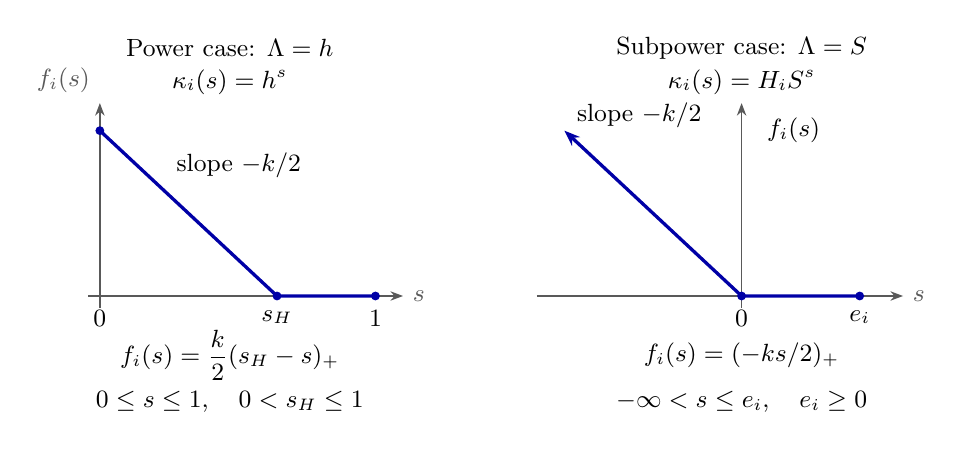
\begin{tikzpicture}[x=1cm,y=1cm,
  axis/.style={-{Stealth[length=1.6mm]},black!65,line width=.5pt},
  profile/.style={blue!65!black,line width=1.2pt},
  every node/.style={font=\small}]
 \begin{scope}
  \node at (1.65,3.15) {Power case: $\Lambda=h$};
  \node at (1.65,2.72) {$\kappa_i(s)=h^s$};
  \draw[axis] (-.15,0)--(3.85,0) node[right] {$s$};
  \draw[axis] (0,-.15)--(0,2.45) node[above left] {$f_i(s)$};
  \draw[profile] (0,2.1)--(2.25,0)--(3.5,0);
  \fill[blue!65!black] (0,2.1) circle (1.6pt)
                         (2.25,0) circle (1.6pt)
                         (3.5,0) circle (1.6pt);
  \node[below] at (0,-.06) {$0$};
  \node[below] at (2.25,-.06) {$s_H$};
  \node[below] at (3.5,-.06) {$1$};
  \node[above right] at (.85,1.38) {slope $-k/2$};
  \node at (1.65,-.75) {$f_i(s)=\dfrac{k}{2}(s_H-s)_+$};
  \node at (1.65,-1.35) {$0\le s\le1,\quad0<s_H\le1$};
 \end{scope}
 \begin{scope}[xshift=8.15cm]
  \node at (0,3.15) {Subpower case: $\Lambda=S$};
  \node at (0,2.72) {$\kappa_i(s)=H_iS^s$};
  \draw[axis] (-2.6,0)--(2.05,0) node[right] {$s$};
  \draw[axis] (0,-.15)--(0,2.45);
  \node[anchor=west] at (.2,2.1) {$f_i(s)$};
  \draw[profile,{Stealth[length=2mm]}-] (-2.25,2.1)--(0,0)--(1.5,0);
  \fill[blue!65!black] (0,0) circle (1.6pt)
                         (1.5,0) circle (1.6pt);
  \node[below] at (0,-.06) {$0$};
  \node[below] at (1.5,-.06) {$e_i$};
  \node at (-1.3,2.3) {slope $-k/2$};
  \node at (0,-.75) {$f_i(s)=(-ks/2)_+$};
  \node at (0,-1.35) {$-\infty<s\le e_i,\quad e_i\ge0$};
 \end{scope}
\end{tikzpicture}

 \caption{The forced amplitude-ratio profiles
 $r_{i,s}=\Lambda^{f_i(s)+o(1)}$. Their shapes follow from
 \Cref{f:profiles,f:binary,f:midpoint}, \eqref{f:power-end}, and
 \Cref{f:left-limit}. The panels show generic cases; the terminal
 flat segment may collapse at $s_H=1$ or $e_i=0$, respectively.
 The subpower domain continues to the left without a finite endpoint.
 The recomputed transition ratio is $\Lambda^{o(1)}$ in both cases,
 as used in the final incidence contradiction.}
 \label{f:profiles-figure}
\end{figure}

\subsection{The final incidence contradiction}

We finish the proof of Theorem~\ref{f:frame}. In the power case
\eqref{f:power-end} says that the recomputed transition ratio is
$\Lambda^{o(1)}$; in the subpower case the same assertion follows
from Lemma~\ref{f:left-limit}. The original transition masks have
remained fixed throughout.

One final occupancy deletion makes the use of packet tails
independent of any convergence rate for the profiles. Fix an
arbitrarily small $\eta>0$ and enlarge transition cells by
$\Lambda^\eta$ in their native coordinates. In the power case
count all visits. In the subpower case count points with
$e_b^2(z)\le CM_c\Lambda^{C_0\eta}$, where $C_0$ is sufficiently
large for polynomial weight comparison. This includes every
neighbor of a surviving original mask. The incident squares sum
to at most $\Lambda^{C_2\eta+o(1)}|Y|$. Since the transition ratio
is $\Lambda^{o(1)}$ and
$H_i^{k+2}A_i^{-q}=1$, the weighted $q$ charge of cells with more
than $\Lambda^{C_1'\eta}$ visits is at most
\[
 \Lambda^{(C_2-C_1')\eta+o(1)}D_i.
\]
Choose $C_1'>C_2$ sufficiently large. Lemma~\ref{f:selection}
propagates this error to the root with a negative power saving.
Do not reselect ratios after this deletion: all other transition
fields remain the same. The fixed packet decay, with the square
bound at surviving masks, makes tails outside the chosen radius
negligible relative to the high threshold. Thus each remaining
root point receives a substantial contribution from nearby
transition masks, each visited at most
$\Lambda^{C_1'\eta}$ times.

The field threshold is $A_i\Lambda^{-o(1)}=H_i^{k/2}\Lambda^{-o(1)}$.
At a root point the square sum of the transition backgrounds is
$\Lambda^{o(1)}$, and each transition amplitude is at most its
background times $\Lambda^{o(1)}$. Weighted Cauchy and bounded
absolute sums of the ancestor cutoffs therefore require at least
$H_i^k\Lambda^{-o(1)}$ nearby active masks. Letting the fixed
$\eta$ be arbitrarily small, double counting visits gives at least
\[
 |Y|H_i^k\Lambda^{-o(1)}
\]
distinct original transition masks.

Choose a field with $S_i=S$. Each of these masks had original
amplitude $a_T^{\mathrm{orig}}\ge cSH_i^{-k/2}$ in
\eqref{f:original-amplitudes}, and their original integrated square
budget is bounded by \eqref{f:original-energy}. Hence
\[
 D_i\gtrsim H_i^{k+2}
       \big(|Y|H_i^k\Lambda^{-o(1)}\big)
       \big(S^2H_i^{-k}\big)
 =|Y|H_i^{k+2}S^2\Lambda^{-o(1)}.
\]
This contradicts \eqref{f:hbalance} in the power case, because
$S$ is a fixed positive power of $\Lambda=h$, and contradicts
\eqref{f:subbalance} in the subpower case, because $S=\Lambda$.
The exact-packet estimate follows. Lemma~\ref{f:exact} transfers it
to compact profiles and fixes a finite derivative order after all
the fixed weight margins have been chosen. The countersequence
construction proves the uniform quantitative form
$C\delta^{-C}$ in \eqref{f:mainbound}, completing the proof.

\section{Fractal norms, compact arrays, and norm transport}
\label{d:section}

From this point the spatial dimension is $n\ge3$.  This section supplies
a weighted fractal estimate with an occupancy gain and a power saving
for frequency supports near affine $(n-2)$-planes.  In
Section~\ref{t:section}, these bounds will locate densely occupied
boxes and then permit pruning of the incident tube families so that
their direction laws do not concentrate near such planes.  We use
\begin{equation}
 \beta=\frac2{n+1},\qquad e=\frac{n^2}{n+1},
 \qquad \gamma_n=\frac{2n}{(n+1)(n+2)}.
 \label{d:exponents}
\end{equation}
The exponent $\beta$ is the measure homogeneity in the fractal square
norm.  Keeping that homogeneity explicit will distinguish a genuine
sparsity gain from a change of normalization.

\subsection{Arrays and measures}

\begin{definition}[Normalized compact arrays and admissible measures]
\label{d:measure}
A compact array of scale $L\ge1$ is a finite sum
\begin{equation}
 U(x,t)=\sum_\alpha c_\alpha L^{-n/2}
 e^{i(x\cdot\omega_\alpha-t|\omega_\alpha|^2)}
 \phi_\alpha\!\left(
     \frac{x-y_\alpha-2t\omega_\alpha}{L},\frac t{L^2}\right).
 \label{d:array}
\end{equation}
The frequencies $\omega_\alpha$ belong to a fixed bounded box.
The native profiles $\phi_\alpha$ are supported in a fixed box and have
uniform bounds for derivatives through a prescribed sufficiently large
finite order.  The number of labels
$(L\omega_\alpha,y_\alpha/L)$ in every unit phase-space ball is
bounded by a fixed constant.  Its coefficient energy is
$E(U)=\sum_\alpha|c_\alpha|^2$.
Subarrays retain their original profiles and labels.

A nonnegative Borel measure $\mu$ has $n$-dimensional growth with
parameter $m$ if
\begin{equation}
 \mu(B(z,r))\le m r^n\qquad(z\in\R^{n+1},\ r\ge1).
 \label{d:ball-growth}
\end{equation}
At array scale $L$ its native time range is bounded by a fixed
constant, so $\supp\mu\subset\{|t|\le C L^2\}$ after a common time
translation.  Fix a sufficiently large $M$.  The tube moment condition
with sparsity parameter $D$ is
\begin{equation}
 \int\left(1+
       \frac{|x-y_\alpha-2\omega_\alpha t|}{L}\right)^{-M}
          \dd\mu(x,t)
       \le \frac{mL^{n+1}}D
       \quad\text{for every included label }\alpha.
 \label{d:tube-moment}
\end{equation}
We use half-open unit cubes for all measure sums, so their masses add
without boundary ambiguity.
\end{definition}

To compare these conventions with \Cref{p:conventions}, set $k=n$
and $N=L$, and let $C_{\rm prof}$ be a fixed common bound for the
required native-profile derivatives. The choice
$s_\alpha=C_{\rm prof}L^{-n/2}|c_\alpha|$ is admissible, so the packet
energy parameter in \eqref{p:energy} is $C_{\rm prof}^2L^2E(U)$.
This is a normalization of packet sizes, not a spacetime
orthogonality assertion. The parameter $D$ in
\eqref{d:tube-moment} measures sparsity.

At any fixed bounded native time, transporting the intercepts along
their velocities preserves phase-space multiplicity: in the normalized
label variables it is a linear shear with bounded operator norm and
bounded inverse.  In particular,
\begin{equation}
 \norm{U}_\infty\le C E(U)^{1/2}.
 \label{d:array-sup}
\end{equation}
Indeed only $O(L^n)$ frequency/intercept labels can meet a point in the
fixed profile support; Cauchy--Schwarz cancels their square-root count
against $L^{-n/2}$.
Condition \eqref{d:tube-moment} with $D=1$ follows from
\eqref{d:ball-growth}, with fixed inflation of $m$.  To see this, on the
annulus of transverse radius $r=2^aL$, the bounded-time tube is covered
by $C(1+L^2/r)$ balls of radius $Cr$.  Its mass is at most
$Cm(r^n+L^2r^{n-1})$.  Multiplication by $2^{-aM}$ and summation over
$a\ge0$ give $CmL^{n+1}$ when $M$ is sufficiently large.

For later use, if labels lie in a frequency cube of side $H^{-1}$
centered at $v$, put
\begin{equation}
 X_{H,v}(x,t)=\left(\frac{x-2vt}{H},\frac t{H^2}\right).
 \label{d:parabolic-map}
\end{equation}
After removal of the common carrier, the field is
$H^{-n/2}U'(X_{H,v}(x,t))$, where $U'$ has scale $L/H$, frequency
$\omega'_\alpha=H(\omega_\alpha-v)$, intercept $y'_\alpha=y_\alpha/H$,
the same $c_\alpha$, and exactly the same native profile.  Thus native
regularity and normalized phase-space multiplicity are unchanged.

\subsection{The precise fractal input and its weighted form}

Write
\[
 \mathcal E g(x,t)=(2\pi)^{-n}
      \int e^{ix\cdot\xi-it|\xi|^2}g(\xi)\dd\xi,
\]
where $g\in L^2$ is supported in a fixed bounded frequency box.
Fixed changes of that box alter constants only.

\begin{theorem}[Du--Zhang input in squared form]
\label{d:dz-input}
Let $\mathcal Q$ be a collection of distinct unit lattice cubes in a
ball of radius $S\ge1$.  Suppose their counting function in every ball
of radius $r\ge1$ is at most $\Gamma r^n$, and their number in any ball
of radius $\sqrt S$ is at most $\lambda_0$.  Then for every $\eps>0$,
\begin{equation}
 \sum_{q\in\mathcal Q}\sup_q|\mathcal E g|^2
 \le C_\eps S^{\eps}
       \Gamma^{4/((n+1)(n+2))}\lambda_0^{\gamma_n}
       S^{\gamma_n}\norm{g}_2^2.
 \label{d:dz-sup}
\end{equation}
All fixed enlargements and translations of the cube lattice are
allowed, with fixed changes of the constant.
\end{theorem}

\begin{proof}
The exact external input is \citet[Theorem~1.6]{DuZhang2019} with counting
exponent $n$.  On a union $X$ of unit cubes for which every occupied
$\sqrt S$ lattice parent has comparable occupancy $\lambda$, it states
\[
 \norm{\mathcal E g}_{L^2(X)}
 \le C_\eps\Gamma^{2/((n+1)(n+2))}
       \lambda^{n/((n+1)(n+2))}
       S^{n/((n+1)(n+2))+\eps}\norm{g}_2.
\]
The original unit-ball frequency hypothesis is changed to our fixed
box by a fixed parabolic dilation and bounded coverings.  The same
holds for balls with arbitrary centers by translating the extension,
which only modulates its input.  Squaring and renaming $\eps$ gives
the exponents in \eqref{d:dz-sup} for an integral over $X$.
No comparable-field-norm assumption occurs in this theorem; that
additional hypothesis belongs to Proposition~3.1 of the cited paper,
which is not needed here.

Choose a comparable ambient scale with a compatible square-root grid.
Group whole square-root parents according to their dyadic occupancy.
A parent is covered by boundedly many radius-$\sqrt S$ balls, so its
occupancy is at most $C\lambda_0$.  Each group inherits the counting
bound.  Sum the squared theorem over these groups; the resulting series
$\sum_{2^a\le C\lambda_0}2^{a\gamma_n}$ is bounded by
$C\lambda_0^{\gamma_n}$.  This removes the equal-occupancy hypothesis.

Finally, $\mathcal E g$ has spacetime Fourier support in a fixed compact
paraboloid patch.  Choose a Schwartz reproducing kernel equal to one
on that patch in Fourier space.  Cauchy--Schwarz and local boundedness
of translates of this kernel imply, for every sufficiently large $A$,
\[
 \sup_q|\mathcal E g|^2
 \le C_A\int_{\R^{n+1}}(1+|h|)^{-A}
            \int_q|\mathcal E g(z+h)|^2\dd z\dd h.
\]
For each fixed $h$, the translated field is an exact extension of an
input of the same norm and support.  Apply the integral estimate on
the unchanged cube collection, then integrate in $h$.  This proves
\eqref{d:dz-sup} without enlarging the ambient radius for distant
translations.
\end{proof}

\begin{proposition}[Weighted fractal norm and occupancy gain]
\label{d:fractal}
\label{d:refined}
Suppose $\mu$ is supported in a ball of radius $CS$, satisfies
\eqref{d:ball-growth}, and, in addition,
\begin{equation}
 \mu(B(z,\sqrt S))\le d\,m S^{n/2},
 \qquad S^{-A_0}\le d\le1.
 \label{d:sqrt-occupancy}
\end{equation}
Then
\begin{equation}
 \sum_q\mu(q)^\beta\sup_q|\mathcal E g|^2
 \le C_{\eps,A_0}\,m^\beta
       S^{n/(n+1)+\eps}d^{\gamma_n}\norm{g}_2^2.
 \label{d:weighted-fractal}
\end{equation}
With $d=1$ no extra assumption beyond growth is needed.  The estimate
is homogeneous in $\mu$ and in the squared input norm.
\end{proposition}

\begin{proof}
Normalize $m=\norm{g}_2=1$; zero cases are immediate.  Sort unit cubes
by $a<\mu(q)\le2a$, where $a$ runs over a fixed multiple of the
nonpositive dyadic powers.  Cubes meeting a radius-$r$ ball lie in a
fixed enlargement, and their disjoint masses are at least $a$ times
their number.  Thus this class has counting parameter at most $Ca^{-1}$
and square-root occupancy at most $CdS^{n/2}a^{-1}$.  Applying
\Cref{d:dz-input} and multiplying by $(2a)^\beta$ gives
\begin{align*}
 \sum_{a<\mu(q)\le2a}\mu(q)^\beta\sup_q|\mathcal E g|^2
 &\le C_\eps S^\eps a^\beta
       (a^{-1})^{4/((n+1)(n+2))}
       (dS^{n/2}a^{-1})^{\gamma_n}S^{\gamma_n}\\
 &=C_\eps S^{n/(n+1)+\eps}d^{\gamma_n}.
\end{align*}
The two cancellations are
\[
 \beta-\frac4{(n+1)(n+2)}-\gamma_n=0,
 \qquad (1+n/2)\gamma_n=\frac n{n+1}.
\]
This exact cancellation leaves no positive power of $a$ to sum, so a
small-mass truncation is necessary.  Bounded frequency support gives
$\norm{\mathcal E g}_\infty\le C$, and there are $O(S^{n+1})$ relevant
unit cubes.  Those with $\mu(q)\le S^{-A}$ contribute at most
$CS^{n+1-A\beta}$.  Choose $A$ so large, in terms of $A_0$ and a
prescribed error power, that this is bounded by
$S^{-B}d^{\gamma_n}$.  There remain $O_A(1+\log S)$ mass classes.
Use half the requested loss in the preceding class estimate and absorb
this count into the remaining $S^\eps$.  Restoring homogeneity proves
\eqref{d:weighted-fractal}.
\end{proof}

\subsection{Exact Fourier layers and spatial localization}

The following reduction permits compact native profiles in estimates
that tolerate an arbitrarily small power loss.  Its common frequency
shift is useful when the chosen subarray changes from one test to
another.

\begin{lemma}[Exact Fourier layers of compact profiles]
\label{d:layers}
For every prescribed finite collection of derivative and native spatial
decay orders, a sufficiently high finite profile regularity in
\eqref{d:array} gives a representation
\begin{equation}
 U(x,t)=\sum_{k\in\Z^n}\int_\R
       \rho(k,u)e^{iu t/L^2}\mathcal E g_{k,u}(x,t)\dd u,
 \label{d:layer-representation}
\end{equation}
where $\rho(k,u)\le C_A(1+|k|+|u|)^{-A}$ for any prescribed $A$.
For every subarray $\mathcal A$,
\begin{equation}
 \norm{g_{k,u}^{\mathcal A}}_2^2
       \le C\sum_{\alpha\in\mathcal A}|c_\alpha|^2.
 \label{d:layer-subarray-energy}
\end{equation}
Each label contributes an exact input supported within $O(L^{-1})$ of
$\omega_\alpha+k/L$, with uniformly bounded native frequency
seminorms.  On a fixed native time range, its extension has all the
prescribed spatial decay about the original trajectory after the
factor $\rho$ is extracted.  The shift $k/L$ and the time modulation
are common to the entire layer and every subarray.  For any fixed
$\eta>0$, the portion $|k|>L^\eta$ can be made an arbitrarily negative
power error in the array supremum, and hence in tests involving
polynomially many cubes and polynomially bounded mass parameters.
\end{lemma}

\begin{proof}
Fourier transform $\phi_\alpha$ in its native variables, denoting the
dual variables by $(\eta,\zeta)$.  Insert a smooth bounded-overlap
partition $\sum_k\vartheta_k(\eta)=1$ into bounded boxes about
$k\in\Z^n$, and change variables $u=\zeta+|\eta|^2$.
For fixed $(k,u)$ define the input, in $\xi=\omega_\alpha+\eta/L$
coordinates, by
\[
 g_{\alpha,k,u}(\omega_\alpha+\eta/L)
   =C c_\alpha L^{n/2}e^{-iy_\alpha\cdot\eta/L}
       \vartheta_k(\eta)
       \widehat\phi_\alpha(\eta,u-|\eta|^2).
\]
Fourier inversion gives
\[
 U=\sum_k\int e^{iu t/L^2}
                     \mathcal E\Big(\sum_\alpha g_{\alpha,k,u}\Big)
                     \dd u.
\]
Compact support and sufficiently many derivatives of $\phi_\alpha$
give any prescribed polynomial decay in $(\eta,\zeta)$, also after a
fixed number of frequency derivatives.  The change
$\zeta=u-|\eta|^2$ costs only polynomial factors.  Extract
$\rho(k,u)=C_A(1+|k|+|u|)^{-A}$ with $C_A$ chosen to bound the needed
seminorms, and put the remaining normalized sum into $g_{k,u}$.
Increasing the finite initial derivative order supplies these bounds
simultaneously.

The input norm estimate follows by a summable Gram-matrix bound.
Two normalized input bumps can interact only if
$|L(\omega_\alpha-\omega_{\alpha'})|\le C$, since the shift $k$ is
common.  For these pairs, integration by parts in the native frequency
variable gives any prescribed decay in
$|y_\alpha-y_{\alpha'}|/L$.  The coefficient factors are
$c_\alpha\overline{c_{\alpha'}}$ and all remaining seminorms are
uniform.  Phase-space counting therefore bounds the absolute row and
column sums of the Gram matrix.  Schur's inequality proves
\eqref{d:layer-subarray-energy}, without requiring the subarray to be a
Fourier projection.

For spatial decay, the phase in native variables is
$z\cdot\eta-\tau|\eta|^2$.  On bounded $\tau$ and $\eta$ near $k$,
integration by parts gives rapid decay in $z$ away from the original
trajectory, at the cost of a fixed polynomial in $k$.  This was
included in the orders used to extract $\rho$; derivatives of the
extension are handled at the same time.  The common shift preserves
all relative frequency labels and phase-space counts.
Finally, Cauchy--Schwarz over labels and the prescribed rapid spatial
decay bound every normalized layer by a fixed polynomial in $(k,u)$
times $E(U)^{1/2}$.  Increase $A$, sum over $|k|>L^\eta$, and integrate
in $u$ to obtain $C_B L^{-B}E(U)^{1/2}$ for any required $B$.
All orders here are fixed before the varying scale $L$.
\end{proof}

\begin{lemma}[Exact packet localization on a time slab]
\label{d:packet-expansion}
Let $T\ge1$ and let $g$ have bounded frequency support.  On a time
interval of length $O(T)$, an exact extension can be localized to
spatial boxes of side $T$ with summed input energies
$C\norm{g}_2^2$.  The localization errors have arbitrarily high negative
powers of $T$, with summable local squared budgets.  No factor equal
to the number of spatial boxes is needed.
\end{lemma}

\begin{proof}
Set $R=\sqrt T$ and absorb the initial time into the input by a
unit-modulus multiplier.  Partition frequency into $R^{-1}$ caps and
expand each rescaled cap density in a Fourier series on a fixed larger
box.  With smooth bumps equal to one on the cap supports, this gives
exact packets
\[
 c_{\theta,m}R^{-n/2}e^{i(x\cdot\omega_\theta-t|\omega_\theta|^2)}
 H_\theta\!\left(
     \frac{x-\gamma Rm-2t\omega_\theta}{R},\frac t{R^2}\right),
 \qquad \sum_{\theta,m}|c_{\theta,m}|^2\le C\norm{g}_2^2.
\]
Here $H_\theta$ is the extension of a fixed smooth native frequency
bump.  It and any fixed derivatives decay arbitrarily rapidly in the
first variable for bounded second variable.  Parseval proves the
coefficient bound; differentiating the input density is unnecessary.
The same cap-overlap and integration-by-parts Gram bound used in
\Cref{d:layers} bounds the squared norm of any retained exact input by
its coefficient energy.

For a spatial box $B$ of side $T$, retain packets whose trajectories
on the time slab come within $CT$ of $B$.  A bounded-velocity
trajectory of duration $O(T)$ can be retained for only $O(1)$ such
boxes.  Therefore these retained energies sum to
$C\norm{g}_2^2$.  For the omitted packets, the native distance from the
box is at least $c\sqrt T$.  Extract an arbitrary negative power of
$T$ from the rapid packet decay and keep a further weight in the
distance from the trajectory to $B$, measured in units of $T$.
Cauchy--Schwarz and phase-space counting bound the squared supremum of
the omitted field on $B$ by
\[
 C_A T^{-A}\sum_{\theta,m}|c_{\theta,m}|^2
       \left(1+\frac{\dist(B,\text{trajectory}_{\theta,m})}{T}
       \right)^{-n-2}.
\]
The right-hand budgets sum boundedly in $B$.  This proves the asserted
error control and also permits arbitrarily long spatial unions of
such boxes.  Translations modulate the exact inputs and preserve their
norms, so the construction is uniform in the slab and box centers.
\end{proof}

\begin{corollary}[Power-loss norm for compact arrays]
\label{d:power-loss}
Let $U$ be a compact array of scale $L$, and let $\mu$ satisfy
\eqref{d:ball-growth} in a spacetime box of side $O(L^2)$.
For every $\eps>0$, with sufficiently many fixed profile derivatives,
\begin{equation}
 \sum_q\mu(q)^\beta\sup_q|U|^2
       \le C_\eps m^\beta L^{2n/(n+1)+\eps}E(U).
 \label{d:compact-fractal}
\end{equation}
\end{corollary}

\begin{proof}
Apply \Cref{d:layers}, discarding $|k|>L^\eta$ with a sufficiently high
negative power.  For $0<\eta<1$, every retained layer has support in a
fixed bounded frequency box.  Apply \Cref{d:fractal} with $S=L^2$ and
$d=1$ to each exact layer.  Minkowski's inequality for the weighted
$\ell^2$ norm of unit-cube suprema, followed by
\eqref{d:layer-subarray-energy}, gives the result because
$\sum_k\int\rho(k,u)\dd u<\infty$.  The common time modulation has
absolute value one.  The discarded error is negligible: each cube
has mass at most $Cm$, there are $O(L^{2(n+1)})$ relevant cubes, and
its supremum has any required negative power of $L$.  Rename the
arbitrarily small scale loss after replacing $S$ by $L^2$.
\end{proof}

\subsection{Coarse decoupling and exact transport powers}

For dyadic $K\ge2$, $0<b<1$, and $P=2/(1-b)$, define
\begin{equation}
 \mathcal T_b(V,\nu)
       =\sum_{Q\in\mathcal Q_{K^2}}
              \nu(Q)^b\norm{V}_{L^P(Q)}^2,
 \label{d:coarse-functional}
\end{equation}
where $\mathcal Q_{K^2}$ is a fixed grid of half-open spacetime cubes
of side $K^2$.

\begin{lemma}[Decoupling inside a strip]
\label{d:strip-decoupling}
Group a field $V=\sum_\theta V_\theta$ by frequency-label bins of side
$K^{-1}$.  Suppose the field supports lie in fixed enlargements of
these bins and within vertical Fourier distance $O(K^{-2})$ of the
paraboloid.  If the labels lie within $O(K^{-1})$ of an affine
$j$-plane, $1\le j\le n$, and $2\le P\le q_j=2(j+2)/j$, then
\begin{equation}
 \norm{V}_{L^P(Q)}^2
 \le C_{\eps,A}K^\eps
       \sum_\theta\sum_{a\in\Z^{n+1}}\braket{a}^{-A}
                 \norm{V_\theta}_{L^P(Q+K^2a)}^2.
 \label{d:local-strip-decoupling}
\end{equation}
The constituent fields may be arbitrary prescribed subfields with
these supports.  Without the strip hypothesis the same estimate holds
with the factor $CK^n$ in place of $C_\eps K^\eps$.
\end{lemma}

\begin{proof}
Rotate frequency into tangent and normal coordinates for the affine
plane, remove its central normal carrier, and shear away the normal
linear time phase.  The remaining normal frequencies have size
$O(K^{-1})$, so their quadratic contribution is $O(K^{-2})$.
On each fixed normal physical slice, the tangential spacetime Fourier
support is therefore within $O(K^{-2})$ of the positive $j$-dimensional
paraboloid.  Multiply first by a Schwartz cutoff bounded below on $Q$
with Fourier width $O(K^{-2})$.  It preserves this support statement
with fixed enlargement.

Apply paraboloid decoupling \citep{BD2015} in the range $P\le q_j$.
After this localization, use smooth tangential cap projections; their
spatial convolution kernels have bounded $L^1$ norm.  Only boundedly
many original enlarged grid bins in the strip can meet a projected
bin, since both the normal thickness and tangential cap size are
$O(K^{-1})$.  Bounded overlap and Minkowski in the normal physical
variables give the squared-norm estimate with a Schwartz weight
outside $Q$.  Decomposing that weight into translates of $Q$ gives
\eqref{d:local-strip-decoupling}, with any fixed $A$.
This proof uses only supports and not the way a subfield was selected.
Without a strip, there are $O(K^n)$ bins, and Cauchy--Schwarz gives the
stated alternative directly.
\end{proof}

\begin{lemma}[Coarse norm transport]
\label{d:transport}
Let $F=X_{K,v}$ with bounded $v$, and suppose
$V(z)=K^{-n/2}e^{i\varphi(z)}V'(Fz)$ with $|e^{i\varphi}|=1$.
For a fixed $a\in\Z^{n+1}$,
\begin{equation}
 \sum_Q\nu(Q)^b\norm{V}_{L^P(Q+K^2a)}^2
 \le C K^{2-(n+2)b}\sum_{r,s\in\mathcal R}
                 \mathcal T_b(V',\nu_{a,r,s}),
 \label{d:transport-functional}
\end{equation}
where $\mathcal R$ is a fixed finite set, independent of $Q,K,a$, and
\begin{equation}
 \nu_{a,r,s}
  =(\tau_{F(K^2a)+K^2(s-r)})_\# F_\#\nu,
 \qquad \tau_h(z)=z+h.
 \label{d:translated-measures}
\end{equation}
Their translations have size at most $CK^2(1+|a|)$.  The same conclusion
holds with any prescribed subset of parent cubes on the left.
If $\nu$ has growth parameter $m$, each child measure has parameter
$CmK^{n+1}$.  Direct pushforward transports
\eqref{d:tube-moment} from scale $L$ to $L/K$ with the same $D$.
\end{lemma}

\begin{proof}
The Jacobian of $F$ is $K^{-(n+2)}$.  Thus, with
$A_Q=F(Q+K^2a)$,
\begin{align*}
 \norm{V}_{L^P(Q+K^2a)}^2
 &=K^{-n+2(n+2)/P}
          \left(\int_{A_Q}|V'|^P\right)^{2/P}\\
 &=K^{2-(n+2)b}
          \left(\int_{A_Q}|V'|^P\right)^{1-b}.
\end{align*}
No density factor accompanies the mass: the measure is the direct
pushforward.  Let $\nu_a=(\tau_{F(K^2a)})_\#F_\#\nu$.
Then $\nu_a(A_Q)=\nu(Q)$, and the $A_Q$ are disjoint.
Group them according to the child $K^2$ cube $C$ containing their
centers.  Each $A_Q$ has diameter $O(K)$, so all sets in a group are
contained in
$C^*=\bigcup_{r\in\mathcal R}(C+K^2r)$ for a fixed finite
$\mathcal R$.  Hölder with exponents $1/b$ and $1/(1-b)$ gives
\[
 \sum_{Q\text{ in the group}}\nu(Q)^b
          \left(\int_{A_Q}|V'|^P\right)^{1-b}
 \le \nu_a(C^*)^b\norm{V'}_{L^P(C^*)}^2.
\]
Subadditivity of the powers $b$ and $1-b$ bounds this by
\[
 \sum_{r,s\in\mathcal R}\nu_a(C+K^2r)^b
                      \norm{V'}_{L^P(C+K^2s)}^2.
\]
The two indices allow the mass and the field norm to occupy different
neighbors.  Reindex by $D=C+K^2s$ to obtain precisely
\eqref{d:translated-measures} and
\eqref{d:transport-functional}.  None of the translations depends on
which parent cube was selected.

The inverse image of a radius-$r$ ball under $F$ has $n$ transverse
widths $O(Kr)$ and longitudinal length $O(K^2r)$.  It is covered by
$O(K)$ balls of radius $CKr$.  Hence its mass is at most
$CmK^{n+1}r^n$ for $r\ge1$, and translations preserve this bound.
For the tube moment, writing $L'=L/K$,
$\omega'=K(\omega-v)$, and $y'=y/K$ gives the identity
\[
 \frac{x'-y'-2\omega't'}{L'}
       =\frac{x-y-2\omega t}{L},
 \qquad (mK^{n+1})(L/K)^{n+1}=mL^{n+1}.
\]
This proves the direct-pushforward assertion.  When the tube centers
are kept fixed, translated measures preserve the moment up to a fixed
factor only if their native displacements are bounded.  Accordingly,
applications requiring this moment truncate the Schwartz shifts while
the child packet widths are much larger than the retained shifts.
The freely chosen exponent $A$ in
\eqref{d:local-strip-decoupling} makes the omitted tail smaller than
any prescribed power once the global suprema and occupied cube counts
are polynomially bounded.  For exact-field applications using only
ball growth, arbitrary translations are harmless.
\end{proof}

\subsection{A power gain from codimension two}

\begin{proposition}[Codimension-two strip saving]
\label{d:strip}
Fix $0<\alpha<1/8$.  Suppose $g$ has bounded frequency support contained
in an $O(S^{-\alpha})$ neighborhood of an affine $(n-2)$-plane, and
$\mathcal Q$ is a collection of unit cubes in a ball of radius $S$ with
at most $m_0r^n$ cubes in every radius-$r$ ball, $r\ge1$.
Fix any $b$ with $\beta<b<2/n$.
There is $c_0>0$, depending only on the fixed dimensional choices and
independent of $\alpha$, such that for every $\eps>0$,
\begin{equation}
 \sum_{q\in\mathcal Q}\sup_q|\mathcal E g|^2
 \le C_{\alpha,\eps}m_0^b
           S^{n/(n+1)-c_0\alpha+\eps}\norm{g}_2^2.
 \label{d:strip-saving}
\end{equation}
In particular, for $m_0=S^{o(1)}$ this is the saving
$S^{n/(n+1)-c_0\alpha+o(1)}$.  Finite disjoint subinputs are allowed,
with their squared norms summed on the right.
\end{proposition}

\begin{proof}
Choose a sufficiently large integer $J$, fixed independently of $S$
and $\alpha$, and dyadic $K$ so that
$H=K^J\asymp S^\alpha$, with fixed rounding factors.
Set $P=2/(1-b)$.  Since $b<2/n$, one has
$P<q_{n-2}=2n/(n-2)$.
Use the counting measure of the selected unit cubes, assigning unit
mass to their centers.  Local constancy and Hölder bound the initial
sum of squared suprema by the coarse functional
\eqref{d:coarse-functional}, with a fixed $K^C$ endpoint cost allowed.
Explicitly, in each coarse cube the sum of the local unit norms is
bounded by the number of selected unit cubes to the power
$1-2/P=b$, times the squared $L^P$ norm on a fixed enlargement.
Schwartz reproduction supplies the required neighboring translates.
Its measure parameter is $Cm_0$.

Iterate \Cref{d:strip-decoupling,d:transport} for $J$ levels.
After $a$ rescalings the strip width is $O(K^a/H)$, which is at most
$O(K^{-1})$ before the last step.  Thus the codimension-two decoupling
hypothesis persists.  The product of transport factors is
$H^{2-(n+2)b}$, up to constants depending on the fixed $J$, while the
final measure parameter is
\[
 m'\le C_Jm_0H^{n+1}.
\]
Smooth frequency decompositions have bounded overlap, so final child
input squared norms sum to $C_J\norm{g}_2^2$.
The $J$ decoupling losses can be made $S^\eps$ by starting with a
sufficiently small loss.  Schwartz shifts may be truncated at a
polynomial radius with negligible error, using bounded-frequency
suprema and polynomial cube counts.  Their weight sums cost fixed
constants at each of the fixed number of levels.

The final time length is
$T=S/H^2$, still a fixed positive power of $S$.
The spatial region can have side $S/H$; to avoid paying for this
aspect ratio, cover it by spatial boxes of side $T$ and use
\Cref{d:packet-expansion} on the child time slab.  Retained exact inputs
have squared norms summable to the child energy.  Their omitted
errors have arbitrarily high negative powers of $T$, with summable
local budgets.  Each resulting spacetime box has side $O(T)$.

Here is the terminal coarse-functional estimate on one such box:
\begin{equation}
 \mathcal T_b(V',\nu')
 \le C_\eps K^{C_*}T^{n/(n+1)+\eps}(m')^b
                      \norm{\text{child input}}_2^2.
 \label{d:terminal-functional}
\end{equation}
Its exponent $C_*$ is independent of $J$.  Indeed, replace the field
norm on each $K^2$ cube by its volume factor times a unit-cube witness
for its supremum.  Move the entire mass of that coarse cube to that
witness.  The resulting measure has ball parameter at most
$CK^{2n}m'$, and each moved mass is at most $CK^{2n}m'$.
Since $b\ge\beta$, its $b$th power is at most
$(CK^{2n}m')^{b-\beta}$ times its $\beta$th power.
Apply \Cref{d:fractal} at scale $T$ to the moved masses.  The volume
factor, the moved growth parameter, and this last comparison produce
only $K^{C_*}$, proving \eqref{d:terminal-functional}.
A bounded number of witness-grid choices and enlargements have the
same cost.  The inequality holds separately for every translated
child measure, and translations are absorbed into modulations of the
exact inputs.  Consequently no count of spatial boxes or translation
labels is introduced.

Combining the three scale contributions, apart from
$S^{n/(n+1)+\eps}$ and the fixed endpoint factor $K^{C_*}$, gives
\begin{align*}
 H^{2-(n+2)b}\,H^{(n+1)b}\,H^{-2n/(n+1)}
   &=H^{2-b-2n/(n+1)}\\
   &=H^{\beta-b}.
\end{align*}
Enlarge $C_*$ to include the initial endpoint cost, still independently
of $J$.  Choose $J$ so large that
$C_*/J<(b-\beta)/2$.  Then
$K^{C_*}H^{\beta-b}\le H^{-(b-\beta)/2}$.
Taking, for example, any $c_0<(b-\beta)/2$ absorbs the fixed rounding
and proves \eqref{d:strip-saving}.  Constants may depend on fixed
$\alpha,J,\eps$, but the saving exponent $c_0$ does not depend on
$\alpha$.  For disjoint subinputs the same construction is applied
with their coefficient energies, whose sum is the original energy.
\end{proof}

\section{A transverse saving in every fixed dimension}
\label{t:section}

Throughout this section the spatial dimension $n\ge3$ is fixed, and
\[
 \beta=\frac{2}{n+1},\qquad e=\frac{n^2}{n+1}.
\]
For a frequency $\xi$ write $v(\xi)=(2\xi,1)$; replacing these
vectors by unit vectors changes determinants by bounded factors on
a fixed bounded frequency region.  We write $Ef=\mathcal E f$ for the
exact extension operator of Section~\ref{d:section}.  The following statement concerns
exact extension fields.  Its use for smooth packet arrays will come
after the exact Fourier-layer reduction in the next section.

\begin{proposition}[Transverse saving]\label{t:transverse}
Fix a bounded frequency region in $\R^n$.  There are $c>0$ and
$L_0<\infty$, depending only on this region and $n$, such that the
following configuration is impossible for $L\ge L_0$.  Let
$\mathcal Q$ be distinct unit lattice cubes in a ball of radius $L^2$
in $\R^{n+1}$, with
\begin{equation}\label{t:forbidden-counts}
 \#\mathcal Q\ge L^{2n-c},\qquad
 \#\{q\in\mathcal Q:q\cap B(z,r)\ne\varnothing\}
       \le L^c r^n\quad(r\ge1).
\end{equation}
Suppose $f_1,\ldots,f_{n+1}$ have $L^2$ norm at most one, frequency
support in the fixed region, and
\[
 \sup_q|Ef_i|\ge L^{-e-c}
       \quad(q\in\mathcal Q,\ 1\le i\le n+1).
\]
It is impossible that every choice of one frequency from each support
has direction determinant at least $L^{-c}$ in absolute value.
\end{proposition}

We prove the equivalent assertion that no countersequence exists with
$c\downarrow0$ and $L\to\infty$.  In this section $o(1)$ refers to
such a sequence, after subsequences when necessary.  Estimates available
with every fixed positive power loss may be diagonalized to have
$L^{o(1)}$ loss.  The constants in each such estimate are fixed before
diagonalization.  The proof uses the limiting information calculus of
\citet[Section~3, ``Limiting information calculus'']{PSE2026}.  We state
the usable facts below and prove the changes needed in dimension $n$.
In particular, the planar transverse proposition in that source is not
used as a higher-dimensional assertion.

\subsection{Uniform multilinear estimates and incident weights}

We first specify the dependence on transversality.  This prevents a
subpower determinant loss from concealing an uncontrolled constant.

\begin{lemma}[Multilinear estimates with polynomial dependence]
\label{t:multilinear}
If $n+1$ bounded-frequency exact inputs are transverse with determinant
at least $\nu\in(0,1]$, then, for each $\eps>0$,
\begin{equation}\label{t:multilinear-extension}
 \sum_{q\subset B_S}\prod_{i=1}^{n+1}
       \bigl(\sup_q|Ef_i|\bigr)^{2/n}
 \le C_\eps\nu^{-M_\eps}S^\eps
                    \prod_{i=1}^{n+1}\norm{f_i}_2^{2/n}.
\end{equation}
The same bound holds with the sum replaced by the integral of the
product.  For transverse families of tubes of width $\delta$ in a fixed
bounded region, with nonnegative weights $w_i(T)$, the corresponding
Kakeya bound is
\begin{equation}\label{t:kakeya}
 \int\prod_{i=1}^{n+1}
       \left(\sum_Tw_i(T)\mathbf1_T\right)^{1/n}
 \le C_\eps\nu^{-M_\eps}\delta^{n+1-\eps}
             \prod_i\left(\sum_Tw_i(T)\right)^{1/n}.
\end{equation}
Fixed enlargements are allowed.  Subpower enlargements and
$\nu=S^{-o(1)}$ give only subpower losses.
\end{lemma}

\begin{proof}
Subdivide direction supports into neighborhoods of radius a sufficiently
small fixed power of $\nu$.  There are $\nu^{-O_n(1)}$ choices of
$(n+1)$ neighborhoods.  For each choice, send representative directions
to the coordinate axes.  The map, its inverse, and its determinant have
size bounded by fixed powers of $\nu^{-1}$.  The near-coordinate-axes
multilinear Kakeya theorem
\citep[Theorem~1.15 and Remark~1.10]{BCT2006}, or its strengthened form
\citep{Guth2010}, gives \eqref{t:kakeya} after summing the choices.
Weights follow by repetition and approximation.

Here is the finite induction giving the required uniform restriction
constant.  Let $A_B(S,\nu)$ be the best normalized integral constant
for inputs in a fixed box of size $B$.  Decompose each input into exact
packets at radius $S$, and on each $\sqrt S$-box retain the packets
meeting its $S^\theta\sqrt S$ enlargement.  Their input squared norms
are bounded by incident coefficient energy, and the discarded fields
are $O_N(S^{-N})$ relative to their parent input norms.  The enlarged
supports remain $\nu/2$ transverse if $S^{-1/2}\le c_B\nu$.
After rescaling by $S$, the padded tubes have width
$\delta=S^{-1/2+\theta}$.  Apply \eqref{t:kakeya} with loss $\sigma$.
Dividing its bound by the volume $S^{-(n+1)/2}$ of a rescaled
$\sqrt S$-box gives
\[
 A_B(S,\nu)\le C\nu^{-M_\sigma}S^a
          A_{B+1}(C_B\sqrt S,\nu/2)+O_N(S^{-N}),
 \qquad a=(n+1)\theta+\sigma/2.
\]
Increasing $N$ absorbs all errors into the same inequality for $1+A_B$;
when expanding products with exponent $2/n\le1$, use subadditivity to
bound terms containing a discarded factor.  For a prescribed $\eps$,
choose a finite $J$ with $(n+1)2^{-J}<\eps/2$, and then $\theta,\sigma$
with $2a<\eps/2$.  Iterating $J$ times and using the terminal trivial
bound $O(S_J^{n+1})$, where $S_J\asymp S^{2^{-J}}$, proves the
integral estimate when $S\ge(C/\nu)^{2^J}$.  In the complementary
range the trivial bound is absorbed by increasing $M_\eps$.
Thus the dependence on $\nu^{-1}$ is a fixed power.

For the cube-supremum version the exponent $p=2/n$ can be below one,
so we include the submean argument.  If $F$ has Fourier support in the
fixed compact region, choose a Schwartz reproducing kernel $\psi$ and
write $F=\psi*F$.  For $A>0$ let
$M_AF(x)=\sup_y|F(x-y)|(1+|y|)^{-A}$, which is finite because these
extensions are bounded.  In the convolution insert
$|F(w)|\le|F(w)|^p M_AF(x)^{1-p}(1+|x-w|)^{A(1-p)}$.
Peetre's elementary inequality
$(1+|x-w|)\le(1+|x-z|)(1+|z-w|)$ then gives, uniformly in $z$,
\[
 \frac{|F(z)|}{(1+|x-z|)^A}
 \le C_A M_AF(x)^{1-p}
             \int(1+|x-w|)^{-Ap}|F(w)|^p\dd w,
\]
using the boundedness of $(1+|z-w|)^A|\psi(z-w)|$.
Taking the supremum and dividing by $M_AF(x)^{1-p}$ proves the
required Schwartz-average bound for $M_AF(x)^p$; the zero case is
immediate.  Choose $Ap$ arbitrarily large.  In particular this bounds
$(\sup_q|Ef_i|)^{2/n}$ by that average for each $x\in q$.
Integrate the product over $q$ and sum.  For each independent list of
shifts the translated fields are exact extensions with unchanged norms
and supports.  Apply the integral estimate and integrate the Schwartz
weights.  This proves \eqref{t:multilinear-extension}.
\end{proof}

\begin{lemma}[Pruned incident-tube model]\label{t:tubes}
A countersequence to Proposition~\ref{t:transverse} yields a set
$\mathcal P$ of centers of distinct $L^{-1}$-scale cubes in a bounded
region, satisfying
\begin{equation}\label{t:point-counts}
 \#\mathcal P=L^{n+o(1)},\qquad
 \#(\mathcal P\cap B(z,r))\le L^{n+o(1)}r^n
                     \quad(L^{-1}\le r\le1),
\end{equation}
and $n+1$ transverse weighted tube families of width $L^{-1+o(1)}$.
Their weights satisfy $\sum_Tw_i(T)\lesssim1$.  For every $x\in\mathcal P$
there is an incident subfamily of retained weight
$w_i^*(x)=L^{-e+o(1)}$ whose normalized law satisfies
\begin{equation}\label{t:strip-law}
 \mathbb P\{\xi(T_i)\in N_{L^{-\alpha}}(H)\mid X=x\}
       \le L^{-c_1\alpha+o(1)}
\end{equation}
for every affine $(n-2)$-plane $H\subset\R^n$ and every fixed rational
$0<\alpha<1/8$.  Here $c_1>0$ is fixed independently of $\alpha$, and
the estimate is uniform in $x,H$ for each fixed $\alpha$.
\end{lemma}

\begin{proof}
Sort the original unit cubes by their occupancy in $L$-boxes.  A dyadic
class retains $L^{2n-o(1)}$ cubes, on which the squared supremum sum of
each field is at least $L^{2n-2e-o(1)}=L^{2n/(n+1)-o(1)}$.
The refined fractal estimate, Proposition~\ref{d:refined}, at radius
$L^2$ improves this upper bound by a fixed power if the $L$-box
occupancy is at most $L^{n-\delta}$ for any fixed $\delta>0$.
The counting hypothesis supplies the upper bound $L^{n+o(1)}$.
Consequently the retained occupancies are $L^{n+o(1)}$.
Divide coordinates by $L^2$ and use the occupied box centers.  Counting
the original cubes in an enlarged ball, then dividing by the minimum
occupancy, proves \eqref{t:point-counts}.

Exact packet localization at radius $L^2$ gives coefficient weights with
bounded total sum.  On each retained physical $L$-box, keep trajectories
in a padded enlargement.  The padding exponent can tend sufficiently
slowly to zero; rapid tails make the discarded field negligible.
The retained exact input has squared norm at most $Cw_i(x)$, where
$w_i(x)$ is its incident weight.  Apply Proposition~\ref{d:fractal}
at radius $L$ to its $L^{n+o(1)}$ selected unit cubes:
\[
 L^{n-2e-o(1)}\le L^{n/(n+1)+o(1)}w_i(x),
 \qquad w_i(x)\ge L^{-e-o(1)}.
\]
The counting version of \eqref{t:kakeya} gives
$\sum_x\prod_iw_i(x)^{1/n}\le L^{o(1)}$.  If some weight exceeds
$L^{-e+\delta}$, this and the other lower bounds allow only
$L^{n-\delta/n+o(1)}$ such points.  Diagonal deletion leaves
$w_i(x)=L^{-e+o(1)}$ uniformly.

Let $c_0$ be the constant in the codimension-two strip gain,
Proposition~\ref{d:strip}, and fix $0<c_1<c_0/2$.  For a finite list of
rational $\alpha$, successively remove, at each $x,i$, strips of width
$L^{-\alpha}$ carrying remaining weight greater than
$L^{-c_1\alpha}w_i(x)$.  At one scale there are at most
$L^{c_1\alpha}$ removals.  Assign a packet to its first removal, so
the corresponding subarray energies sum to $O(w_i(x))$.  On the
physical $L$-box the exact support enlargement is $O(L^{-1})$, smaller
than the strip width.  Proposition~\ref{d:strip}, followed by Cauchy
over the removed strips, bounds their combined squared supremum sum by
\[
 L^{n/(n+1)-(c_0-c_1)\alpha+o(1)}w_i(x).
\]
This is negligible compared with the required local squared norm.
The triangle inequality in that square-sum norm, followed by the
unrestricted local fractal estimate, forces surviving weight
$L^{-e+o(1)}$.  On termination every affine strip has remaining weight
at most the deletion threshold.  Normalizing by the surviving weight
costs $L^{o(1)}$.  Diagonalize over finite rational lists to obtain
\eqref{t:strip-law}.  Constant or subpower enlargements of the strips
are covered by applying the assertion at a slightly smaller rational
exponent.  The pruning is allowed to depend on $x$; it defines the
conditional laws used next.
\end{proof}

\subsection{Information profiles and the cost of direction bins}

Draw $X$ uniformly from $\mathcal P$.  Conditional on $X$, draw
$T_i,T_i'$ independently from the retained law of family $i$, for
$1\le i\le n+1$.  A tube label contains its central line and exact
direction.  Let $X_s$ be its position label in nested cube grids of
side comparable to $L^{-s}$, for rational $s\in[0,1]$, with the
trivial partition at zero.  For a discrete variable $Y$ and conditioning
$V$, information at the sampled labels means
\[
 I_L(Y\mid V)=-\log_L\mathbb P(Y=Y(\omega)\mid V).
\]
All spatial, coordinate, and direction partitions below have at most
$L^{C+o(1)}$ labels.  Exact tube labels may be more numerous; only
their role as conditioning variables is used.

\begin{lemma}[Limiting information calculus]\label{t:information}
After passing to a subsequence, the countably many information variables
at rational block and prefix scales have a common limiting joint law.
Their conditional informations are uniformly integrable and bounded in
the limit.  The chain rule is exact, and conditioning lowers information
almost surely in this law.  If, on a specified event and given $(Z,V)$,
there are at most $L^{a+o(1)}$ possible labels for $Y$, then the limiting
information $I(Y\mid Z,V)$ is at most $a$ on that event.  Event
indicators can be included in the joint law; finite systems of limiting
inequalities of positive probability pass to finite scale with fixed
positive slack.
\end{lemma}

\begin{proof}
This is the dimension-free lemma with this name in
\citet[Section~3]{PSE2026}.  The short argument also explains its
pointwise scope.  If a variable has at most $L^{C+o(1)}$ labels, then
$\mathbb P\{I_L(Y\mid V)>C+a\}\le L^{-a+o(1)}$, uniformly in
conditioning; integrating this bound gives uniform integrability.
Writing $p=\mathbb P(Y\mid V)$ and $q=\mathbb P(Y\mid V,W)$ at
the sampled labels, the conditional expectation of $p/q$ is at most
one.  Thus
\[
 \mathbb P\{I_L(Y\mid V)-I_L(Y\mid V,W)<-a\}\le L^{-a}.
\]
This proves the limiting conditioning inequality, without asserting
finite-scale pointwise monotonicity.  The restricted determination rule
follows by summing probabilities over the permitted small label set.
Tightness and a diagonal subsequence give the joint law.  Include all
rational tests, their costs, and the restricted-event indicators;
open-set implications with slack justify their passage to the limit.
\end{proof}

The information profiles are
\[
 F(s)=I(X_s),\qquad G_i(s)=I(X_s\mid T_i),\qquad
 G_i'(s)=I(X_s\mid T_i').
\]
Thus $F$ records the limiting exponent of the reciprocal probability
of the sampled spatial cell, whereas $G_i$ records that exponent after
one incident tube is specified.  We shall compare these profiles in
coordinates adapted to the tube directions; their endpoint values
will force equality in that comparison.

These profiles extend to nondecreasing Lipschitz functions on $[0,1]$,
with constants $n+1$ and $1$, respectively, and vanish at zero.  Indeed
a tube intersects at most $L^{t+o(1)}$ children inside a parent when
the exponent increases by $t$.  The determination rule gives the
conditional Lipschitz constant; unrestricted grid counts give the
other one.  Moreover
\begin{equation}\label{t:profile-endpoints}
 F(s)\ge ns,\qquad F(1)=n,\qquad
 G_i(1),G_i'(1)\ge\frac n{n+1}.
\end{equation}
The first two assertions follow from \eqref{t:point-counts}.  For the
third, the retained weights give
\[
 \mathbb P(X=x,T_i=T)\le L^{-n+e+o(1)}w_i(T)
       =L^{-n/(n+1)+o(1)}w_i(T).
\]
The probability of sampling a tube with marginal probability smaller
than $L^{-a}w_i(T)$ is at most $L^{-a}\sum_Tw_i(T)=O(L^{-a})$.
Outside this event the conditional point mass is at most
$L^{-n/(n+1)+a+o(1)}$.  Let $a\downarrow0$, also for the primed tubes.

To choose coordinates adapted to reference tubes, we reveal their
coarse direction bins.  Conditioning on these bins may lower the
limiting information; the costs below measure this loss.
Fix a rational block $[s,s+b]$, a rational $b_*\ge b$, and $C=X_s$.
Let $D$ contain direction bins of precision $L^{-b_*}$ for a fixed
sublist of the $2(n+1)$ tubes, including one reference tube per family.
Normalize the parent to size one and use the basis given by deterministic
representatives of the reference bins.  Transversality bounds its norm
and inverse by $L^{o(1)}$.  For a prefix $0<t\le b$, let
$Z=(Z_1,\ldots,Z_{n+1})$ be the coordinate grid labels at resolution
$L^{-t}$.  Adding bins to $D$ does not change this basis or these labels.

\begin{lemma}[Block comparison, additivity, and coordinate subsets]
\label{t:additivity}
Put $J=F(s+t)-F(s)$ and $J_i=G_i(s+t)-G_i(s)$ for the selected references.
The nonnegative costs
\[
 \ell=I(X_{s+t}\mid C)-I(X_{s+t}\mid C,D),\quad
 \ell_i=I(X_{s+t}\mid C,T_i)-I(X_{s+t}\mid C,T_i,D)
\]
satisfy
\begin{equation}\label{t:block-comparison}
 \sum_i(J_i-\ell_i)
 \le\sum_i I(Z_i\mid Z_{\widehat i},C,D)
 \le I(Z\mid C,D)=J-\ell.
\end{equation}
For disjoint blocks or prefixes with the same bin list and the same
exact tube conditioning, the sum of expectations of each cost is
$O_n(b_*)$.  Almost surely, for every choice of references,
\begin{equation}\label{t:replacement}
 F=\sum_{i=1}^{n+1}G_i,\qquad G_i'=G_i,\qquad
 G_i(1)=\frac n{n+1}.
\end{equation}
For every coordinate subset $A\subset\{1,\ldots,n+1\}$,
\begin{equation}\label{t:subset-information}
 I((Z_i)_{i\in A}\mid C,D)
       =\sum_{i\in A}J_i+O_n\left(\sum_i\ell_i\right).
\end{equation}
No unused coordinates are included in the conditioning in this formula.
\end{lemma}

\begin{proof}
A reference tube determines its off-axis coordinates to $L^{o(1)}$
choices: its relative width and its direction-bin error are both at
most $L^{-t+o(1)}$.  Given $(C,D)$, the block child label
$X_{s+t}$ and the coordinate label $Z$ determine each other up to
$L^{o(1)}$ choices: the bin-defined change of basis has inverse norm
$L^{o(1)}$, and grid-boundary ambiguity has only subpower multiplicity.
Thus
\[
 J_i-\ell_i=I(Z_i\mid C,D,T_i)
 =I(Z_i\mid Z_{\widehat i},C,D,T_i)
 \le I(Z_i\mid Z_{\widehat i},C,D).
\]
In any ordering of the coordinates each chain-rule term conditions on
a subset of $Z_{\widehat i}$, proving \eqref{t:block-comparison}.

For a finite-valued label $D$, its Shannon entropy is
$H(D)=\mathbb E[-\log p_D(D)]$, with the natural logarithm.
At finite scale the expected cost is the conditional mutual information
of child and $D$ given the parent, divided by $\log L$, with the same
fixed exact tube additionally conditioned on if present.  These mutual
informations telescope along the spatial filtration.  Filling gaps
between disjoint blocks only adds nonnegative terms.  The total is at
most $H(D)/\log L=O_n(b_*)$, since $D$ has $L^{O_n(b_*)}$ labels.
Uniform integrability passes this to the limiting law.  This is exactly
the hypothesis of the ``Block comparison and telescoping costs'' lemma
in \citet[Section~3]{PSE2026}; the number of reference directions only
changes the dimensional constant.

Partition a rational interval into blocks with $b=b_*\downarrow0$.
The expected positive excess of the summed $G_i$ increments over the
$F$ increment is $O_n(b)$, so in the limit every interval has
$\sum_i\Delta G_i\le\Delta F$.  At $[0,1]$, \eqref{t:profile-endpoints}
forces equality.  Nonnegative additive deficits must therefore vanish
on every subinterval.  Repeat this argument for all finitely many
reference replacements and subtract the identities.  This proves
\eqref{t:replacement}.

Finally choose any ordering that puts $A$ first.  Each chain-rule term
is at least $J_i-\ell_i$, and their total surplus is
$\sum_i\ell_i-\ell\le\sum_i\ell_i$ by additivity.  Summing just the
terms for $A$ proves \eqref{t:subset-information}.  Equivalently, the
lower bound for the complement subtracted from the total gives the
upper bound for $A$.  This is why a coordinate pair can be treated
without fixing the other $n-1$ coordinates.
\end{proof}

\subsection{Codimension two and a single common profile}

The pruning in Lemma~\ref{t:tubes} was against affine $(n-2)$-planes,
rather than just angular balls.  The following linear algebra is the
reason for that choice.

\begin{lemma}[Restriction of two direction equations]\label{t:rank}
Let a basis of $\R^{n+1}$ consist of bounded vectors $v(\xi_i)$ with
inverse norm $L^{o(1)}$.  Normalize the $i$th coefficient of another
bounded vector $v(\xi)$ to one, assuming it and its inverse are
$L^{o(1)}$, and denote two of its other coefficient ratios by $a_j,a_k$.
A ball of radius $L^{-u}$ in these two ratios pulls back, on the bounded
frequency region, into an $L^{-u+o(1)}$-neighborhood of an affine
$(n-2)$-plane.  The same conclusion holds when both specified ratios
are $L^{-u}$-small.
\end{lemma}

\begin{proof}
Let $r_\ell$ be the dual basis rows.  Equations for ratios centered at
$(a_j,a_k)$ are the homogeneous equations
$(r_j-a_jr_i)\cdot v=0$ and $(r_k-a_kr_i)\cdot v=0$.
Their row map has smallest singular value $L^{-o(1)}$: the coefficients
of $r_j,r_k$ in any linear combination are the coefficients of that
combination itself, and the primal and dual basis norms are subpower.
Choose the center at a realized ratio in the ball, enlarging its radius
by a fixed factor.  Both rows then vanish at a bounded vector
$v_0=(2\xi_0,1)$.  If a linear combination is $(a,b)$, this implies
$b=-2a\cdot\xi_0$, so $\norm{(a,b)}\lesssim\norm a$.
Consequently the spatial restrictions of the two rows still have
smallest singular value $L^{-o(1)}$.  Their time-one slice is an affine
$(n-2)$-plane, and approximate equations give distance
$L^{-u+o(1)}$ from it.  For two small ratios one can center the equations
at zero; they vanish at the $i$th reference direction, giving the same
argument.  This verifies both rank and its quantitative conditioning
after restriction to the time-one hyperplane.
\end{proof}

\begin{lemma}[One common profile]\label{t:common}
Almost surely all $n+1$ conditional profiles coincide:
\begin{equation}\label{t:common-profile}
 G_i=G_i'=G,\qquad F=(n+1)G,\qquad
 0\le\dot G\le1,\quad G(1)=\frac n{n+1},\quad
 (n+1)G(s)\ge ns.
\end{equation}
\end{lemma}

\begin{proof}
In the exact reference basis, normalize the $i$th coefficient of the
direction of $T_i'$ to one.  Replacement transversality and Cramer's
rule bound this normalization and all ratios by subpowers.  Include in
the joint limiting law the clipped inverse-size exponents
\[
 r_j=\lim\min\{1,\max\{0,-\log_L|a_j|\}\},\qquad j\ne i,
\]
with value one when a ratio vanishes.  At most one of these $n$ exponents
can be positive.  Otherwise two coefficients are small at a fixed
positive-power scale, placing $T_i'$ in a codimension-two frequency
strip by Lemma~\ref{t:rank}.  Conditional on $X$ and the exact references,
the alternative still has its original law.  Conditional independence
and \eqref{t:strip-law} make this event have probability tending to zero.

On $\{r_j=0\}$ compare profile increments using the $j$th coordinate.
For fixed rational $0<a<t/2$, the finite event $r_{j,L}<a/2$ implies
$|a_j|>L^{-a/2}$.  The approximate basis fixed only by the reference
bins changes this to a lower bound $L^{-a}$ for large $L$.
Given $T_i',Z_j,C,D$, the child position then has at most
$L^{O_n(a)+o(1)}$ possibilities, since that coordinate parametrizes
the tube with inverse slope at most $L^{a+o(1)}$.  This permitted set of
child labels is determined by the displayed $(T_i',Z_j,C,D)$, uniformly
over hidden exact reference directions.
Apply restricted determination before taking limits, and then let
$a\downarrow0$.  On $\{r_j=0\}$ it gives
\[
 G_i(s+t)-G_i(s)-\ell_i'
       \le I(Z_j\mid C,D)
       \le G_j(s+t)-G_j(s)+O_n\left(\sum_k\ell_k\right).
\]
The comparison uses only the indicated bin-defined coordinates; exact
reference directions have not been silently added to the conditioning.

On dyadic exponent partitions with block size $b=b_*$, distribute each
cost uniformly over its block.  Its expected integral is $O_n(b)$.
Dyadic summability makes all these cost densities tend to zero for
almost every path and exponent.  At simultaneous differentiability
points, $\dot G_i\le\dot G_j$ whenever $r_j=0$.  These ratio events
belong to the entire sampled path, independently of the current block.
All endpoint integrals equal $n/(n+1)$, so each such derivative
inequality implies equality of the two profiles.  Each profile thus
agrees with at least $n-1$ others.  Every equivalence class has at least
$n$ members, and two disjoint classes would need $2n>n+1$ members.
There is a single class, proving \eqref{t:common-profile}.
\end{proof}

Use family one and two specified off-axis ratios $a_2,a_3$ of $T_1'$.
Conditional on the exact $X$ and exact references, redraw $T_1'$ from
its original law.  Let $h_j(u)$ be the limiting negative base-$L$
logarithm of the mass of the radius-$L^{-u}$ ball centered at its sampled
$a_j$.  The functions are nonnegative and nondecreasing and satisfy
\begin{equation}\label{t:angular-sum}
 h_2(u)+h_3(u)\ge c_1u\qquad(0<u<1/8,\ u\in\mathbb Q).
\end{equation}
Indeed the joint ball pulls back to a codimension-two strip by
Lemma~\ref{t:rank}, and the original conditional law obeys
\eqref{t:strip-law}.  Joint grid information is at most the sum of
marginal grid informations by the chain rule and limiting conditioning.
Centered-ball and grid exponents agree: if $p_z$ is a sampled grid-cell
mass and $q_z$ the sum over its boundedly many neighbors, then
\[
 \sum_{z:q_z>L^a p_z}p_z
       \le L^{-a}\sum_zq_z\lesssim L^{-a}.
\]
Apply this to joint and marginal grids, with a boundedly finer grid
where necessary.  This is the ``Angular marginal information'' argument
of \citet[Section~3]{PSE2026}; Lemma~\ref{t:rank} supplies its new
higher-dimensional hypothesis.

\subsection{A planar projection test with no frozen extra coordinates}

We record the precise external projection statement.

\begin{lemma}[Robust planar projection]\label{t:projection}
Fix $0<d<1$ and $\rho>0$.  There are $\eps_{\rm pr},\eta_{\rm pr}>0$
such that, for sufficiently small $\Delta$, the following holds.
Let $A\subset B(0,1)\subset\R^2$, and write $\mathcal N_\Delta$ for
covering number at radius $\Delta$.  Suppose
\[
 \Delta^{-2d+\eta_{\rm pr}}\le\mathcal N_\Delta(A)
       \le\Delta^{-2d-\eta_{\rm pr}},\qquad
 \mathcal N_\Delta(A\cap B(z,r))
       \le\Delta^{-\eta_{\rm pr}}r^\rho\mathcal N_\Delta(A)
\]
for $\Delta\le r\le1$.  If a probability $\sigma$ on projection lines
obeys $\sigma(B(V,r))\le\Delta^{-\eta_{\rm pr}}r^\rho$ on the same
range, then some $V\in\supp\sigma$ satisfies
\[
 \mathcal N_\Delta(\pi_VA')\ge\Delta^{-d-\eps_{\rm pr}}
 \quad\text{for every }A'\subset A\text{ with }
 \mathcal N_\Delta(A')\ge\Delta^{\eta_{\rm pr}}\mathcal N_\Delta(A).
\]
The tolerance and gain may be decreased.
\end{lemma}

\begin{proof}
This is \citet[Theorem~1]{He2020} with ambient dimension $2$,
projection dimension $1$, and set exponent $2d$.  Its Grassmannian
nonconcentration condition is angular-ball nonconcentration in this
case.  The theorem gives the conclusion for all large subsets
simultaneously, outside a direction set of probability a positive power
of $\Delta$.  Decrease the tolerance to obtain the stated version.
\end{proof}

\begin{lemma}[Projection block test]\label{t:block-test}
Fix $0<d<1$, $d_0>0$, and $\kappa_0>0$.  A sufficiently small
$\zeta>0$, depending on these parameters and fixed $n$, has the
following property.  Fix rational $[s,s+b]\subset[0,1]$, $b<1/8$,
$b_*\ge b$, and $j\in\{2,3\}$.  Let $D_0$ be the reference direction
bins at precision $L^{-b_*}$, and $D_1$ additionally contain the bin
of $T_1'$.  The following cannot hold on an event of positive limiting
probability:
\begin{enumerate}[label=\textnormal{(\roman*)}]
\item $|G(s+b)-G(s)-db|\le\zeta b$, and
      $G(s+u)-G(s)\ge d_0u-\zeta b$;
\item every cost for $D_0,D_1$, the reference tubes, and $T_1'$, at the
      endpoint and the tested prefixes, is at most $\zeta b$;
\item $h_j(u)\ge\kappa_0u-\zeta b$.
\end{enumerate}
The prefix tests need only use a fixed finite rational grid in $0<u\le b$
containing $b$, of mesh a sufficiently small fixed multiple of $\zeta b$.
All error constants and relative meshes are independent of $s,b,b_*$.
\end{lemma}

\begin{proof}
Set $K=L^b$, and use the same reference-bin basis for $D_0,D_1$.
Let $Y_u=(Z_1,Z_j)$ at prefix $u$.  Lemmas~\ref{t:additivity}
and~\ref{t:common} give, with either bin conditioning,
\begin{equation}\label{t:pair-information}
 I(Y_b\mid C,D_a)=2db+O_n(\zeta b),\qquad
 I(Y_u\mid C,D_a)\ge2d_0u-O_n(\zeta b),\quad a=0,1.
\end{equation}
Let $\widetilde a_j$ be the alternative ratio determined by $D_1$,
and let $\Pi$ be the interval label at resolution $K^{-1}$ of
$z_j-\widetilde a_jz_1$.  Given $T_1',C,D_1$, it has $L^{o(1)}$
possible values: the central line is part of the tube label, the slope
error is $L^{-b_*+o(1)}$, and the relative width is
$L^{s-1+o(1)}\le L^{-b+o(1)}$.  Moreover coordinate one parametrizes
the full child position along this tube to subpower ambiguity.  Thus
\[
 I(Y_b\mid\Pi,C,D_1)
 \ge I(Y_b\mid\Pi,C,D_1,T_1')
 =I(X_{s+b}\mid C,D_1,T_1')
 \ge db-O_n(\zeta b).
\]
Since $\Pi$ is determined by $Y_b,D_1$, the chain rule and
\eqref{t:pair-information} imply
\begin{equation}\label{t:projection-information}
 I(\Pi\mid C,D_1)\le db+O_n(\zeta b).
\end{equation}
Every statement so far conditions on parent and direction bins, not
on the unused coordinates.

Pass the finite test to finite $L$ with slack.  It succeeds with
probability at least a fixed $p_*>0$ along a subsequence.  Fix parent
and reference-bin labels whose conditional success probability
$p\ge p_*$, and write $\mu$ for that conditional law.  No lower bound
on the probability of this individual fiber is needed.  Absorb fixed
slack into $\alpha=C_n\zeta+o(1)$.  If $A_{\rm bin}$ denotes the
alternative bin, success implies the following bounds for the displayed
labels whenever they have a successful realization:
\begin{equation}\label{t:fiber-masses}
 \begin{split}
 K^{-2d-\alpha}\le\mu(Y_b=y)&\le K^{-2d+\alpha},\\
 K^{-2d-\alpha}\le\mu(Y_b=y\mid A_{\rm bin}=a)
       &\le K^{-2d+\alpha},\\
 \mu(Y_u=y_u)&\le K^\alpha L^{-2d_0u},\\
 \mu(\Pi=\pi\mid A_{\rm bin}=a)&\ge K^{-d-\alpha}.
 \end{split}
\end{equation}
Let $A$ be the centers of all endpoint pair cells with a successful
realization in this fixed fiber.  The first line gives
\begin{equation}\label{t:common-planar-set}
 pK^{2d-\alpha}\le|A|\le K^{2d+\alpha}.
\end{equation}
The mass upper bound for a prefix divided by the endpoint mass lower
bound counts the successful descendants in that prefix.  A ball is
covered by boundedly many cells at a comparable coarser tested prefix;
the finite mesh costs $K^{O_n(\zeta)}$.  Hence
\begin{equation}\label{t:planar-nonconcentration}
 \frac{\mathcal N_{K^{-1}}(A\cap B(z,r))}
      {\mathcal N_{K^{-1}}(A)}
 \lesssim p^{-1}K^{O_n(\zeta)+o(1)}r^{d_0},
                 \qquad K^{-1}\le r\le1.
\end{equation}
The direct exponent is $2d_0$; weakening it allows all grid and short
prefix errors to be absorbed.

Retain alternative bins whose conditional success probability is at
least $p/2$.  Their successful mass is at least $p/2$.  For each such
bin, let $A_a\subset A$ be its successful endpoint pair cells.  The
second and fourth lines of \eqref{t:fiber-masses} give
\begin{equation}\label{t:large-subsets}
 |A_a|\ge(p/2)K^{2d-\alpha},\qquad
 \mathcal N_{K^{-1}}(\pi_{\widetilde a_j(a)}A_a)
       \le K^{d+O_n(\zeta)+o(1)}.
\end{equation}
Here initially $\pi_a(z_1,z_j)=z_j-az_1$; normalizing its projection
vector can only decrease image distances.

We now construct one nonconcentrating direction measure without paying
an inverse probability for an individual alternative bin.  Restrict
actual samples to success and the retained bins, normalize by their
mass (at least $p/2$), and push them to the projection line spanned by
$(-\widetilde a_j,1)$.  To bound a slope ball, first condition on the
exact point and exact references.  They determine the fixed parent and
reference-bin fiber, and the alternative law is still the original one
given the point.  If the slope ball meets success, choose a successful
alternative in it.  Its centered-mass test (iii), at a fixed enlarged
radius, bounds the original probability of the whole ball.  Rounding
to a coarser tested radius costs $K^{O_n(\zeta)+o(1)}$.  Restriction
only decreases this probability.  Integrating over exact points and
references, and finally normalizing the entire successful mass, gives
\begin{equation}\label{t:angular-probability}
 \sigma(B(V,r))\lesssim p^{-1}K^{O_n(\zeta)+o(1)}r^{\kappa_0},
                    \qquad K^{-1}\le r\le1.
\end{equation}
Subpower slope bounds, condition numbers, and the sine-angle formula
justify the passage from slopes to projective lines.  The approximate
ratios have error $K^{-1}L^{o(1)}$.  Rescale the coordinate range of
$A$, of size at most $L^{o(1)}$, into a unit ball; covering numbers and
all displayed bounds change by subpowers only.

Choose $0<\rho<\min\{d_0,\kappa_0\}$.  Lemma~\ref{t:projection}
applies to \eqref{t:common-planar-set}, \eqref{t:planar-nonconcentration},
and \eqref{t:angular-probability} when $\zeta$ is sufficiently small.
For every direction in $\supp\sigma$, however, \eqref{t:large-subsets}
provides a sufficiently large subset of the same $A$ with projection
smaller than the guaranteed gain.  This is a contradiction.  These
are exactly the pair-cell, projection-cell, cost, and angular hypotheses
of the ``Projection block test'' in \citet[Section~3]{PSE2026}; the
proof above verifies their dimensional transfer explicitly.
\end{proof}

\subsection{From the block test to a full-to-empty transition}

The remaining profile argument is one-dimensional in the scale
parameter.  We give its hypotheses and mechanism explicitly, so that
the replacement of the endpoint fraction $2/3$ by $n/(n+1)$ is visible.
The angular sum bound \eqref{t:angular-sum} does not select one marginal
that is nonconcentrated at every radius.  The following finite choice
of comparable scales supplies the angular bounds needed by the block
test.

\begin{lemma}[Finite angular alternatives]\label{t:angular-alternatives}
For fixed $d\in(0,1)$ and $d_0>0$, there is a fixed finite list of
positive rational ratios, bounded away from zero, with this property.
For every sufficiently small rational $b_0$, almost every path admits
a length $b'$ from that list times $b_0$, and $j=2$ or $3$, satisfying
the angular hypothesis of Lemma~\ref{t:block-test}, with spare slack,
for all tested block lengths in $[b'/4,b']$.  Each alternative has a
fixed positive angular slope, tolerance, and finite relative mesh,
independent of $b_0$.
\end{lemma}

\begin{proof}
Use the block-test tolerance $\zeta_2$ for angular slope $c_1/4$.
Choose a positive rational $a\ll c_1\zeta_2$, and then a sufficiently
reduced tolerance $\zeta_1$ for slope $a/2$.  Test
$h_2(u)\ge au$ on a fine fixed relative grid from $c\zeta_1b_0$ to
$b_0$.  If every test passes, monotonicity fills gaps and nonnegativity
handles smaller radii with the allowed additive error; choose $j=2$,
$b'=b_0$.  Otherwise a tested $v$ obeys $h_2(v)<av$.  By monotonicity
and \eqref{t:angular-sum},
\[
 h_3(u)\ge c_1u-h_2(u)>c_1u-av\ge(c_1/2)u
          \quad(2av/c_1\le u\le v).
\]
Choose $j=3$, $b'=v$.  The choice $a\ll c_1\zeta_2$ makes the omitted
smaller radii harmless for every block length in $[v/4,v]$.
Reducing cutoffs and meshes leaves spare slack.  The finitely many
$v/b_0$ are fixed and bounded away from zero.  This proves the
``Finite angular alternatives'' lemma of \citet[Section~3]{PSE2026}
from precisely its two monotone-marginal and positive-sum hypotheses.
\end{proof}

\begin{lemma}[Binary derivative and finite alternation]\label{t:alternation}
Almost surely $\dot G\in\{0,1\}$ almost everywhere, and
$E=\{s:\dot G(s)=1\}$ agrees modulo null sets with a finite union of
intervals.  There is an interior full-to-empty transition.  Consequently,
for every fixed $\eta>0$, some rational block $[s,s+b]$ with $0<b<1/8$
satisfies, on an event of positive probability,
\begin{equation}\label{t:jump}
 G(s+b)-G(s)=b/2+O(\eta b),\qquad
 G(s+b/2)-G(s)=b/2+O(\eta b).
\end{equation}
\end{lemma}

\begin{proof}
We use the arguments named ``Binary derivative'', ``Balanced subintervals
inside a hill'', and ``Finite alternation and a full-to-empty jump'' in
\citet[Section~3]{PSE2026}.  Their abstract hypotheses here are:
$G$ is $1$-Lipschitz and nondecreasing; \eqref{t:angular-sum} holds;
Lemma~\ref{t:block-test} holds with fixed positive tolerances for each
$d,d_0,\kappa_0$; and costs on disjoint block lists total $O_n(b_*)$ in
expectation.  All have been proved.  The following details show that
neither the number of coordinates nor the planar endpoint value enters
these arguments.

If interior derivative values occur on a set of positive
path-times-exponent measure, choose $d\in(0,1)$ and $0<d_0<d$ so
that a small neighborhood of $d$ captures positive measure.  At dyadic
$b_0\downarrow0$, form a rational mesh of candidate blocks for every
alternative in Lemma~\ref{t:angular-alternatives}.  Endpoints have spacing
$qb_0$, with fixed rational $q$ below all relative tolerances; lengths
range between fixed positive multiples of $b_0$.  Include each finite
prefix mesh and use direction precision $b_*=b_0$.  Each family has
bounded overlap, so can be colored into finitely many disjoint lists.
If $\mathcal C_I$ is the sum of all costs for candidate $I$, then
\begin{equation}\label{t:mesh-cost}
 \sum_I\mathbb E\mathcal C_I\lesssim_n b_0.
\end{equation}
For $R_{b_0}(\omega,s)=\sum_{I\ni s}\mathcal C_I(\omega)/b_0$,
integration over $s$ gives $\mathbb E\int R_{b_0}\lesssim_n b_0$.
Dyadic summability forces $R_{b_0}\to0$ almost everywhere.
At differentiability points, all nearby increments and tested prefixes
have their linear approximation with error $o(b_0)$.  The angular
alternative and the vanishing costs then give a successful block test.
The rational meshes and test parameters form a countable family.  For
each fixed test, Lemma~\ref{t:block-test} makes its all-success event
null; the preceding positive-measure interior-derivative event would
force one of those null events to have positive probability.  A countable cover
of interior derivative values proves that the derivative is binary.

We also need a deterministic fact about this binary derivative.  If
$a<b$ are respectively density points of $E$ and $E^c$, then for every
sufficiently small $r>0$ there is $[x,y]\subset(a,b)$ with
\begin{equation}\label{t:balanced-hill}
 r\le y-x\le2r,\qquad
 G(y)-G(x)=(y-x)/2,\qquad
 G(x+u)-G(x)\ge u/2\quad(0\le u\le y-x).
\end{equation}
To see this, set $H(s)=G(s)-s/2$.  The density assumptions give a
closed hill strictly inside $(a,b)$, with equal endpoint heights and
larger interior values.  Among levels admitting a closed subinterval
of length at least $r$ with values above the level inside, choose the
highest, by compactness.  No component strictly above this level has
length greater than $r$, since it would admit a higher such interval.
The level set has no gap longer than $r$.  Starting at the left
endpoint, its first point at distance at least $r$ lies at distance
between $r$ and $2r$, and gives \eqref{t:balanced-hill}.  Finitely many
disjoint ordered density pairs give disjoint balanced intervals at
every sufficiently small common $r$.

If a positive-probability set of paths had arbitrarily many disjoint
ordered full/empty density pairs, apply the angular alternatives with
$d=1/2$, $d_0=1/4$.  For a successful angular size $b'\asymp b_0$, use
\eqref{t:balanced-hill} at a size yielding lengths in $[b'/3,2b'/3]$,
and round endpoints to the fixed fine relative mesh.  Any prescribed
number of disjoint hills gives that many spatially and angularly
successful candidates for all sufficiently small $b_0$.  Each must
fail a cost test, by Lemma~\ref{t:block-test}; such a failure costs a
fixed positive multiple of $b_0$.  Equation~\eqref{t:mesh-cost} bounds
the expected number of failures uniformly in $b_0$.  Fatou's lemma
contradicts its tending to infinity on a positive-probability set.
Thus almost every path has finitely many alternations among density
points.  Their ordered types, together with the Lebesgue density
theorem, make $E$ a finite union of intervals modulo null sets.

Finally \eqref{t:common-profile} gives
$|E|=n/(n+1)<1$ and $(n+1)|E\cap[0,s]|\ge ns$.  The latter prevents
an initial empty interval and the former forces a later empty interval.
There is therefore an interior full-to-empty jump.  Choose a small
block with midpoint within $\eta b$ of the jump, round its endpoints
rationally, and keep its halves inside the adjacent full and empty
intervals except for this error.  The countable rational choices cover
almost every path, so one has positive probability.  This gives
\eqref{t:jump} with $b<1/8$.
\end{proof}

\subsection{The growing-degree partitioning contradiction}

\begin{lemma}[No full-to-empty block]\label{t:no-jump}
For sufficiently small fixed $\eta>0$, the positive-probability event
in \eqref{t:jump} is impossible.
\end{lemma}

\begin{proof}
Fix the rational block and put $K=L^b$.  Endpoint and midpoint
increments for $F$ are both $(n+1)b/2+O_n(\eta b)$; the conditional
endpoint increment given $T=T_1$ is $b/2+O(\eta b)$.
Pass to finite scale with slack and fix a parent $C=X_s=c$ having
conditional success probability at least a fixed $p_*>0$.  Write
\[
 p_c(z)=\mathbb P(X_{s+b}=z\mid C=c),\qquad
 q_T(z)=\mathbb P(X_{s+b}=z\mid T,C=c).
\]
Call $(T,z)$ good when it has some successful realization.  Let
$\mathcal Z$ be the good endpoint labels, represented by their centers
in normalized parent coordinates.  Since the bounds depend only on
the displayed labels, goodness by existence preserves
\begin{equation}\label{t:good-masses}
 K^{-(n+1)/2-O_n(\eta)}\le p_c(z)
       \le K^{-(n+1)/2+O_n(\eta)},\qquad
 q_T(z)\le K^{-1/2+O_n(\eta)}\quad\text{for good }(T,z).
\end{equation}
The midpoint mass upper bound divided by the endpoint mass lower
bound gives
\begin{equation}\label{t:good-counts}
 |\mathcal Z|\le K^{(n+1)/2+O_n(\eta)},\qquad
 \#(\mathcal Z\cap B(z,CK^{-1/2}))\le K^{O_n(\eta)}.
\end{equation}
Good incidences have central-line error
$\delta=K^{-1}L^{o(1)}$ in this bounded parent.

Choose small fixed $\eps>0$ and $P=K^{1/2-\eps}$.  Polynomial
partitioning in $\R^{n+1}$ gives a nonzero polynomial of degree $O_n(P)$
whose open complementary cells each contain at most
\begin{equation}\label{t:partition-occupancy}
 O_n(|\mathcal Z|/P^{n+1})=K^{(n+1)\eps+O_n(\eta)}
\end{equation}
points; points on the zero set are assigned to the wall.  This is the
finite-point polynomial partition theorem
\citep[Theorem~4.1]{GuthKatz2015}, whose polynomial ham-sandwich
construction works in every fixed ambient dimension.

Take a wall of thickness a sufficiently large constant times $\delta$.
At midpoint resolution $r=K^{-1/2}$, Wongkew's hypersurface
neighborhood-volume bound \citep[Main Theorem]{Wongkew1993}, in a fixed
ball slightly larger than the parent, gives the number of boxes meeting
this wall as
\begin{equation}\label{t:wall-count}
 O_n\left(\sum_{a=1}^{n+1}P^a r^{a-(n+1)}\right)
       =O_n(PK^{n/2}).
\end{equation}
Indeed $\delta=o(r)$, so thicken to $O(r)$, use the volume estimate,
and divide by $r^{n+1}$.  The equality follows from $Pr=K^{-\eps}$.
The formula includes singular zero sets and all degree powers; the
degree is allowed to grow here.  Equations~\eqref{t:good-masses}
and~\eqref{t:good-counts} bound the discarded good mass by
\begin{equation}\label{t:wall-mass}
 O_n(PK^{n/2})K^{O_n(\eta)}K^{-(n+1)/2+O_n(\eta)}
       =K^{-\eps+O_n(\eta)}=o(1),
\end{equation}
once $\eta\ll_n\eps$.

The wall contains the incidence error, so the nearby central-line point
of each surviving endpoint belongs to the same open cell.  A line not
contained in the zero set crosses at most $O_n(P)$ cells; a line in it
has no off-wall incidence.  Draw $T$ with its original marginal given
$C=c$, and then $z,z'$ independently with law $q_T$.  If $g(T)$ is
the $q_T$ mass of good off-wall endpoints, then
$\mathbb E g(T)\ge p_*/2$.  Cauchy over the cells visited by $T$,
followed by Jensen, gives
\begin{equation}\label{t:pair-lower}
 \mathbb P\{z,z'\text{ good off-wall in the same cell}\mid C=c\}
       \gtrsim_n P^{-1}=K^{-1/2+\eps}.
\end{equation}

For $|z-z'|\lesssim K^{-1/2}$ there are at most $K^{O_n(\eta)}$
possible good second endpoints by \eqref{t:good-counts}; each costs
$K^{-1/2+O_n(\eta)}$ under $q_T$.  Near pairs therefore contribute
at most $K^{-1/2+O_n(\eta)}$.

For a farther pair, a line incident to both endpoints to error $\delta$
has direction in one of two caps of radius $K^{-1/2+o(1)}$, hence in
caps of radius $K^{-1/3}$ for large $L$.  Under the double sampling,
the $(T,z)$ marginal is the original joint law.  Thus
\begin{equation}\label{t:posterior-law}
 \mathbb P(T\in\mathcal A\mid z,C=c)
 =\sum_{x:X_{s+b}(x)=z}\mathbb P(X=x\mid z,C=c)
                       \mathbb P(T\in\mathcal A\mid X=x).
\end{equation}
An angular cap is contained, on bounded frequency sets, in a
codimension-two strip of comparable width.  Use \eqref{t:strip-law}
at exponent $b/3<1/8$ in each term of this mixture.  Its cap probability
is at most $K^{-c_1/3+o(1)}$.
For each first endpoint, the same-cell list has at most
$K^{(n+1)\eps+O_n(\eta)}$ second endpoints by
\eqref{t:partition-occupancy}; this list is fixed before drawing $T$.
On a good second incidence, bound $q_T(z')$ by
\eqref{t:good-masses}, then apply the cap bound to the remaining
indicator and sum the list.  The far-pair contribution is at most
\[
 K^{-1/2-c_1/3+(n+1)\eps+O_n(\eta)+o(1)}.
\]
No angular estimate conditional on the success event has been used.
After division by \eqref{t:pair-lower}, the near and far bounds are
\[
 K^{-\eps+O_n(\eta)},\qquad
 K^{-c_1/3+n\eps+O_n(\eta)+o(1)}.
\]
Choose $\eps\ll_n c_1$, then $\eta\ll_n\eps$.  Both tend to zero,
contradicting \eqref{t:pair-lower}.
\end{proof}

\begin{proof}[Proof of Proposition~\ref{t:transverse}]
A countersequence yields Lemma~\ref{t:tubes}.  Its information profiles
coincide by Lemma~\ref{t:common}; Lemma~\ref{t:alternation} supplies
a full-to-empty block with any prescribed small fixed tolerance.
Lemma~\ref{t:no-jump} forbids it.  Hence no countersequence exists,
which supplies a fixed $c>0$ and a large-scale threshold as asserted.
\end{proof}

\section{Sparse packet arrays}
\label{s:section}

The transverse saving gives a strict improvement when each individual
packet encounters little measure.  The broad--narrow organization follows
Bourgain--Guth \citep[Section~2]{BourgainGuth2011} and its fractal
Schr\"odinger implementation in Du--Zhang \citep[Section~3]{DuZhang2019}.
Here the iteration must also preserve the packet moment condition under
parabolic rescaling.  Broad leaves gain from
Proposition~\ref{t:transverse}; at the stopping scale the packet moment
condition improves the square-root-scale density in the refined fractal
estimate.

\begin{proposition}[Sparse estimate]\label{s:sparse}
There is $c_s>0$, depending only on the fixed dimension and packet
boxes, with the following property.  Fix $\tau>0$ and
$L^\tau\le D\le L$.  Let $U$ be a full-dimensional compact-profile
array of scale $L$, with coefficient energy
$\mathcal E=\sum_\alpha|c_\alpha|^2$.  Let $\mu$ be a nonnegative
measure on the fixed native time range, obeying
\[
 \mu(B(z,r))\le mr^n\quad(r\ge1),\qquad
 \int\left(1+\frac{|x-y_\alpha-2t\omega_\alpha|}{L}\right)^{-M}
          \dd\mu(x,t)\le\frac{mL^{n+1}}D
\]
for every nonzero packet label, as in Definition~\ref{d:measure}.
For sufficiently many bounded profile derivatives,
\begin{equation}\label{s:estimate}
 \sum_{q\text{ unit}}\mu(q)^\beta\sup_q|U|^2
       \le C_\tau m^\beta L^{2n/(n+1)}D^{-c_s}\mathcal E,
       \qquad \beta=\frac2{n+1}.
\end{equation}
The same estimate holds for any fixed finite set of field derivatives
if the original profiles have sufficiently many more derivatives.
The exponent $c_s$ is independent of $\tau$; the constant and the
required finite differentiability may depend on $\tau$.  Restrictions
to submeasures and fixed enlargements of the native time range are
allowed.
\end{proposition}

\subsection{The local functional and exact layers}

Choose a dyadic $K\asymp L^v$, with $v>0$ chosen at the end, and put
\[
 P=\frac2{1-\beta}=\frac{2(n+1)}{n-1}=q_{n-1},\qquad
 \mathcal T_\beta(V,\nu)
       =\sum_{Q\text{ a }K^2\text{-cube}}
                      \nu(Q)^\beta\norm{V}_{L^P(Q)}^2.
\]
This is the functional from Section~\ref{d:section}; its square root
is a seminorm.  For a fixed finite set of multiindices $a$, unit-cube
Sobolev followed by H\"older gives
\begin{equation}\label{s:sobolev}
 \begin{split}
 \sum_{q\subset Q}\mu(q)^\beta\sup_q|U|^2
 &\lesssim\sum_a\sum_{q\subset Q}\mu(q)^\beta
                          \norm{\partial^aU}_{L^P(q)}^2\\
 &\le\sum_a\mu(Q)^\beta\norm{\partial^aU}_{L^P(Q)}^2.
 \end{split}
\end{equation}
Here $2/P=1-\beta$, and the grids may be chosen nested.  The cube
Sobolev inequality controls closures, so boundary suprema cause no
problem.  Differentiating a compact atom produces finitely many atoms
with the same labels and comparable energy: carrier frequencies are
bounded, and native derivatives carry only bounded powers of $L^{-1}$.
It suffices to estimate $\mathcal T_\beta$ for these arrays.

First restrict space to boxes of side $L^2$.  On the stipulated time
range a compact packet meets only boundedly many fixed enlargements of
these boxes, because its velocity is bounded.  The retained coefficient
energies therefore sum with bounded overlap.

Apply Lemma~\ref{d:layers} to each localized compact array.  Its exact
Fourier layers are indexed by $(k,u)\in\Z^n\times\R$, with an integrable
common weight $w(k,u)$ and exterior phase $e^{iut/L^2}$.  After division
by that weight, every subarray $A$ has exact input squared norm at most
$C\sum_{\alpha\in A}|c_\alpha|^2$.  Its frequency support is within
$O(L^{-1})$ of $\omega_\alpha+k/L$, and on a fixed slightly enlarged
native time range its packets have any prescribed finite spatial decay
order about the original trajectories and bounded native frequency
seminorms.  These properties follow from the native Fourier identity
$u=\zeta+|\eta|^2$ and the summable phase-space Gram rows; they apply
to every subarray with the same constant.

Minkowski for $\mathcal T_\beta^{1/2}$ returns a bound for the original
array after integrating the layer weights.  The exterior phase has
modulus one and is removed before the iteration.  For the derivative
version, differentiate compact atoms before taking layers; no derivative
of this exterior phase enters the iteration.
Choose a small fixed $\gamma>0$ later.  Layers with $|k|>L^\gamma$
have arbitrarily small negative-power contribution by choosing the
weight decay last.  Indeed, after normalizing $m=\mathcal E=1$ on one
original spatial box, the relevant masses, cell counts, and field
suprema are polynomial in $L$.  The layer input bound and bounded
frequency volume give the uniform supremum bound needed for this tail
estimate.  Henceforth one retained normalized layer is fixed.

\subsection{A fixed gain on broad cubes}

At packet scale $l$, group labels into $1/K$-frequency bins and write
$V=\sum_\theta V_\theta$.  Every subfield is exact and has support
within $O(l^{-1})$ of its label bin plus the common shift $k/l$.
Our choices will guarantee $l\gg K^2$ and $|k|/l=o(1)$.
Call a bin active on $Q$ when
\begin{equation}\label{s:activity}
 \norm{V_\theta}_{L^P(Q)}\ge K^{-A}\norm V_{L^P(Q)},
\end{equation}
where $A>n+1$ is fixed sufficiently large.  The $O(K^n)$ inactive
bins have total norm at most $CK^{n-A}\norm V_{L^P(Q)}$, which can
be absorbed.

\begin{lemma}[The geometric alternative]\label{s:simplex}
For a fixed sufficiently large $C_0$, either all active centers lie
within $C_0/K$ of an affine hyperplane, or $n+1$ active bins have
direction determinant at least $cK^{-n}$ throughout their exact
supports.  A common frequency shift does not affect this alternative.
\end{lemma}

\begin{proof}
Choose one center $\xi_0$, and then greedily choose a center of largest
distance from the affine span of the previous choices.  If a maximum
distance is at most $C_0/K$, all centers lie in that neighborhood of
the current affine span, hence of a hyperplane.  Otherwise the $n$
Gram--Schmidt heights $d_1\ge\cdots\ge d_n$ all exceed $C_0/K$.
In the resulting orthonormal basis, the column matrix of
$\xi_j-\xi_0$ is upper triangular with diagonal $d_j$ and every
entry in row $j$ bounded by $d_j$, by the greedy choice.  Factoring
out these row heights leaves a unit upper-triangular matrix with
bounded entries and bounded inverse, with constants depending only on
$n$.  Thus the inverse original matrix has norm $O_n(d_n^{-1})$.
Perturbing the vertices by $O(K^{-1})$ changes its determinant by a
relative $O_n((Kd_n)^{-1})$, which is small for sufficiently large
$C_0$.  Its determinant is at least $\prod_jd_j\gtrsim K^{-n}$.
The exact support enlargements are smaller than these bin perturbations.
The determinant of the spacetime directions $(2\xi_j,1)$ is a fixed
multiple of this simplex determinant.  Common translation preserves it;
unit normalization changes it only by bounded factors because the
frequencies remain bounded.
\end{proof}

Call the first case narrow and the second broad.

\begin{lemma}[Broad gain]\label{s:broad}
There exists $c_b>0$, depending only on the fixed frequency box and
$n$, such that if $K\le l^{c_b}$, then in every box of side $O(l^2)$,
\begin{equation}\label{s:broad-bound}
 \sum_{Q\text{ broad}}\nu(Q)^\beta\norm V_{L^P(Q)}^2
       \lesssim m_0^\beta l^{2n/(n+1)-c_b}\mathcal E_0.
\end{equation}
Here $\nu(B(z,r))\le m_0r^n$ for $r\ge1$, and the input squared
norms of the total field and every subfield are at most $C\mathcal E_0$.
The fixed $C$ may affect the implicit constant, but the gain is
independent of packet differentiability and decay orders.
\end{lemma}

\begin{proof}
If no positive $c_b$ works, normalize $m_0=\mathcal E_0=1$ and the
fixed input norm bound to obtain a sequence with $l\to\infty$,
$K=l^{o(1)}$, and broad contribution at least
$l^{2n/(n+1)-o(1)}$.  Polynomially small mass and norm levels are
negligible by the polynomial number of cubes and uniform exact-field
supremum bound.  Pigeonhole a common active transverse tuple and dyadic
levels $\nu(Q)\asymp\chi$, $\norm V_{L^P(Q)}\asymp A_0$ on $N$
cubes.  Tuple choices cost $K^{O_n(1)}$ and level choices cost logarithms,
all subpower here.  We have
\begin{equation}\label{s:broad-saturation}
 \chi^\beta A_0^2N\ge l^{2n/(n+1)-o(1)},\qquad
 \chi\le l^{o(1)},\qquad \chi N\lesssim l^{2n}.
\end{equation}

Each chosen active field has supremum at least
$K^{-A-(n-1)}A_0$ on some unit cube in $Q$, since
$|Q|^{1/P}=K^{n-1}$.  Pigeonholing the $n+1$ relative integer offsets
of these witnesses costs $K^{O_n(1)}$.  Translate the fields separately
by these fixed offsets so that their witnesses lie on a common unit
cube associated to each retained $Q$.  These cubes are distinct;
translations modulate exact inputs and preserve supports and norms.
Lemma~\ref{t:multilinear} applies with determinant
$K^{-n}=l^{-o(1)}$, and gives
\begin{equation}\label{s:product-count}
 A_0^{2(n+1)/n}N\le l^{o(1)}.
\end{equation}
In particular the inverse-transversality constant is controlled; no
unspecified dependence is used.

For completeness, take limiting base-$l$ logarithms $(x,y,z)$ of
$(\chi,A_0,N)$ along a subsequence.  The retained levels give polynomial
bounds, so these subsequences exist.  Equations~\eqref{s:broad-saturation}
and~\eqref{s:product-count} imply
\[
 x\le0,\quad x+z\le2n,\quad \frac{2(n+1)}n y+z\le0,\quad
 \beta x+2y+z\ge\frac{2n}{n+1}.
\]
They force equality throughout
\[
 \frac{2n}{n+1}\le\beta x+2y+z
 \le\frac{2x+z}{n+1}
 \le\frac{2n+x}{n+1}\le\frac{2n}{n+1}.
\]
Thus
\begin{equation}\label{s:saturated-sizes}
 \chi=l^{o(1)},\qquad N=l^{2n+o(1)},\qquad
 A_0=l^{-e+o(1)}.
\end{equation}
The attached witness cubes have $l^{o(1)}r^n$ counts for $r\ge1$:
their full disjoint $K^2$-cubes, each of mass at least $l^{-o(1)}$,
lie in a ball of radius $r+CK^2$ whenever their witnesses lie in a
radius-$r$ ball.  This gives at most
$l^{o(1)}(r+CK^2)^n\le l^{o(1)}r^n$ witnesses.
The translated fields and \eqref{s:saturated-sizes} now contradict
Proposition~\ref{t:transverse}.  This proves a fixed positive gain;
decrease it if necessary so the same $c_b$ occurs in both the hypothesis
and conclusion of the lemma.
\end{proof}

\subsection{Narrow transport and the measure on each branch}

On a narrow cube apply the codimension-one decoupling inequality in
Lemma~\ref{d:strip-decoupling} to the full sum of active bins.  Absorb
the inactive sum using \eqref{s:activity}, and then extend the right
side to all bins, with their complete child fields.  With any prescribed
large $N_1$, the squared-norm bound is
\begin{equation}\label{s:narrow-decoupling}
 \norm V_{L^P(Q)}^2\lesssim_\eps K^\eps
       \sum_\theta\sum_{a\in\Z^{n+1}}(1+|a|)^{-N_1}
                   \norm{V_\theta}_{L^P(Q+K^2a)}^2.
\end{equation}
The decoupling hypotheses hold because the active labels are in an
$O(K^{-1})$ hyperplane strip, the exact support enlargement is
$O(l^{-1})\ll K^{-1}$, and after removing the normal linear phase the
normal quadratic contribution has vertical thickness $O(K^{-2})$.
The exponent is exactly $P=q_{n-1}$.  Smooth cutoff localization and
bounded overlap of projected tangential caps, as in
Lemma~\ref{d:strip-decoupling}, allow arbitrary prescribed active
subfields, including overlapping enlarged supports.

For a child bin centered at $v_0$, use
\begin{equation}\label{s:child-map}
 \Phi_{v_0}(x,t)=\left(\frac{x-2v_0t}{K},\frac t{K^2}\right),
 \qquad l'=l/K,\quad y_\alpha'=y_\alpha/K,\quad
 \omega_\alpha'=K(\omega_\alpha-v_0).
\end{equation}
After removing the carrier, $V_\theta=K^{-n/2}V_\theta'\circ\Phi_{v_0}$.
Native variables, coefficient energies, and phase-space counting remain
unchanged.  For the direct pushforward $\nu'=(\Phi_{v_0})_\#\nu$,
\begin{equation}\label{s:direct-measure}
 \nu'(B(z,r))\le C K^{n+1}m_0r^n,\qquad
 \int\left(1+\frac{|x'-y_\alpha'-2t'\omega_\alpha'|}{l'}\right)^{-M}
                  \dd\nu'\le\frac{m_0l^{n+1}}D.
\end{equation}
Indeed the inverse ball is covered by $O(K)$ balls of radius $O(Kr)$.
The normalized transverse distance in the moment integrand is unchanged
pointwise, and $K^{n+1}(l')^{n+1}=l^{n+1}$.

Lemma~\ref{d:transport} gives, for each fixed shift $a$, a
finite sum of child functionals against translates of this direct
pushforward, with total factor
\begin{equation}\label{s:transport-power}
 CK^{2-(n+2)\beta}=CK^{-\beta}.
\end{equation}
To see the exponent, the Jacobian is $K^{n+2}$, the normalized field
contributes $K^{-n}$ in squared norm, and $2/P=1-\beta$; the product
is $K^{(n+2)(1-\beta)-n}$.  Group disjoint shifted parent images by
the child $K^2$-cube containing the image of their centers.  H\"older
within the group bounds the sum by total pushed-forward mass to power
$\beta$ times the norm on a bounded enlargement.  Subdividing the
enlargement introduces only finitely many neighboring cube translates.
There is no factor for the number of parent cubes in a group.

We keep each shift and each finite neighbor choice as a separate
weighted branch of the iteration.  The shift coefficients in
\eqref{s:narrow-decoupling} are summable, uniformly in their truncation;
the finite neighbor choices cost a fixed constant.  Thus the total
weighted coefficient energy of the children is at most a fixed
constant times the parent energy.  The bins themselves partition the
packet labels.  This bookkeeping permits each branch to retain a
measure with parameter $C K^{n+1}m_0$, without aggregating all
translated measures into one.

Truncate $|a|\le L^\eta$ for a sufficiently small fixed $\eta>0$.
The omitted tail is negligible by choosing $N_1$ last: exact fields
have polynomial global supremum bounds, and normalized relevant
masses, cells, and depths are polynomially bounded.  Each remaining
child translate has displacement $d$ with $|d|\lesssim K^2L^\eta$.
Its effect on the child's transverse displacement is
$d_x-2\omega_\alpha'd_t$.  The child label velocities are bounded, and
we impose
\begin{equation}\label{s:shift-smallness}
 K^2L^\eta\ll l'
\end{equation}
at every existing child scale.  The moment weight therefore changes
by at most a fixed factor; the same fixed inflation of
$m_1=C K^{n+1}m_0$ bounds both balls and moments.  Time shifts are
$o(l')$, so a fixed slightly enlarged native time range is preserved
through the bounded depth.

In particular, a depth-$j$ branch with $h=K^j$, $l=L/h$, has
\begin{equation}\label{s:node-parameter}
 m_j\le C^j h^{n+1}m,
\end{equation}
and the narrow prefactor, before the arbitrarily small decoupling
losses, is $C^jh^{-\beta}$.  The main factors cancel exactly:
\begin{equation}\label{s:cancellation}
 K^{2-(n+2)\beta}K^{(n+1)\beta}K^{-2n/(n+1)}=1,
 \qquad
 h^{-\beta}m_j^\beta l^{2n/(n+1)}
       \le C^j m^\beta L^{2n/(n+1)}.
\end{equation}

\subsection{Stopping and the terminal square-root-scale gain}

Stop just before a further division by $K$ would take the packet scale
below $D^{1/2}$.  Every existing scale has $l\ge D^{1/2}$, and terminal
scales satisfy
\begin{equation}\label{s:terminal-scale}
 D^{1/2}\le l<KD^{1/2}.
\end{equation}
The depth $J=O(v^{-1})$ is fixed once $v$ is chosen.

At any node work spatial box by spatial box at side $O(l^2)$.
Retain the exact packet labels whose original label trajectories meet a
fixed enlargement of the box.  Their energies have bounded overlap
over the boxes on the node time range, also for every child subarray.
The exact layers have arbitrarily prescribed decay about these
trajectories, uniformly after normalization.  Discarded fields are
therefore smaller than any chosen negative power of $L$, by
phase-space counting and Cauchy, since $l\ge L^{\tau/2}$.
Use the same retained labels for the total field and all its subfields.
Ignore polynomially tiny total-field levels before the activity tests,
and choose localization errors still smaller; this preserves the broad
lower bounds.  Equivalently apply the tests anew to the localized
exact array.  Its total and subfield input norms are bounded by retained
coefficient energy through Lemma~\ref{d:layers}.
These observations justify summing Lemma~\ref{s:broad} over spatial
boxes and summing energies over each depth of the tree.

At a terminal node, keep only $K^2$-cubes within transverse distance
$lL^\eta$ of at least one label trajectory; the others have negligible
contribution by the same rapid decay.  Restrict the node measure to
these cubes.  If a radius-$l$ ball meets this retained support, choose
one nearby trajectory from a cube it meets.  Since $K^2\ll l$ and
velocities are bounded, every point of the ball is at normalized
transverse distance $O(L^\eta)$ from that one trajectory.  Its moment
bound gives
\begin{equation}\label{s:terminal-mass}
 \nu(B(z,l))\le C L^{O(M\eta)}\frac{m_jl^{n+1}}D.
\end{equation}
The assertion also holds for fixed ball enlargements.  One trajectory
is used for each ball; there is no summation over nearby packets.

Normalize the node energy to one and sort retained cubes by
$\nu(Q)\asymp m_j\chi$, where $\chi\lesssim K^{2n}$.  Polynomially
tiny levels are negligible by the polynomial cell count and exact-input
supremum bound, leaving only $O(\log L)$ levels.  In each $Q$ choose a
unit witness $q_Q$ of largest field supremum.  Since
$|Q|^{2/P}=K^{2(n-1)}$,
\begin{equation}\label{s:terminal-witness}
 \sum_{Q\text{ in the class}}\nu(Q)^\beta\norm V_{L^P(Q)}^2
 \lesssim K^{2(n-1)}(m_j\chi)^\beta
                                  \sum_Q\sup_{q_Q}|V|^2.
\end{equation}
These witnesses need not carry measure.  Their counts are controlled
by their disjoint full cubes, each of mass comparable to $m_j\chi$.
For $r\ge1$ the count is at most
$C\chi^{-1}(r+CK^2)^n\lesssim K^{2n}\chi^{-1}r^n$.
At radius $l$, \eqref{s:terminal-mass} gives the improved count
$C L^{O(M\eta)}\chi^{-1}l^{n+1}/D$.

Apply Theorem~\ref{d:dz-input} at $S\asymp l^2$ with parameters
\[
 \gamma_0\lesssim K^{2n}\chi^{-1},\qquad
 \lambda_0\lesssim L^{O(M\eta)}\chi^{-1}l^{n+1}/D.
\]
Writing
\[
 a_n=\frac4{(n+1)(n+2)},\qquad
 \theta_n=\frac{2n}{(n+1)(n+2)},
\]
its bound is $O_\eps(S^\eps)\gamma_0^{a_n}\lambda_0^{\theta_n}
S^{\theta_n}$.  The normalized weight cancels exactly because
$\beta-a_n-\theta_n=0$.  Combining with \eqref{s:terminal-witness}
and restoring energy proves
\begin{equation}\label{s:terminal-bound}
 \mathcal T_\beta(V,\nu)
 \lesssim_\eps K^{C_n}L^{O(M\eta)+\eps}
       m_j^\beta l^{2n/(n+1)}(l/D)^{\theta_n}\mathcal E_{\rm node},
\end{equation}
where one may take
$C_n=2(n-1)+8n/((n+1)(n+2))$, increasing it for fixed grid
enlargements.  Indeed the unsimplified $l$ power is
$(n+3)\theta_n=2n/(n+1)+\theta_n$.
The logarithmic level count has been absorbed in the freely chosen
small power loss.  The input localization above handles spatial
supports larger than one $l^2$-box.

\subsection{Order of parameters and summation of the iteration}

\begin{proof}[Proof of Proposition~\ref{s:sparse}]
It remains to make the positive gains dominate every loss uniformly
in $D$.  Bounded $L$ is absorbed in the constant, and $\tau>1$ has no
unbounded admissible scales, so assume $0<\tau\le1$.
Fix first
\begin{equation}\label{s:saving-choice}
 a_* =\min\{c_b/2,\theta_n/2\},\qquad c_s=a_*/8.
\end{equation}
A broad leaf gains $l^{-c_b}\le D^{-c_b/2}$, and a terminal leaf
gains, by \eqref{s:terminal-scale},
\[
 (l/D)^{\theta_n}\le K^{\theta_n}D^{-\theta_n/2}.
\]
Thus every leaf gains $D^{-a_*}$ before its small losses and the
displayed terminal $K$ factors.  In particular this preliminary gain
is independent of $\tau$.

Choose $v>0$ sufficiently small, with fixed strict margins, that
\begin{equation}\label{s:parameter-inequalities}
 v<\frac{\tau c_b}{4},\qquad
 2v<\frac\tau4,\qquad
 (C_n+\theta_n)v<\frac{\tau a_*}{16}.
\end{equation}
These imply $K\le l^{c_b}$ at all broad nodes, and permit the terminal
$K$ factors to consume at most $D^{a_*/8}$ after fixed rounding
constants are absorbed.  The depth $J=O(v^{-1})$ is now fixed.
Choose the decoupling and refined-fractal losses so that their total
product along a path is at most $D^{a_*/8}$.  Choose $\eta>0$ next,
depending on $J,M$ as well, so that all padding losses, including
\eqref{s:terminal-mass}, cost at most $D^{a_*/8}$, and
\[
 2v+\eta<\tau/2.
\]
This proves \eqref{s:shift-smallness} at every existing child scale,
because $l'\ge D^{1/2}\ge L^{\tau/2}$.  Choose
$\gamma<\tau/8$, so that the retained layer shift satisfies
$|k|/l=o(1)$ at every node.  Finally choose the frequency-tail powers,
spatial decay orders, and profile differentiability large enough to
make all discarded errors negligible.  Those last choices do not
change $c_b$ or $c_s$.

On a depth-$j$ branch, \eqref{s:cancellation} makes the transported
quantity $m_j^\beta l^{2n/(n+1)}$ equal, up to $C^j$, to the root
quantity after multiplication by the narrow prefactor.  At a fixed
depth, angular bins partition energies, separate shifts have a
uniformly summable total weight, finite neighbor choices cost a fixed
constant, and spatial localizations have bounded energy overlap.
Thus the total weighted leaf energy at that depth is at most $C^j$
times the original energy.  Summing over the bounded number of depths
costs only a constant depending on $\tau$.
The allocations above leave more than the saving $D^{-c_s}$.

For clarity, ignored errors are also uniform after the whole tree is
summed.  On each original spatial box normalize mass parameter and
energy; there are polynomially many labels after localization, cells,
shift choices after truncation, and branches at bounded depth.  Their
parameters are polynomially bounded.  The tail orders were chosen last
and therefore beat this entire fixed polynomial, relative to
$m^\beta L^{2n/(n+1)}D^{-c_s}\mathcal E$.
Minkowski over the integrable exact-layer weights, the Sobolev reduction
\eqref{s:sobolev}, and the initial spatial energy sum now give
\eqref{s:estimate}, also for the prescribed derivatives.
\end{proof}

\section{A lossless weak estimate}\label{sec:weak}

The power saving of \Cref{s:sparse} is available when the sparsity
parameter is a positive power of the packet scale.  We now reach every
$D\geq1$ by a second induction.  Its geometric step places most of a
hypothetical large level set near affine plates.  The frame estimate can
then be applied in one fewer spatial dimension.  The additional unit
density parameter in the next theorem makes the small-density part of
this induction contract.

\begin{theorem}[Weak estimate with density and sparsity]\label{w:weak}
Fix $n\geq3$, and use the compact arrays, measure conditions and fixed
time range of \Cref{d:measure}.  There are constants
\[
 p>2,\qquad \sigma>0,\qquad 0<2a<1-\beta,
 \qquad \beta=\frac2{n+1},\quad e=\frac{n^2}{n+1},
\]
depending only on the dimension and the fixed packet conventions, for
which the following holds.  Suppose that the array has coefficient
energy $E$, that $1\leq D\leq L$, and that the measure has ball and
packet-moment parameter $m$ as in \Cref{d:measure}.  Suppose also that
\[
 \mu(B(z,1))\leq m\chi,\qquad 0<\chi\leq1,
\]
and that its support is in a box of side $O(L^2)$ within the fixed time
range.  For every $g>0$,
\begin{equation}\label{w:eq-weak}
 \mu\{z:|U(z)|\geq \chi^a gL^{-e}\}
 \leq C_{\mathrm{ind}}mL^{2n}g^{-p}D^{-\sigma}E^{p/2}.
\end{equation}
The constants are independent of $L,D,m,\chi,g$ and the particular
array.  The assertion also holds for a subarray with its original
native profiles.
\end{theorem}

We prove the theorem with $E=1$; multiplying all coefficients by
$E^{1/2}$ gives the general statement.  A zero energy or a zero measure
parameter is harmless.  Every recursive application will use original
compact profiles, possibly after the unrotated cap rescaling already
specified in \Cref{d:transport}.  In particular, derivatives introduced
in a nonrecursive localization will never become extra hypotheses at
the next induction level.

The induction is on dyadic ranges of $L$.  For a small exponent
$\kappa>0$ to be chosen below, the inner parameter at a fixed range
of $L$ is the number of doublings of $D$ needed to reach $L^\kappa$.  Thus an application at smaller $L$ is an outer induction
step, while an application at the same $L$ and at least twice the
value of $D$ is an inner step.  Angular rescaling will use the outer
hypothesis; removing subarrays with smaller packet moments will use
the inner hypothesis.  Spatial support constants remain fixed:
partition a larger box into a bounded number of boxes of the stipulated
size, keep the compact packets meeting each, and sum their
$p/2$-powers of energy.  The energy overlap is bounded.  The time-range
constant is fixed to contain the packet supports.

\subsection{Order of choices and the easy ranges}\label{w:choices}

Choose
\begin{equation}\label{w:eq-ab}
 \beta<b<\frac2n,\qquad 2a=1-b+\delta,
 \qquad \zeta=1-\beta-2a=b-\beta-\delta>0,
\end{equation}
with $\delta>0$ small.  We will use
\[
 X=BD,\qquad R=K^J\asymp X^u,
\]
where $K$ is dyadic, $J$ is a fixed large integer, $u>0$ is small, and
$B$ is a fixed large constant.  Dyadic rounding changes only constants
depending on $J$.  We list the order of choices because both inductions
use strict gains.

\begin{enumerate}[label=\textup{(\roman*)}]
\item Fix $b$, then small $\delta$ and a range $2<p\leq p_{\max}$.
Choose $J$ large enough for \Cref{w:angular}.  That lemma gives a fixed
gain $R^{-c_2}$, with $c_2>0$ uniform as an exponent in this range of
$p$.  Its numerical constants need not be uniform as $p\downarrow2$.
\item Fix a small unit-density cutoff exponent $v_0>0$.  The positive
dimensional margin
\begin{equation}\label{w:eq-threshold-margin}
 n-\frac12-e=\frac{n-1}{2(n+1)}>0
\end{equation}
allows the power cutoff in the eventual frame application to be fixed
at this stage.  For this fixed cutoff, fix the normalized profile
bounds and the envelope and derivative orders for \Cref{f:frame},
including fixed reserves for its nonrecursive localization.  The
inverse-transversality, coarse-tuple and witness costs are then
$R^{C_f}$, with $C_f$ independent of all geometric
powers chosen below.  Take $u$ so small that $uC_f<c_s/4$, reducing it
for any other fixed frame cost.  Then choose $\sigma>0$ much smaller
than $uc_2$ and $c_s$.
\item Choose the finite powers of $X$ required for the inner sparsity
parameter, the wall tests, the plate count and width, the final ratio
$L/h$, and the tiny-density cutoff.  The exponent in the eventual
polynomial bound on $g$ is also determined by these choices.  Use
$p_{\max}$ in any upper estimate involving the still unfixed $p$.
\item Choose $\kappa>0$ small enough that, in the remaining range
$D<L^\kappa$, $L$ dominates every specified power of $X$ at large
scales for fixed $B$.  Also impose
$\kappa\sigma\ll v_0\zeta$.  Choose $p-2>0$ only afterwards,
sufficiently small relative to $\kappa$ and to the eventual level
exponent.  Then choose the small power losses and the finite derivative
orders needed to make absolute errors negligible.  Finally choose $B$,
the base scale, and $C_{\mathrm{ind}}$, in that order.
\end{enumerate}

The sparse estimate may require more derivatives of the original
profiles after the geometric powers have been chosen.  This later
regularity reserve does not change the fixed frame inputs in step
\textup{(ii)}, and hence does not change $C_f$.  Its multiplicative
constants are absorbed by the final base scale and induction constant.

By coefficient Cauchy--Schwarz and phase-space counting,
$\norm{U}_\infty\lesssim1$.  Hence a nonempty level set has
\begin{equation}\label{w:eq-gtrivial}
 g\lesssim L^e\chi^{-a}.
\end{equation}
For $D\geq L^\kappa$, Chebyshev and \Cref{s:sparse} give
\begin{equation}\label{w:eq-largeD}
 \mu\{|U|\geq\chi^agL^{-e}\}
 \leq C_\kappa mL^{2n}D^{-c_s}\chi^{\zeta}g^{-2}.
\end{equation}
The ratio of this bound to the desired right side, apart from its
constant, is at most
\[
 D^{-(c_s-\sigma)}\chi^{\zeta}g^{p-2}
 \lesssim L^{e(p-2)-\kappa(c_s-\sigma)}
       \chi^{\zeta-a(p-2)}.
\]
It is bounded if $p-2$ is small enough.  In the range
$D<L^\kappa$ and $\chi\leq L^{-v_0}$, \Cref{d:power-loss} gives
the same comparison with
\[
 L^{\epsilon+\kappa\sigma+e(p-2)}
 \chi^{\zeta-a(p-2)}.
\]
Choose $\epsilon$ small after $\kappa,p-2$; the positive density
power makes this bounded as well.  These estimates also handle bounded
scales uniformly as $\chi\downarrow0$ by enlarging the final constant.
If $g<D^{-1}$, the total mass bound $\mu(\R^{n+1})\lesssim mL^{2n}$
is enough, since $g^{-p}D^{-\sigma}\geq D^{p-\sigma}\geq1$.

It remains to consider
\begin{equation}\label{w:eq-active}
 \chi>L^{-v_0},\qquad D^{-1}\leq g\lesssim L^{e+av_0},
 \qquad D<L^\kappa.
\end{equation}
In this range the threshold $\lambda=\chi^agL^{-e}$ is bounded
below by a fixed negative power of $L$.  Every absolute approximation
error below can consequently be assigned a sufficiently large fixed
negative power of $L$.

\subsection{An angular induction with curved narrow sets}

Besides a neighborhood of an affine codimension-two plane, we must
exclude a small quadratic sublevel set inside a hyperplane.  The latter
condition will detect the second fundamental form of a polynomial wall.
All frequency bins in the following lemma are bins of the original
unrotated grid.  Selecting a bin means selecting its entire field.

\begin{lemma}[Angular induction]\label{w:angular}
Assume the outer induction hypothesis in \Cref{w:weak} and the active
range \eqref{w:eq-active}.  Fix a subarray of energy $E_0\leq1$.
In every cube of a fixed spacetime grid of side $R^4$, prescribe some
of its frequency bins of side $1/R$.  Suppose their centers are covered
by $O((1+\log X)^{C_0})$ sets, each of one of the following types:
\begin{enumerate}[label=\textup{(\alph*)}]
\item a strip of width $O(R^{-1})$ about an affine $(n-2)$-plane;
\item the $O(R^{-1})$-neighborhood of
\[
 \{v\in H\cap B: |Q_H(v)|\leq R^{-4}\},
\]
where $H$ is an affine hyperplane, $B$ is a fixed bounded region,
and $Q_H$ has coefficient norm one in orthonormal coordinates on $H$
with bounded origin.
\end{enumerate}
The cover and the prescribed bins may depend on the macro cube.  Let
$U_{\mathrm{sel}}$ denote the resulting prescribed-bin sum on that cube.
For any fixed $c>0$,
\begin{equation}\label{w:eq-angular}
 \mu\{|U_{\mathrm{sel}}|\geq c\lambda\}
 \leq C C_{\mathrm{ind}}R^{-c_2}
       mL^{2n}g^{-p}E_0^{p/2}+C_NmL^{-N}.
\end{equation}
Here $N$ can be any prescribed fixed exponent, given sufficiently many
initial profile derivatives.  The exponent $c_2>0$ depends on the
dimensional choices in \eqref{w:eq-ab}, not on $u$ or $C_0$.
\end{lemma}

\begin{proof}
We give the geometric iteration, the measure transport, and the
exponent calculation separately.

\paragraph{The narrow geometry.}
Assign every selected bin to one covering set.  In a set of type
\textup{(b)}, choose one approximating point for each assigned bin and
sort the sizes of $\abs{\nabla Q_H}$ there into dyadic classes $m_1$,
down to $1/R$; put all smaller gradients in the last class.  There are
$O(\log R)$ classes.  Each assignment concerns the whole bin, not a
subset of its packet labels.

Consider one class through the $J$ iterations of ratio $K$.  If $m_1$
is a sufficiently small constant, the normalization of $Q_H$, its
bounded coefficients, and its small value at an approximating point
force its quadratic part to have norm bounded below.  Some component
of $\nabla Q_H$ then has a linear part bounded below.  The condition
$\abs{\nabla Q_H}\lesssim m_1$ puts this class in a strip of width
$O(m_1+R^{-1})$ within the $O(R^{-1})$-neighborhood of $H$.
For parent inverse widths
\[
 s\leq \frac{c}{Km_1},
\]
this is a codimension-two strip at the next child precision.

For a dyadic class with a positive lower gradient bound, the other
regime is
\[
 \frac{CK}{m_1}\leq s\leq \frac{R}{K}.
\]
Choose an approximating point in the parent.  Taylor expansion around
it places all assigned descendants within
\begin{equation}\label{w:eq-quadraticwidth}
 C\bigl(m_1^{-1}(s^{-2}+R^{-4})+R^{-1}\bigr)
 \lesssim (Ks)^{-1}
\end{equation}
of the tangent affine $(n-2)$-plane to its level set in $H$.
The last, small-gradient class never needs this second regime.  If the
gradient is bounded below by a fixed constant, only a bounded number
of initial steps are outside the second regime.  In general the gap
between the two regimes is a factor $O(K^2)$, so at most a bounded
number of ratio-$K$ steps need a crude estimate.

Use the functional $\mathcal T_b$ of \Cref{d:transport}, with
$P=2/(1-b)$.  Since $b<2/n$, we have $P\leq q_{n-2}$.
At every good step \Cref{d:strip-decoupling} applies after rescaling the width in
\eqref{w:eq-quadraticwidth} to $O(K^{-1})$.  The exceptional steps use
Cauchy--Schwarz.  Consequently the whole angular iteration, excluding
the transport factors, costs
\begin{equation}\label{w:eq-Kcost}
 C_\epsilon K^C R^\epsilon,
\end{equation}
where the exponent $C$ is independent of $J$.  Constants depending on
the fixed $J$ are allowed.  This distinction is essential: good-step
losses multiply to $R^\epsilon$, rather than $K^{CJ}$.

For this nonrecursive calculation one may smoothly truncate compact
profiles in native spacetime Fourier variables at radius $L^{1/4}$.
With sufficiently many fixed derivatives, every relevant subfield and
rescaling has error smaller than any prescribed negative power of $L$.
There are only polynomially many labels of packets meeting the domain.
The choice of $\kappa$ makes the fixed hierarchy $R=K^J$ small enough
relative to $L$ that the truncated supports satisfy the thickness and
overlap hypotheses of the packet estimates at each step.  Supremum
estimates for these approximations use ordinary convolution.  At the
terminal step we return to the original compact child fields, so none
of this truncation changes the induction's profile class.  The absolute
error estimate is justified below, including when the tested mass is
small.

\paragraph{Initial measure functional and recombination.}
Let $\nu$ be the original measure restricted to the set on the left
of \eqref{w:eq-angular}, and write $M_0=\nu(\R^{n+1})$.
For each cover/class index, pad the enumeration where needed and
restrict $\nu$ separately to the macro cubes.  On a unit cube $q$,
the density bound gives $\mu(q)^{1-b}\lesssim(m\chi)^{1-b}$.
H\"older on the constituent unit cubes, followed by the weighted
supremum estimate for the bandlimited approximation, bounds
$\lambda^2M_0$ by the sum of the initial $\mathcal T_b$ functionals,
multiplied by
\[
 C(m\chi)^{1-b}(1+\log X)^C.
\]
The sum of unit-cube convolution weights inside a $K^2$-cube is bounded
by the enlarged Schwartz weight used for that cube.  Thus the weighted
versions of the transport inequality apply without a factor counting
unit cubes.  During each calculation the angular subset prescribed on
the original macro is kept fixed, including in every shifted norm.

After $J$ steps, the transport factors and \eqref{w:eq-Kcost} give
\begin{equation}\label{w:eq-angular-factor}
 C_\epsilon K^C R^{\epsilon+2-(n+2)b}.
\end{equation}
We explain why the macro restrictions can now be recombined.  Write
\[
 A_{K,v}(x,t)=((x-2vt)/K,t/K^2).
\]
For a fixed angular chain, class index, and complete grid-shift
sequence, every step is a translated pushforward under $A_{K,v_j}$.
The grids on the right of the transport inequalities are global and
unrotated; rotations used to prove a strip inequality do not change
these lists.  Hence the composition is
\begin{equation}\label{w:eq-affine-composition}
 \tau_{z_{\rm sh}}\circ A_{R,V},\qquad
 V=v_1+v_2/K+\cdots+v_J/K^{J-1},\qquad |V|\leq C_n,
\end{equation}
with a translation $z_{\rm sh}$ independent of the original macro cube.
The inverse image of a terminal $K^2$-cube has diameter at most
$C_nR^2K^2\leq C_nR^4$, regardless of the size of $z_{\rm sh}$.  It therefore
meets only boundedly many original macros.  For their transported
measures this gives, on every terminal cube $Q$,
\[
 \sum_{\mathcal M}\nu_{\mathcal M}(Q)^b
 \leq C_n\left(\sum_{\mathcal M}\nu_{\mathcal M}(Q)\right)^b.
\]
The combined measure is dominated by one translated pushforward of
$\nu$, has mass at most $M_0$, and has ball parameter
\begin{equation}\label{w:eq-childm}
 m'\asymp C mR^{n+1}.
\end{equation}
Infinite shift sequences are summed with their summable weights;
neither the mass, the ball constant, nor the number of occupied cubes
depends on their absolute translation.  Since assignments were by
whole original $1/R$-bins, the terminal field is the same full compact
bin field, or zero, on every contributing macro.  Thus the outer
induction will charge each original bin energy once.

\paragraph{The terminal induction.}
Put $l=L/R$.  In each terminal $K^2$-cube with nonzero original child
supremum, move its mass to a point arbitrarily close to that supremum
and bound its $P$-norm by the supremum.  This changes ball bounds by
at most $K^C$.  Sort the cube masses as $\nu_{\mathrm{child}}(Q)\asymp
m'd$.  Unit covering of the inverse image, whose volume scales as
$R^{n+2}$ while \eqref{w:eq-childm} scales as $R^{n+1}$, gives
\begin{equation}\label{w:eq-dcap}
 d\leq CK^C R\chi.
\end{equation}
The moved measure has ball parameter $CK^Cm'$, relative unit density
at most $\min(1,Cd)$, and, after fixed constant inflation, admissible
moment parameter $D=1$.  Its relevant time range is that of the
original compact child field.  Spatial boxes can be partitioned as
in the theorem.

Apply the outer induction at $l$ and integrate the weak $L^p$ bound
against the trivial mass bound $M_0$.  Since $p>2$, the resulting
$L^2$ integral is bounded by
\begin{equation}\label{w:eq-terminalL2}
 CK^C C_{\mathrm{ind}}^{2/p}(m')^{2/p}
 l^{4n/p-2e}d^{2a}M_0^{1-2/p}E_{\mathrm{bin}},
\end{equation}
where $E_{\mathrm{bin}}$ is that bin's original coefficient energy.
Indeed, integrating a distribution estimate
$\nu\{|V|>t\}\leq\min(M_0,At^{-p})$ gives
$\int|V|^2\,\dd\nu\leq C_p A^{2/p}M_0^{1-2/p}$.
Multiplication by $(m'd)^{b-1}$ returns to the mass-power functional;
the fixed $K$-volume factor costs another $K^C$.  The dyadic $d$ sum
converges at its lower end because
\[
 b-1+2a=\delta>0.
\]
By \eqref{w:eq-dcap}, its total cost is
$C(K^CR\chi)^\delta$.

To justify returning from the Fourier approximations even on cubes
with zero original supremum, normalize $m=1$.  There are polynomially
many occupied cubes, and concavity gives
\[
 \sum_Q\nu(Q)^b\leq(\#Q)^{1-b}M_0^b.
\]
Choosing the fixed truncation order large enough makes the entire
error, with all prefactors restored, at most $L^{-N'}M_0^b$ for any
prescribed $N'$.  Either this absorbs into $\lambda^2M_0$, or, using
$\lambda\geq L^{-C}$ from \eqref{w:eq-active},
\[
 \lambda^2M_0\lesssim L^{-N'}M_0^b
 \quad\Longrightarrow\quad
 M_0\lesssim L^{-(N'-2C)/(1-b)}.
\]
The latter is the asserted absolute negligible mass after choosing
$N'$ large.  Restoring homogeneity supplies the factor $m$.

\paragraph{The gain.}
Sum the disjoint bin energies.  The factors of $m$ and $\chi$ before
solving for $M_0$ are exactly $m^{2/p}\chi^{2a}$.  Apart from
$K^CR^\epsilon$ and fixed logarithmic powers, the exponent of $R$ is
\begin{equation}\label{w:eq-Gamma}
 \Gamma(p,\delta)=2-(n+2)b+(n+1)(b-1+2/p)-4n/p+2e+\delta.
\end{equation}
At $p=2$, $\delta=0$, direct simplification gives
$\Gamma=\beta-b<0$.  Solving for $M_0$ multiplies this exponent by
$p/2>0$.  First choose $\delta$ and $p_{\max}-2$ small, then $J$
large so that $K^C=R^{C/J}$ is paid by the strict margin, and finally
choose the decoupling loss small.  The remaining logarithmic factors
are absorbed by increasing $B$ for the fixed $C_0$.  This proves
\eqref{w:eq-angular} with a fixed $c_2>0$.
\end{proof}

\subsection{Heavy bins and a polynomial wall}\label{w:heavy}

Suppose, towards a contradiction to \Cref{w:weak}, that
\begin{equation}\label{w:eq-counterlevel}
 Y=\{|U|\geq\lambda\},\qquad
 M_Y=\mu(Y)>C_{\mathrm{ind}}mL^{2n}D^{-\sigma}g^{-p}.
\end{equation}
All constants used in the geometric construction below are independent
of $C_{\mathrm{ind}}$.  Translations of the spatial box are immaterial.
For a macro cube with center $z=(x,t)$, call a $1/R$-bin heavy if
\begin{equation}\label{w:eq-heavy}
 \sum_{\alpha\ \mathrm{in\ the\ bin}}|c_\alpha|^2
 \left(1+\frac{|x-y_\alpha-2\omega_\alpha t|}{L}\right)^{-M}
 \geq W,\qquad
 W=X^{-P_0}\frac{mL^{n+1}}{M_Y}.
\end{equation}
The power $P_0$ will be chosen after an inner sparsity exponent $P_1$.

\begin{lemma}[Reduction to broad heavy incidences]\label{w:heavy-reduction}
There is a subset $Y'\subset Y$ with $\mu(Y')\geq cM_Y$ such that,
at each point of $Y'$:
\begin{enumerate}[label=\textup{(\roman*)}]
\item the heavy-bin field has modulus at least $\lambda/2$;
\item the heavy-bin centers are not contained in a strip of any fixed
large constant times $R^{-1}$ about an affine $(n-2)$-plane, nor in a
single quadratic neighborhood of the form in \Cref{w:angular};
\item every heavy bin supplies at least $W/2$ of its weighted
coefficient square mass from trajectories within distance $X^{C_w}L$.
\end{enumerate}
In particular some $n$ heavy bins have direction vectors
$(2\omega,1)$ whose $n$-volume is at least $R^{-C}$ throughout the
bins.
\end{lemma}

\begin{proof}
For each bin restrict $\mu|_Y$ to the macros where that bin is light.
Since $R^4\ll L$, the weight in \eqref{w:eq-heavy} is comparable at
the macro center and at each point of the macro.  Therefore the sum of
its coefficient energies times their packet moments on this restricted
measure is at most $CWM_Y$.

Put $D_1=X^{P_1}$.  Split off the labels whose moment exceeds
$mL^{n+1}/D_1$.  In each bin their total energy is at most
$CD_1X^{-P_0}$; summing over the $O(R^n)$ bins only contributes a fixed
power of $R$.  The other labels satisfy the inner induction hypothesis
at $D_1$, on the restricted measure, with the unchanged original
profiles.  Apply it at threshold $cR^{-n}\lambda$.  Disjoint bin
energies and $p/2>1$ give total exceptional mass at most
\begin{equation}\label{w:eq-light-inner}
 C C_{\mathrm{ind}}mL^{2n}g^{-p}R^{np}D_1^{-\sigma}.
\end{equation}
Choose $P_1$ so that $2D\leq D_1$ and
$un p_{\max}-\sigma P_1+\sigma<0$ with a fixed spare margin.
The later choice of $\kappa$ ensures $D_1\leq L$.  If $D_1$ has
already reached $L^\kappa$, the large-$D$ case is available; otherwise
this is a strict inner induction step.

For each split-off bin, use unrotated cap scaling and the outer
induction at $L/R$.  The ball parameter is $CmR^{n+1}$, the relative
unit density is at most $\min(1,C\chi R)$, and the scaled level
parameter is at least $gR^{-C}$.  Consequently all split-off fields
together contribute at most
\begin{equation}\label{w:eq-light-outer}
 C C_{\mathrm{ind}}mL^{2n}g^{-p}
 R^C(D_1X^{-P_0})^{p/2}.
\end{equation}
The fixed power $R^C$ includes the bin count and threshold splitting;
its exponent can use $p_{\max}$.  Choose $P_0$ sufficiently larger
than $P_1$ so that this expression, and \eqref{w:eq-light-inner}, are
small fractions of the lower bound in \eqref{w:eq-counterlevel} once
$B$ is large.  The thresholds of the $O(R^n)$ light-bin fields sum to
at most $\lambda/2$ when $c$ is small.  This proves \textup{(i)}.

On every adverse macro for \textup{(ii)}, the heavy-bin sum is exactly
a prescribed-bin field of the type in \Cref{w:angular}.  Its mass is
at most the target bound times $CR^{-c_2}D^\sigma$, plus an absolute
negligible error.  Since $\sigma<uc_2$, increasing $B$ makes this a
small fraction.  The construction may choose the adverse hyperplane
and quadratic separately on each macro, as allowed by that lemma.

For \textup{(iii)}, the measure ball bound and the fixed time range
give, by covering tube annuli,
\[
 \int_{|x-y_\alpha-2\omega_\alpha t|>X^{C_w}L}
 \left(1+\frac{|x-y_\alpha-2\omega_\alpha t|}{L}\right)^{-M}
 \,\dd\mu\leq CmL^{n+1}X^{-A_w},
\]
where $A_w$ can exceed $P_0$ by choosing $C_w$ large (the fixed
exponent $M$ was chosen sufficiently large first).  Sum with
$|c_\alpha|^2$ and compare with $WM_Y=X^{-P_0}mL^{n+1}$.
Markov's inequality removes only a small fraction of $Y$ and ensures
the stated contribution in every heavy bin.  Finally, successive
maximal affine heights among the remaining centers give $n$ robustly
independent directions; failure would place all centers in a forbidden
codimension-two strip.  Choosing the strip constant large makes the
volume bound stable throughout the bins.
\end{proof}

Pass to tube coordinates $(x,t)/L$ and replace the measure by
$\nu=\mu/(mL^n)$ in those coordinates.  The relevant domain has diameter
$O(L)$ and
\[
 \nu(B(z,r))\leq Cr^n\quad(r\geq1).
\]
Write $N_Y=\nu(Y)$.  Formula \eqref{w:eq-heavy} becomes
\begin{equation}\label{w:eq-Wnormalized}
 W=X^{-P_0}L/N_Y.
\end{equation}
The incidence tubes have width $X^{C_w}$ in these coordinates.

\begin{lemma}[Incidence mass and a wall]\label{w:wall}
The preceding level set satisfies
\begin{equation}\label{w:eq-incidence-mass}
 N_YW^{n/(n-1)}\leq X^C,
 \qquad N_Y\geq X^{-C}L^n.
\end{equation}
Moreover, a subset of $Y'$ of mass comparable to $N_Y$ lies within
distance $X^C$ of the zero set of a polynomial of degree at most
$X^{C_{\mathrm{part}}}$ in tube coordinates.
\end{lemma}

\begin{proof}
For a robust $n$-tuple, project its directions onto an $n$-dimensional
space where their determinant is at least $R^{-C}$.  Such a space
exists by their $n$-volume lower bound.  A further polynomially fine
angular subdivision makes the projection common to the tuple's
families.  Apply endpoint $n$-linear Kakeya to the projected tubes.

To relate its cube sum to $\nu$, divide into columns of side comparable
to the tube width.  Each tube meets only polynomially many width boxes
over a projected column, uniformly in its label; its projected
direction is bounded away from zero by the determinant condition.
Each box has $\nu$-mass at most $X^C$.  If $a_{i,j}\geq0$ denotes the
incident weight of family $i$ in the $j$th vertical box, H\"older with
$n$ factors followed by the monotonicity of finite sequence norms gives
\[
 \sum_j\prod_{i=1}^n a_{i,j}^{1/(n-1)}
 \leq\prod_{i=1}^n\left(\sum_j a_{i,j}\right)^{1/(n-1)}.
\]
The total coefficient weight in each family is at most one.  The
projected Kakeya bound, its polynomial transversality cost and the
polynomial number of tuples therefore bound the mass seeing weight
$W$ from every family by $X^CW^{-n/(n-1)}$.  This proves the first
inequality in \eqref{w:eq-incidence-mass}.  Substitute
\eqref{w:eq-Wnormalized} to obtain the second.  We also have
$N_Y\lesssim L^n$ from the ball bound.

The separation into cells and a polynomial wall follows the
Fourier-restriction partitioning framework of
Guth \citep[Sections~3.2--3.4]{Guth2016Restriction}.
For completeness, use polynomial partitioning with parameter
$P_2=X^{C'}$ on $\nu|_Y$.  It gives a polynomial of degree $O(P_2)$,
$O(P_2^{n+1})$ sign regions, and mass at most
$CN_Y/P_2^{n+1}$ in each open region.  The finite-set partitioning
theorem follows from iterative polynomial bisection
\citep[Theorem~4.1]{GuthKatz2015}; its integrable-density form is
\citet[Theorem~1.4]{Guth2016Restriction}.  For the present finite Borel
measure, smooth it first and use that bisection argument.  Normalize the
coefficient vector of each of the finitely many factors separately
and take a convergent subsequence.  A compact subset off the limiting
zero set has stable signs; its limiting mass obeys the same bound.
Exhausting an open sign region by such compact subsets proves the
assertion for the original measure.  Mass on the zero set is already
part of the wall.  Connectedness of sign regions is not required.

A central line not contained in the wall meets only $O(P_2)$ open
sign regions.  Let $E_{\mathcal O}$ be the total coefficient energy of
labels whose line visits $\mathcal O$.  Then
$\sum_{\mathcal O}E_{\mathcal O}\lesssim P_2$.  Regions with
$E_{\mathcal O}>C_*P_2^{-n}$ have total mass at most $CN_Y/C_*$ by
the region mass bound.  Choose $C_*$ large.  Away from a width-enlarged
wall, a point and its nearby incident line point are in the same
region.  In every remaining region the preceding projected Kakeya
argument with local energies bounds the off-wall mass of $Y'$ by
\[
 X^CW^{-n/(n-1)}P_2^{-n^2/(n-1)}
 \leq X^{C''}N_YP_2^{-n^2/(n-1)}.
\]
The last inequality uses \eqref{w:eq-Wnormalized} and
$N_Y\lesssim L^n$.  Since
\[
 \frac{n^2}{n-1}-(n+1)=\frac1{n-1}>0,
\]
choosing $C'$ large pays the number of regions.  A fixed positive
fraction of the mass must therefore be near the polynomial wall.
\end{proof}

\subsection{Why the wall is flat}\label{w:curvature}

Testing the second fundamental form on incident line directions is
related to the flat-point argument of
Guth--Katz \citep[Lemma~3.3 and Corollary~3.4]{GuthKatz2010Algebraic}.
Here the incidences are approximate and the ambient dimension is higher;
the quadratic narrow estimate supplies the additional directional
exclusion needed to bound the full Hessian.  We prove the quantitative
reduction to affine plates below.

We now work in macroscopic coordinates, obtained by dividing tube
coordinates by $L$.  The domain is a fixed bounded box, and the wall
and incidence errors are at most
\begin{equation}\label{w:eq-Delta}
 \Delta\leq X^{C_4}/L.
\end{equation}
The exponent $C_4$ is already fixed.  All further enlargements in this
subsection are fixed powers of $X$ and will be small on the
macroscopic scale by the later choice of $\kappa$.

We use the following two elementary consequences of fixed-dimensional
semialgebraic complexity.  Here a description of complexity $X^C$
means that the number and degrees of its defining polynomials are
bounded by such a power; their coefficients are unrestricted.
\begin{enumerate}[label=\textup{(\alph*)}]
\item A bounded set of dimension at most $n-1$ and complexity $X^C$
is covered by $X^{C'}\rho^{-(n-1)}$ boxes of diameter $O(\rho)$.
To see this, use a generic shifted mesh.  A box meeting a component
that does not meet any face contains that component, so the component
bound pays such boxes.  Intersections with grid faces generically lower
dimension, have the same type of complexity bound, and are counted by
induction on dimension, with the zero-dimensional component bound as
base case.
\item A bounded set of complexity $X^C$ has a partition into $X^{C'}$
cells within which any two points can be joined by a path of length
$X^{C'}$.  Use a compatible cylindrical decomposition, including the
enclosing box.  Recursively lift paths in the base to a graph or to
the continuous middle section of a sector, adding vertical segments
inside a sector.  The paths have polynomial description complexity
in fixed dimension.  Each bounded coordinate has polynomially many
monotonicity pieces, so the length is bounded by their total variation.
The paths may be taken continuous and piecewise smooth.
\end{enumerate}
The required cylindrical decomposition, projection and bounded-variable
quantifier-elimination bounds are standard; see \citet{Basu2014}.
These bounds are polynomial in description size when dimension is
fixed and do not depend on coefficient magnitudes.  They control the
number of pieces and path lengths, not graph derivatives.  The latter
are obtained next.

\begin{lemma}[Regular graph pieces and derivative bounds]\label{w:regular-wall}
Let $Z$ be the square-free polynomial wall.  It has a semialgebraic
exceptional subset of dimension at most $n-1$ and complexity $X^C$
such that, outside its $C\rho$-neighborhood, every relevant point of
$Z$ has a local graph coordinate with bounded slope and second and
third graph derivatives bounded by a fixed power of $\rho^{-1}$.
The estimates are independent of the polynomial coefficients.
The mass of the discarded neighborhood in tube coordinates is at most
$X^C\rho L^n$.
\end{lemma}

\begin{proof}
Square-freeness implies that the singular set has dimension at most
$n-1$.  Decompose the bounded regular part into polynomially many
pieces with a specified omitted coordinate $j$, on which the implicit
graph $x_j=\phi(\bar x)$ has slope bounded by a dimensional constant.
Choose a finite set of base directions sufficient to polarize tensors
through order three.  Refine the pieces by the signs, including zero,
of the corresponding fourth directional derivatives of $\phi$.
Implicit differentiation makes these tests semialgebraic with
polynomial complexity.  Put all singular points, lower-dimensional
pieces and frontiers into the exceptional set; use a strictly larger
box so that its artificial boundary is harmless.  The frontier
dimension property gives the stated dimension bound.

At distance $C\rho$ from this set, a straight base segment of length
$c\rho$ lifts in the same graph/sign piece.  Indeed its lift has
bounded speed.  If maximal continuation stopped earlier, its Cauchy
endpoint would be a frontier or a singular point within distance
$\rho$, unless the implicit graph could be continued.  Both alternatives
contradict the stopping assumption.  Global injectivity of the base
projection is unnecessary.

On such a two-sided segment let $g(t)=\phi(u+te)$, so $|g'|\leq C$.
The fixed sign of $g''''$ makes $g'''$ monotone.  If
$|g'''(0)|=A$, on one half-interval of length comparable to $\rho$ its
magnitude is at least $A$, with constant sign.  The midpoint second
difference of $g'$ on that half-interval has magnitude at least
$cA\rho^2$ and at most $4C$.  Thus $A\lesssim\rho^{-2}$.
Apply the same argument on shorter interior intervals, then a
difference quotient for $g'$, to get $|g''|\lesssim\rho^{-1}$.
Polarization bounds the full second and third tensors.

By property \textup{(a)}, the exceptional set is covered by
$X^C\rho^{-(n-1)}$ boxes.  Each becomes a ball of radius $O(\rho L)$
in tube coordinates and has $\nu$-mass at most $C(\rho L)^n$.
Their total mass is $X^C\rho L^n$.  Choose
$\rho=X^{-C_5}$ with $C_5$ large and require $\Delta\ll\rho$.
By \eqref{w:eq-incidence-mass}, this discards an arbitrarily small
fraction of $N_Y$.
\end{proof}

Every remaining point of the level set near the wall can now be
attached to a regular $p\in Z$ at distance $O(\Delta)$, with the
preceding slope and derivative bounds.  No regularity of this
attachment is needed; all bad events below can be described by
existence of an eligible nearby $p$.

\begin{lemma}[Line tests]\label{w:line-tests}
For any prescribed large $A$, choose a fixed $C_6$ sufficiently large.
For every label, outside polynomially many macroscopic time intervals
of total length at most $X^{-A}$, an incidence with any eligible $p$
satisfies
\begin{equation}\label{w:eq-line-tests}
 |v_j-\nabla\phi(p)\cdot\bar v|\leq X^{C_6}/L,
 \qquad |\nabla^2\phi(p)[\bar v,\bar v]|\leq X^{C_6}/L,
 \qquad v=(2\omega,1).
\end{equation}
The exponent bounding the number of intervals is independent of the
sizes of $A,C_6$.
\end{lemma}

\begin{proof}
Lift the projection of the nearby line position onto the local graph.
The lift is $O(\Delta)$ from $p$, and its first and second derivatives
differ from those at $p$ by $O(\Delta X^C)$ by
\Cref{w:regular-wall}.  For the macroscopic line $\ell(s)$ define
\[
 H(s)=\ell_j(s)-\phi(\bar\ell(s)).
\]
At a relevant incidence, $|H|\lesssim\Delta$.
Failure of \eqref{w:eq-line-tests} forces $|H'|$ or $|H''|$ to be at
least $cX^{C_6}/L$, after increasing $C_6$ beyond the fixed derivative
error powers.

Order the regular roots over the projected line parameter by
cylindrical decomposition and refine by these inequalities and signs.
This gives polynomially many smooth branch intervals.  They are graph
sections, not sectors, and their implicit derivatives are the actual
derivatives of $H$.  On an interval where $|H|\lesssim\Delta$ and a
first derivative of fixed sign has magnitude at least $q$, the length
is $O(\Delta/q)$.  For a second derivative of fixed sign and magnitude
at least $q$, a midpoint second-difference estimate bounds the length
by $O((\Delta/q)^{1/2})$.  Set $q=cX^{C_6}/L$ and use
\eqref{w:eq-Delta}.  Increasing $C_6$ makes the sum of lengths at most
$X^{-A}$.  Thresholds change coefficients, not degrees or the number
of quantified variables, so the interval-count exponent does not
increase with $A,C_6$.  Quantifying the existence of any eligible
nearby point preserves this complexity bound and proves the last
assertion as well.
\end{proof}

The bad parameters of one label contribute at most
\begin{equation}\label{w:eq-badline-mass}
 X^C(LX^{-A}+X^C)
\end{equation}
to its enlarged tube's $\nu$-mass: cover the bad intervals in tube
coordinates by width boxes and use the ball bound.  The prefactor and
count exponents are fixed independently of $A,C_6$; the initial
$\Delta$ can be enlarged to include the incidence width.
Choose $A$ large, then $C_6$, and finally let $L$ dominate the fixed
powers.  Sum \eqref{w:eq-badline-mass} with $|c_\alpha|^2$ and compare
with $WN_Y=LX^{-P_0}$.  Markov removes only a small fraction of $Y'$,
and ensures that each heavy bin supplies at least one label passing
both tests.  In fact it supplies positive weighted mass of such
labels.  All assertions are simultaneous at each retained wall point.

\begin{proposition}[Affine plate covering]\label{w:geometry}
A subset $Y_0\subset Y'$ with $\mu(Y_0)\gtrsim M_Y$ is contained
in a union of at most $X^C$ affine hyperplane plates, each of thickness
$X^C$ in tube coordinates.
\end{proposition}

\begin{proof}
At a retained regular point $p$, let $\mathbf n=(\mathbf n_x,
\mathbf n_t)$ be a unit normal.  The first line test gives
\[
 |\mathbf n_x\cdot2\omega+\mathbf n_t|\lesssim X^{C_6}/L
\]
for a supplied bounded frequency, so $|\mathbf n_x|\gtrsim1$.
The exact tangent-frequency hyperplane is consequently well conditioned.

Suppose the graph Hessian has norm greater than $X^{C_7}/L$.
Normalize its quadratic form and restrict it via
$\omega\mapsto\overline{(2\omega,1)}$ to that exact hyperplane.
The resulting polynomial on the hyperplane has coefficient norm
comparable to one.  To verify this, choose coordinates on the tangent
space in which its time-one slice has bounded offset.  Its direction
space and one bounded point span the tangent space with bounded
condition number because $|\mathbf n_x|\gtrsim1$.  A homogeneous
quadratic has the form
\[
 Q(y,t)=y^TCy+2t b\cdot y+at^2;
\]
its restriction to $t=1$ records all of $C,b,a$.  The bounded graph
slope makes base projection another bounded isomorphism.  This proves
the coefficient comparison.  Divide the restricted polynomial by its
coefficient norm, so that it has norm exactly one as required in
\Cref{w:angular}; this changes the following bounds only by fixed factors.

Move each supplied frequency to the exact tangent hyperplane.  Its
distance is $O(X^{C_6}/L)$, and by the second line test its normalized
quadratic value there is at most
\[
 C X^{C_6-C_7}+C X^{C_6}/L.
\]
Choose $C_7$ large relative to $C_6,u$ and then make $L$ dominant.
This quantity is less than $R^{-4}$.  Every heavy-bin center is within
$O(R^{-1})$ of these frequencies, so all heavy bins are trapped in a
forbidden quadratic neighborhood from \Cref{w:heavy-reduction}.
The contradiction proves
\begin{equation}\label{w:eq-smallhess}
 \norm{\nabla^2\phi(p)}\leq X^{C_7}/L.
\end{equation}
This is where the quadratic narrow estimate is essential: tangent
directions on a nonflat ruled quadric may span an affine hyperplane,
but their quadratic values still detect its curvature.

For each fixed graph coordinate $j$, partition the exact semialgebraic
subset defined by regularity, the bounded slope condition and
\eqref{w:eq-smallhess} into cells with property \textup{(b)} above.
Use paths inside these cells, not paths inside the larger regular
wall.  Even if the base projection has several sheets, the implicit
gradient
\[
 g_j(p)=-\partial_{\mathrm{base}}P(p)/\partial_jP(p)
\]
is a single-valued function of the wall point.  Along a piecewise
smooth path $p$ in this subset, with base coordinate $u$,
\[
 \dd g_j=\nabla^2\phi_j\,\dd u,\qquad
 \dd p_j=g_j\cdot\dd u.
\]
For path length $D_0\leq X^C$, these identities bound the gradient
change by $X^{C_7}D_0/L$ and the height error from the starting tangent
plane by $X^{C_7}D_0^2/L$.  A projected loop reaching a different
sheet obeys the same identities.  Thus every cell lies within
$X^C/L$ of one affine plane in macroscopic coordinates.  Add the
$O(\Delta)$ attachment error and return to tube coordinates.  The
number of cells and the plate widths are both fixed powers of $X$,
as claimed.
\end{proof}

\subsection{Assigning packets to plates}\label{w:assignment}

The plate covering is used only to organize the original compact
packets.  It does not change their profiles.  Assign a label to a plate
if its central line comes within distance $X^{C_8}$ of that plate
somewhere in the enlarged tube-coordinate domain and its normal
velocity deviation for the same plate is at most $X^{C_9}/L$.
If there are several choices, choose one.  Thus the assigned coefficient
energies are disjoint.  Increase each assigned plate's width by a fixed
power of $X$ so that it contains the compact packet support in the
domain: the normal displacement over time $O(L)$ is at most $X^{C_9}$,
in addition to the initial distance and the fixed packet width.

Every unassigned label has moment on $\mu|_{Y_0}$ at most
$mL^{n+1}/D_1$, after choosing the powers in order.  Indeed choose
$C_8$ larger than the plate-width power and truncate its moment at
distance $X^{C_8}/2$, paying the tail by the same annular estimate as
in \Cref{w:heavy-reduction}.  If its line is ever this close to a
plate but is unassigned, its normal velocity exceeds $X^{C_9}/L$.
The time spent within that distance is at most
\[
 CL\frac{X^{C_8}+X^{C_{\mathrm{plate}}}}{X^{C_9}}
\]
for each plate, in tube coordinates.  Cover those intervals by width
boxes and sum over the polynomial number of plates.  Choosing $C_9$
large makes the resulting moment smaller than the asserted bound.
Inner induction at $D_1$ therefore removes the unassigned field on
only a small fraction of $Y_0$.  The assigned sum is at least a fixed
multiple of $\lambda$ on a set of mass comparable to $M_Y$.

Choose a dyadic inverse cap width $h$, nested with $R$, such that
\begin{equation}\label{w:eq-h}
 b_1=L/h\asymp X^{C_{10}}.
\end{equation}
The exponent $C_{10}$ is larger than the preceding plate-count and
width powers and the loss in \eqref{w:eq-incidence-mass}.  Intersections
of two enlarged plates whose projective normals differ by at least
$1/h$ have small total mass.  In tube coordinates such an intersection
fits in a box with $n-1$ lengths $O(L)$ and two remaining widths at
most $X^Ch$.  Covering by balls of the latter radius gives mass at most
$X^CL^{n-1}h$.  The same bound, with a larger fixed power, pays all
pairs of plates.  By \eqref{w:eq-incidence-mass} and
\eqref{w:eq-h}, this is negligible relative to $N_Y$.

Group the plates by a bounded-overlap grid of projective normals at
resolution $1/h$, choosing labels disjointly.  At a retained point only
boundedly many clusters contribute, so one cluster field has modulus
$\gtrsim\lambda$.  Cluster energies partition a subenergy of the
original array.  Within each cluster all frequencies lie within $C/h$
of a single affine frequency hyperplane.  To see this, the assignment
condition gives an almost tangent direction of bounded velocity for
each plate, so the spatial part of its normal is bounded below; changing
the normal by $O(1/h)$ changes its tangent-frequency hyperplane by the
same order.  A bounded spatial rotation, shear and modulation now put
this hyperplane in tangential frequency coordinates of dimension
$k=n-1$.  These transformations are used only in the following
nonrecursive estimates.

For each cluster, subdivide labels in the original frequency axes into
$1/R$-bins and then $1/h$-bins.  On a macro cube where the cluster is
high, call a coarse bin significant if its field has a witness there
of modulus at least $cR^{-n}\lambda$.  The nonsignificant fields sum
to at most a small multiple of $\lambda$ at a tested point.

Except for a small total mass, the tangential projections of the
significant centers cannot be covered by $O(C_{11}\log X)$ strips of
width $C_*/R$ about affine $(k-1)$-planes.  Here $C_*$ is any sufficiently
large fixed dimensional constant, and $C_{11}$ is the later fixed band
cutoff exponent.  Such a cover, together with the cluster's $C/h$
normal width, would put the original bins in codimension-two strips
in full frequency space.  Apply \Cref{w:angular} to the cluster subarray
on each adverse macro.  Summing disjoint energies and using $p/2>1$
preserves the bound.  Increasing $B$ absorbs the fixed logarithmic
power.  All ensuing coarse-bin witnesses are allowed to be anywhere
within $O(R^4)$ of their tested points.

\subsection{Flattened packets and their two energy budgets}

For a fine bin $\theta$ centered at $v$, use the original-axis map
$F_\theta=A_{h,v}$.  After removing its carrier, the fine-bin field is
\[
 h^{-n/2}U'_\theta(F_\theta z),
\]
where $U'_\theta$ is a child array of size $b_1$.  Partition its native
spacetime into smooth compact unit cells $T$, with a fixed enlargement
$T^*$ containing each cutoff support.  The resulting packets have
carrier $v$, width $h$ and duration $h^2$.  Their sizes and associated
densities can be taken as
\begin{align}
 s_{\theta,T}&=Ch^{-n/2}\max_{|\alpha|\leq N_*}
                     \sup_{T^*}|\partial^\alpha U'_\theta|,
                     \label{w:eq-flatsize}\\
 d_{\theta,T}&=(mh^{n+1})^{-1}
  \int(1+\dist(F_\theta z,T))^{-P_*}\,\dd\mu(z).
                     \label{w:eq-flatdensity}
\end{align}
Here $P_*,N_*$ are the fixed orders committed to in step
\textup{(ii)} of \Cref{w:choices}.  The envelope order $P=P_*$ was
chosen strictly above both $M+n+2$ and the lower envelope order in
\Cref{f:frame}.  Use it both for the full square-envelope weight
$w_T$ and for the density kernel.  Thus
\[
 \int w_T(z)\,\dd\mu(z)=mh^{n+1}d_{\theta,T},
\]
before replacing densities by their dyadic band values.  The order
$N_*$ includes the frame derivative order and the fixed reserves for the
normal Fourier expansion and cell Sobolev estimates.  Dividing each
localized profile by $s_{\theta,T}$ then gives the same fixed
low-order profile bound in every frame application.  Extra original
regularity needed by the sparse estimate does not redefine these
sizes or frame inputs.

Keep the cells needed on the physical domain and its macro
enlargements.  The pushed measure has ball parameter $Cmh^{n+1}$, so
$d_{\theta,T}\lesssim1$.

\begin{lemma}[Energy budgets after flattening]\label{w:flatten}
For each physical time bin of length $h^2$, including its fixed
enlargement,
\begin{equation}\label{w:eq-flat-unweighted}
 \sum_{\mathrm{bin}}s_{\theta,T}^2\lesssim h^{-n}.
\end{equation}
There is also the global bound, summed over all clusters, fine bins,
cells and time bins with bounded overlap,
\begin{equation}\label{w:eq-flat-weighted}
 \sum_{\theta,T}d_{\theta,T}^{\beta}s_{\theta,T}^2
 \lesssim_B h^{-n}b_1^{2n/(n+1)}D^{-c_s}.
\end{equation}
The first assertion is only a per-time-bin statement.
\end{lemma}

\begin{proof}
A physical time interval of length $h^2$ has bounded length in the
child time variable, even though a full child packet has duration
$b_1^2$.  At each such time, the Gram matrix of child atoms, also after
the fixed derivatives in \eqref{w:eq-flatsize}, has summable rows.
Integration by parts gives decay in the scaled carrier separation
$b_1(\omega-\omega')$, while compact spatial profiles localize
intercepts.  Transported phase-space counting bounds the number of
labels at each scaled distance.  All child frequencies are in a fixed
bounded box, so differentiation introduces no positive power of $b_1$.
Consequently
\[
 \sum_\theta\norm{\partial^\alpha U'_\theta(\cdot,t)}_2^2
 \lesssim\sum_\theta E_\theta\leq1
\]
for the required derivatives.  Unit-cell Sobolev, summed in space and
over the bounded child-time interval, proves
\eqref{w:eq-flat-unweighted}.

For the weighted bound apply \Cref{s:sparse}, including its fixed
derivative versions, to every full child array.  The pushforward of
$\mu$ has ball parameter $Cmh^{n+1}$ and its packet moment at scale
$b_1$ retains the same $D$, since
$h^{n+1}b_1^{n+1}=L^{n+1}$.  The choice
$b_1\asymp(BD)^{C_{10}}$ ensures that $D$ is at least a fixed positive
power of $b_1$ once $D$ is larger than a constant depending on $B$;
the remaining bounded $b_1,D$ cases cost only a constant depending on
$B,C_{10}$.  Also $D\leq b_1$ by the choice of $C_{10}$.

Convolve the pushed measure by the isotropic polynomial kernel used
in \eqref{w:eq-flatdensity}, and restrict to the suitably enlarged
time range.  Its ball and packet-moment bounds are preserved: translation
of a packet weight costs at most its fixed polynomial order, and
$P_*>M+n+2$ makes that cost integrable.  The convolved measure has
mass at least a constant times $mh^{n+1}d_{\theta,T}$ on the cells
where the suprema are taken.  The sparse estimate therefore gives
\eqref{w:eq-flat-weighted}, after division by the normalization in
\eqref{w:eq-flatsize}.  Cluster energies are disjoint and enlarged
physical time bins have bounded overlap, so this is a global sum.
\end{proof}

\subsection{Density bands and the frame estimate}

The two budgets will serve different parts of the summation.  Very
small densities will pay the polynomial number of clusters and time
bins, so their energies can be bounded one time bin at a time.  For
the remaining densities we will choose transverse coarse bins from
one common density band.  The corresponding density weight can then
remain attached to each packet energy and be summed with the global
weighted budget.  We now construct these two kinds of tuples and verify the
hypotheses of the frame estimate.

Write the densities in dyadic bands $d_\ell=C_d2^{-\ell}$,
$\ell\geq0$, with fixed upper constant $C_d$.  Only $O(\log h)$
indices occur on the needed cells.  Indeed their distances from the
measure support are bounded by a fixed power of $h$, while
\eqref{w:eq-incidence-mass} gives a polynomial lower bound on total
mass; the strictly positive kernel in \eqref{w:eq-flatdensity} then
gives $d_{\theta,T}\geq h^{-C}$.

At a witness for each significant coarse bin, at least one band field
has modulus at least
\begin{equation}\label{w:eq-bandlevel}
 A_\ell=c'R^{-n}\lambda(1+\ell)^{-2}.
\end{equation}
This follows by threshold splitting, since
$\sum_{\ell\geq0}(1+\ell)^{-2}<\infty$.  Choose one such band for
each significant bin.  There are two possibilities:
\begin{enumerate}[label=\textup{(\roman*)}]
\item A chosen band is tiny, $d_\ell<X^{-C_{11}}$.  Starting from its
center, complete it to a robust $n=k+1$ tuple of significant coarse
bins in tangential frequency space.
\item All chosen bands are non-tiny.  There are only $O(C_{11}\log X)$
colors.  Some single color supplies a robust $n$-tuple.
\end{enumerate}
Both statements follow from the strip-union exclusion: successive
maximal affine heights can all be chosen at least $C_*/R$.  If a color
failed to supply such a simplex, it would lie in one strip.  The
determinant lower bound for a successful tuple is $cR^{-k}$ throughout
the bins when $C_*$ is large enough.

Fix a cluster, a time bin of length $h^2$, an ordered coarse tuple and
its band indices $\ell_i$, $1\leq i\leq n$.  Let $M_0$ be the mass
of tested points assigned to this tuple, and let
$E_i=\sum s_{\theta,T}^2$ over its $i$th part, with the fixed time
enlargement.  A tuple of mass at most $mh^{2n-c_4}$ can be discarded,
where $c_4>0$ is a small fixed dimensional constant.  The total number
of tuples is $X^C(\log h)^C$, so their relative discarded mass, by
\eqref{w:eq-incidence-mass}, is at most
\[
 X^C(\log h)^C(h/L)^{2n}h^{-c_4}=o(1).
\]
This is one of the requirements imposed on the later $\kappa$.

For every remaining tuple, Markov and \eqref{w:eq-flatdensity} retain
at least half its mass where all full square envelopes are bounded by
\begin{equation}\label{w:eq-Bi}
 B_i=C\left(\frac{mh^{n+1}d_{\ell_i}E_i}{M_0}\right)^{1/2}.
\end{equation}
They remain comparable at every point of the macro containing the
tested point, since $R^4\ll h$.  Thus they also bound the envelopes
at the separate coarse-bin witnesses.  Zero-energy cases need no
consideration.  By \eqref{w:eq-flat-unweighted} and the mass cutoff,
\begin{equation}\label{w:eq-framecutoff}
 B_i\lesssim h^{(1-2n+c_4)/2},\qquad A_{\ell_i}/B_i\geq h^{c_3}
\end{equation}
for a fixed $c_3>0$.  For the latter assertion, use
$g\geq D^{-1}$, $\chi>L^{-v_0}$ and the margin
\eqref{w:eq-threshold-margin}.  Choose $c_4,v_0,c_3$ as sufficiently
small dimensional fractions of that margin; the later choice of
$\kappa$ pays every fixed $X$ power in $L/h$, $R$ and the threshold,
and logarithmic factors are smaller than any fixed positive power of
$h$.  This verifies the frame cutoff without allowing a geometric
power to determine $u$ retroactively.

\begin{lemma}[A tuple bound]\label{w:tuple}
For each retained tuple,
\begin{equation}\label{w:eq-tuple}
 \lambda^2 M_0\leq CR^C(1+\textstyle\sum_i\ell_i)^C
 m\chi^{1-\beta}h^{n+2n/(n+1)}
 \left(\prod_{i=1}^n d_{\ell_i}E_i\right)^{\beta/n}
 \left(\sum_{i=1}^nE_i\right)^{1-\beta}.
\end{equation}
The $R$ exponent is independent of the number of plate clusters and
time bins and of $C_{10},C_{11}$.
\end{lemma}

\begin{proof}
Partition the sheared normal spatial coordinate into slabs of width
$h$, with bounded enlargements to accommodate witnesses.  The projected
measure in tangential spacetime has unit-cube mass at most $Cm\chi h$
on each slab, by unit covering in the normal coordinate.

Only nearby normal and time labels of compact packets contribute in
a fixed slab and time bin.  Recenter at the time-bin origin.  The
residual normal frequency is $O(1/h)$, so its drift during $h^2$ is
$O(h)$.  Projected tangential packets consequently have bounded
phase-space multiplicity.  Rotating the lattice changes only bounded
multiplicities and comparable polynomial weights.  The omitted normal
and time indices have bounded normalized displacements, so the projected
envelopes are bounded by a constant times the full envelopes.

In the normal coordinate divided by $h$, expand each cutoff profile
in a Fourier series.  The residual normal carrier and time phase have
bounded normalized derivatives and can be included in that profile.
The exterior Fourier phase has modulus one.  For mode $m\in\Z$,
the tangential packet amplitude and envelope gain
$\rho_m\lesssim(1+|m|)^{-A_*}$, with any required fixed $A_*$ supplied
by the original derivative order.  Split thresholds by
$\gamma_m=c(1+|m|)^{-2}$.  The frame cutoff improves rather than
deteriorates under the factor $\gamma_m/\rho_m$.

Witnesses need not be on the tested point's projected unit cube.
Translate the tangential spacetime packets by an integer offset,
separately for each family, so that its witness lies in that cube.
Each offset is $O(R^4)$, so summing all choices costs $R^C$.
Counting, transversality and envelope comparability are preserved.

Apply \Cref{f:frame}, normalizing family $i$ by $B_i$, and multiply
the resulting cube count by $Cm\chi h$.  Before summing modes, the
right side contains the decay factors
\[
 \prod_{i=1}^n(\rho_{m_i}/\gamma_{m_i})^{4/(kn)}
 \quad\hbox{and, in its $j$th summand,}
 \quad(\rho_{m_j}/\gamma_{m_j})^2.
\]
Every family has a positive decay exponent, even when it does not
index the energy summand.  All independent mode sums therefore
converge for fixed large $A_*$.  Sum slabs at this stage, keeping the
same global $B_i$ from \eqref{w:eq-Bi} in every slab and putting only
its nearby packet energies in the linear sum.  Each packet occurs in
boundedly many enlarged slabs.  We obtain
\begin{equation}\label{w:eq-frame-before-solve}
 M_0\leq CR^C m\chi h
 \prod_{i=1}^n(B_i/A_{\ell_i})^{4/(kn)}
 \sum_{i=1}^n\frac{h^{k+2}E_i}{A_{\ell_i}^2}.
\end{equation}
Summing slabs after solving a nonlinear mass inequality instead would
lose a multiplicity factor; \eqref{w:eq-frame-before-solve} avoids it.

Substitute \eqref{w:eq-Bi} and \eqref{w:eq-bandlevel}.  Up to the
displayed $R$ and band-index factors, the result is
\[
 M_0^{1+2/k}\leq C R^C(1+\textstyle\sum_i\ell_i)^C
 m^{1+2/k}\chi
 h^{n+2+2(n+1)/k}\lambda^{-2-4/k}
 \left(\prod_i d_{\ell_i}E_i\right)^{2/(kn)}\sum_iE_i.
\]
Raise both sides to $k/(k+2)=1-\beta$.  The exponent of $h$ becomes
$n+2n/(n+1)$ and the product exponent becomes $\beta/n$; the
$\lambda$ exponent is exactly $-2$.  This is
\eqref{w:eq-tuple}.
\end{proof}

\subsection{Summation and completion of the induction}

\begin{proof}[Completion of the proof of \Cref{w:weak}]
First sum the tuples with a tiny band.  The per-bin bound
$E_i\lesssim h^{-n}$ gives
\[
 \left(\prod_i E_i\right)^{\beta/n}
 \left(\sum_iE_i\right)^{1-\beta}\lesssim h^{-n}.
\]
Here the polynomial number of clusters and the
$O((L/h)^2)=X^{2C_{10}}$ time bins may be counted explicitly.  Their
total power of $X$ is fixed before $C_{11}$.  To sum the density bands,
extend the range to all nonnegative indices and use
\begin{equation}\label{w:eq-tinysum}
 \sum_{\min_i d_{\ell_i}<X^{-C_{11}}}
 (1+\textstyle\sum_i\ell_i)^C\prod_i d_{\ell_i}^{\beta/n}
 \leq C X^{-\beta C_{11}/(2n)}.
\end{equation}
Indeed assign a tiny index, bound the polynomial by a product of
polynomials, and absorb each into half its exponential decay.  The
remaining series are geometric.  There is no factor $\log h$ in
\eqref{w:eq-tinysum}.  Choose $C_{11}$ large enough to pay all the
previous cluster, time-bin and tuple powers and the desired negative
power of $D$.

For a common non-tiny band, the energy expression in
\eqref{w:eq-tuple} is bounded by
\[
 C d_\ell^\beta\sum_i E_i.
\]
Each packet has one density index, and can occur in only $R^C$ coarse
tuple and witness-offset choices.  Normal slabs and enlarged time
bins have bounded overlap.  Cluster labels are disjoint coefficient
subarrays.  Hence this sum is charged directly to the global weighted
bound \eqref{w:eq-flat-weighted}, with no factor counting clusters or
time bins.  Also
$\ell\leq C+C_{11}\log_2X$, so its band factor is only
$C(C_{11})(1+\log X)^C$.  The scale factors cancel as
\[
 h^{n+2n/(n+1)}h^{-n}b_1^{2n/(n+1)}
 =L^{2n/(n+1)}.
\]
The choices of $u$ and then $B$ absorb $R^{C_f}$ and the fixed
logarithmic powers into part of the sparse gain.  Combining both
types of tuples, and recalling that a fixed fraction of $M_Y$ remained,
gives
\begin{equation}\label{w:eq-finalL2}
 \lambda^2M_Y\leq C_Bm\chi^{1-\beta}
                   L^{2n/(n+1)}D^{-c_s/2}.
\end{equation}

We now verify the promised polynomial level bound, before choosing
$p-2$.  From \eqref{w:eq-incidence-mass},
$M_Y\geq cmL^{2n}X^{-C_{\mathrm{geo}}}$.  Substitute this and
$\lambda=\chi^agL^{-e}$ in \eqref{w:eq-finalL2}.  Since
$2n-2e=2n/(n+1)$, we obtain
\[
 g^2\leq C_B\chi^{\zeta}X^{C_{\mathrm{geo}}}D^{-c_s/2}
 \leq C_BX^{C_{\mathrm{geo}}}.
\]
Thus $g\leq C_BX^{C_g}$ with $C_g$ fixed by geometry, independently
of $\kappa,p-2,C_{\mathrm{ind}}$.  This confirms the noncircular order
of choices in \Cref{w:choices}.

Finally \eqref{w:eq-finalL2} and $\chi^{\zeta}\leq1$ imply
\[
 M_Y\leq C_BmL^{2n}g^{-2}D^{-c_s/2}
 \leq C'_BmL^{2n}g^{-p}D^{-\sigma},
\]
provided
\[
 C_g(p-2)+\sigma<c_s/2.
\]
This requirement is compatible with the easy-range inequalities,
since $p-2$ is chosen after all geometric exponents and after $\kappa$.
All uses of induction removed small fractions of the hypothetical
mass: their ratios were negative powers of $X$, or
$R^{-c_2}D^\sigma$, fixed before choosing $C_{\mathrm{ind}}$.
Every remaining constant $C'_B$ is independent of that induction
constant.  Taking $C_{\mathrm{ind}}>C'_B$ contradicts
\eqref{w:eq-counterlevel}.  Both inductions close, proving
\Cref{w:weak}.
\end{proof}


\section{Frequency summation and the simultaneous Gaussian trace}
\label{e:section}

Put $s=n/(2(n+1))$.  We first turn \Cref{w:weak} into a
short-time estimate for exact extensions.  We then sum the frequencies on a
single dyadic time tree.  This order matters: maximizing separately at each
frequency would give a stronger frequency norm than $H^s$.
Throughout this section
\[
 S(t)f(x)=(2\pi)^{-n}\int_{\R^n}
       e^{ix\cdot\xi-it|\xi|^2}\widehat f(\xi)\dd\xi
\]
when $\widehat f$ has bounded support.  For general $f\in L^2$, $S(t)f$
initially denotes its $L^2$ equivalence class.

\subsection{Exact data and compact arrays}

\begin{lemma}[Compact layers for bounded-frequency data]
\label{e:compact-layers}
Let $g\in L^2(\R^n)$ have support in a fixed bounded frequency box, and let
$L\ge1$.  On $|T|\le C L^2$, its extension is a sum of compact arrays of
scale $L$,
\[
 \mathcal E g(X,T)=\sum_{q\in\Z^n} U_q(X,T).
\]
For any prescribed finite profile derivative order $J$ and any $A>0$, the
arrays can be chosen with uniformly bounded $C^J$ native profiles and
coefficient energies
\begin{equation}
 E_q\le C_{A,J}\braket{q}^{-2A}\norm{g}_2^2.
 \label{e:layer-energy}
\end{equation}
Each fixed $q$ has uniformly bounded phase-space multiplicity.  Finite
coefficient truncations converge uniformly on the stipulated time range,
and the sum in $q$ also converges uniformly.  Consequently any homogeneous
weak $L^p$ estimate for these compact arrays passes to $\mathcal E g$
without a power of $L$ or a count of layers.
\end{lemma}

\begin{proof}
Here $\mathcal E g$ uses the same Fourier normalization as $S(t)$; fixed
normalizing constants below are harmless.  Choose a smooth partition
$\sum_\theta\chi_\theta=1$ on the frequency box, with bounded overlap and
caps of side $L^{-1}$ centered at $\omega_\theta$.  In a fixed larger box
$B\subset\R^n$ form
\[
 G_\theta(\zeta)=L^{-n/2}
        (\chi_\theta g)(\omega_\theta+\zeta/L),
\]
extended by zero.  Its Fourier-series coefficients $c_{\theta,m}$ satisfy
\begin{equation}
 \sum_{\theta,m}|c_{\theta,m}|^2\le C\norm{g}_2^2
 \label{e:parseval}
\end{equation}
by Parseval and bounded overlap.  If $\psi_\theta$ is a smooth bump equal
to one on the support of this rescaled cap and supported inside $B$, then
\[
 (\chi_\theta g)(\omega_\theta+\zeta/L)
   =L^{n/2}\psi_\theta(\zeta)
       \sum_m c_{\theta,m}e^{-i\gamma m\cdot\zeta}
\]
as an $L^2$ identity, where the fixed lattice constant $\gamma>0$ depends
only on $B$.  In particular, no derivative of $g$ has been taken.
Writing
\[
 H_\theta(u,\tau)=(2\pi)^{-n}
   \int e^{iu\cdot\zeta-i\tau|\zeta|^2}
          \psi_\theta(\zeta)\dd\zeta,
\]
the corresponding extension terms are
\begin{equation}
 c_{\theta,m}L^{-n/2}
 e^{i(X\cdot\omega_\theta-T|\omega_\theta|^2)}
 H_\theta\!\left(
   \frac{X-\gamma Lm-2T\omega_\theta}{L},\frac{T}{L^2}\right).
 \label{e:exact-packet}
\end{equation}
For bounded $\tau$, integration by parts in $\zeta$ gives arbitrary
spatial decay for $H_\theta$ and every fixed number of its derivatives,
uniformly in $\theta$ and $L$.

Take $\rho\in C_c^\infty(\R^n)$ with
$\sum_{q\in\Z^n}\rho(u-q)=1$, and a fixed time cutoff equal to one on
the required native time range.  In the $q$th summand replace the
intercept $\gamma Lm$ by $\gamma Lm+Lq$.  With the new native spatial
variable $u$, the profile is
\[
 \rho(u)\chi(\tau)H_\theta(u+q,\tau).
\]
Its $C^J$ norm is at most $C_{A,J}\braket{q}^{-A}$.  Extract this factor
into the coefficient.  The divided profile is compact and uniformly
bounded in $C^J$, and \eqref{e:parseval} gives
\eqref{e:layer-energy}.  A fixed $q$ translates the entire intercept
lattice by the same vector; hence phase-space multiplicity is unchanged.

For completeness, convergence holds in the pointwise form needed here.
At any point of a fixed compact layer only $O(1)$ intercepts for each
cap can contribute, and there are $O(L^n)$ caps.  Cauchy--Schwarz therefore
bounds the contribution of a coefficient tail by
\[
 C\braket{q}^{-A}L^{-n/2}L^{n/2}
       \Big(\sum_{(\theta,m)\text{ in the tail}}
                    |c_{\theta,m}|^2\Big)^{1/2}.
\]
This tends to zero uniformly.  Taking $A>n$ also gives uniform summation
in $q$.  Independently, the cap Fourier-series partial sums converge to
$g$ in $L^2$ on a bounded frequency set; Cauchy--Schwarz on that set makes
their exact extensions converge uniformly.  The two limits coincide.

Finally choose positive $b_q$ with $\sum_q b_q=1$ and
$b_q\asymp\braket{q}^{-n-1}$.  The elementary implication
\[
 \left|\sum_q U_q\right|>\lambda
       \quad\Longrightarrow\quad
       |U_q|>b_q\lambda\ \text{for some }q
\]
passes a weak $p$ estimate to the sum, with cost
$\sum_q b_q^{-p}E_q^{p/2}$.  This is bounded by $C\norm{g}_2^p$ after
choosing the fixed $A$ sufficiently large.
\end{proof}

\begin{proposition}[Lossless short-time weak estimate]
\label{e:short-time}
Let $p>2$ be the exponent in \Cref{w:weak}.  If $N\ge1$ and $f_N\in L^2$
has Fourier support in a fixed annulus dilated by $N$, then for every
unit ball $\Omega\subset\R^n$ and every time interval $I$ of length
$N^{-1}$,
\begin{equation}
 \left\|\sup_{t\in I}|S(t)f_N|\right\|_{L^{p,\infty}(\Omega)}
       \le C N^s\norm{f_N}_2.
 \label{e:short-formula}
\end{equation}
The constant is independent of the centers of $\Omega$ and $I$.
\end{proposition}

\begin{proof}
Unitarity replaces $f_N$ by $S(t_0)f_N$ and puts the left endpoint of
$I$ at zero.  Spatial translation also preserves its norm and frequency
support.  Set $L=\sqrt N$, $X=Nx$, and $T=N^2t$.  The normalized
bounded-frequency input is
$g(\eta)=N^{n/2}\widehat f_N(N\eta)$, up to the fixed Plancherel
normalization.  Thus
\[
 S(t)f_N(x)=N^{n/2}\mathcal E g(Nx,N^2t),
 \qquad \norm{g}_2\asymp\norm{f_N}_2.
\]
A measurable time graph $T=T(X)$ over the dilated spatial ball carries
the measure obtained by pushing forward $\dd X$.  Its mass in any
spacetime ball of radius $r$ is at most $C r^n$, regardless of the
regularity of the graph.  Its native time range is bounded, its unit
mass bound has $\chi=1$, and \Cref{d:measure} supplies the tube moment
with $D=1$ and a fixed measure constant.

Apply \Cref{w:weak} to the layers in \Cref{e:compact-layers} and use the
summable threshold splitting there.  On the scaled graph the result is
\[
 \mu\{ |\mathcal E g|>L^{-e}g_0\}
       \le C L^{2n}g_0^{-p}\norm{g}_2^p.
\]
Returning to the original graph multiplies its mass by
$N^{-n}=L^{-2n}$.  The amplitude factor is exactly
\[
 N^{n/2}L^{-e}=N^{(n-e)/2}=N^{n/(2(n+1))}=N^s.
\]
This proves the level estimate for every measurable graph.  For a finite
list of times, choose the first time achieving the maximum; that graph
is measurable.  Exhaust a countable dense set of times and use the
continuity of bounded-frequency extensions to obtain
\eqref{e:short-formula}.  At bounded $N$, the same statement follows
directly from the Fourier $L^1$ bound, so no lower scale is omitted.
\end{proof}

\subsection{One time tree for every frequency}

The argument below is the common-tree mechanism of the planar
companion \citep[Section~9]{PSE2026}.  We give the full
calculation in dimension $n$: its spatial rescaling is the point at
which the endpoint exponent enters.

\begin{lemma}[Dual square sum]
\label{e:dual-square}
Fix measurable $t:\Omega\to[0,1)$ and $w:\Omega\to\C$ with $|w|\le1$,
where $\Omega$ is a unit ball.  Let $\psi$ be a smooth compactly
supported annular cutoff.  For $N=2^j$, $j\ge1$, and a half-open dyadic
interval $I\subset[0,1)$ set
\[
 G_N(I)(\xi)=\psi(\xi/N)
    \int_{\{x\in\Omega:t(x)\in I\}}
         e^{ix\cdot\xi-it(x)|\xi|^2}w(x)\dd x,
 \qquad d_j(I)=N^{-2s}\norm{G_N(I)}_2^2.
\]
Then
\begin{equation}
 \sum_{j\ge1}d_j([0,1))\le C.
 \label{e:dual-square-formula}
\end{equation}
The same $t$ and $w$ are used for every $j$.
\end{lemma}

\begin{proof}
Write $m_I=|\{x\in\Omega:t(x)\in I\}|$ and let $\mathcal D_a$ be the
intervals at \emph{absolute} depth $a$.  The pairing kernel for the
squared Fourier norm has phase, after $\xi=N\eta$,
\[
 N(x-y)\cdot\eta-N^2(t(x)-t(y))|\eta|^2.
\]
If two intervals in $\mathcal D_j$ have indices differing by a
sufficiently large fixed constant, then
$|t(x)-t(y)|\ge C/N$.  Since $|x-y|$ is bounded and $\eta$ lies in an
annulus away from zero, the time term dominates the gradient.
Repeated integration by parts gives any prescribed negative power of
$N$ for the kernel.  Integrate this bound once over the entire set of
far pairs; there is no factor equal to the number of pairs of
intervals.  The other pairs have bounded neighbor multiplicity, and
Hilbert-space Cauchy--Schwarz gives
\begin{equation}
 d_j([0,1))\le C\sum_{I\in\mathcal D_j}d_j(I)+C2^{-2j}.
 \label{e:initial-time-separation}
\end{equation}

Let $J\subset I\in\mathcal D_j$ be at relative depth $k$, where
$0\le k\le j$, and put $r=2^{-k}$.  Its time width is $r/N$.  Dualizing
\Cref{e:short-time} and integrating a weak $L^p$ function over a set of
mass $m_J$ gives
\begin{equation}
 d_j(J)\le C m_J^{2-2/p}.
 \label{e:first-descendant}
\end{equation}
Indeed $\int_A|F|\le C_p|A|^{1-1/p}\norm{F}_{p,\infty}$ for $p>1$,
and duality may be taken over unit $L^2$ inputs with the annular cutoff.

We also need the spatially localized bound
\begin{equation}
 d_j(J)\le C r^{2s}m_J.
 \label{e:second-descendant}
\end{equation}
Partition space into cubes of side $r$.  For pairs outside a fixed
number of neighbor offsets, $|x-y|\ge Cr$ whereas
$|t(x)-t(y)|\le r/N$.  The spatial term now dominates the phase
gradient, giving
\[
 |K_N(x-y,t(x)-t(y))|
       \le C N^n(1+N|x-y|)^{-n-2}.
\]
Its spatial integral is bounded.  Thus the normalized contribution of
these pairs is at most $C N^{-2s}m_J\le C r^{2s}m_J$, using $Nr\ge1$.
For neighbor pairs, Cauchy--Schwarz reduces to single-cube energies.
On a cube $Q$ of side $r$, put
\[
 x=x_Q+rX,\qquad t=t_J+r^2T,\qquad \eta=r\xi.
\]
The frequency is $Nr$, the time interval has length $1/(Nr)$, and the
squared Fourier norm acquires a factor $r^n$.  If
$m_{J,Q}=|Q\cap\Omega\cap\{t\in J\}|$, a fixed cover of the rescaled
unit cube by unit balls lets \Cref{e:short-time} bound this normalized
energy by
\[
 C r^{n+2s}\left(\frac{m_{J,Q}}{r^n}\right)^{2-2/p}
       \le C r^{2s}m_{J,Q}.
\]
The last inequality uses $m_{J,Q}\le r^n$ and $2-2/p>1$.
Summation proves \eqref{e:second-descendant}.  This remains valid at
$Nr=1$: the scale-one instance of \Cref{e:short-time} is the elementary
bounded-frequency estimate.  We never descend beyond $k=j$.
Taking the geometric mean of \eqref{e:first-descendant} and
\eqref{e:second-descendant} yields
\begin{equation}
 d_j(J)\le C2^{-sk}m_J^\alpha,
 \qquad \alpha=\frac32-\frac1p>1.
 \label{e:interpolated-descendant}
\end{equation}

Starting at each $I\in\mathcal D_j$, follow its heavier child for $j$
generations, breaking ties by a fixed convention. Let $H(I,k)$ be
the interval after $k$ heavier-child steps, with $H(I,0)=I$, and
let $P(I,k)$ be the lighter child at the $k$th step; see
\Cref{e:time-tree-figure}. Thus $H(I,j)$ is the terminal heavy interval.
These lighter children and $H(I,j)$ partition $I$,
including any atoms of $t_\#\dd x$, because intervals are half-open.
Additivity of $G_N$, the triangle inequality, and weighted
Cauchy--Schwarz with weights $2^{-sk/2}$ give
\begin{equation}
 d_j(I)\le C\sum_{k=1}^j2^{-sk/2}m_{P(I,k)}^\alpha
             +C2^{-sj/2}m_I^\alpha.
 \label{e:heavy-path}
\end{equation}
Here the terminal mass was bounded by $m_I$.

For child masses $a\ge b\ge0$,
\begin{equation}
 (a+b)^\alpha-a^\alpha-b^\alpha
       \ge(2^\alpha-2)b^\alpha.
 \label{e:convexity-deficit}
\end{equation}
For $b>0$, this follows by writing $a/b\ge1$ and differentiating
$(u+1)^\alpha-u^\alpha-1$; the case $b=0$ is immediate.  Sum the
nonnegative deficits over a finite dyadic tree and telescope.  Then
pass to increasing finite trees.  The result bounds the sum of the
lighter-child $\alpha$ powers over any set of distinct parents by
$m_{[0,1)}^\alpha/(2^\alpha-2)$.

Fix a relative depth $k$.  As $j\ge k$ and $I\in\mathcal D_j$ vary,
the parents of $P(I,k)$ are distinct.  Their absolute depth is
$j+k-1$, so different $j$ give different levels; for the same $j$,
different initial $I$ have disjoint descendants.  This is precisely
why the same time tree must be used for all frequencies.  Hence
\[
 \sum_{j\ge k}\sum_{I\in\mathcal D_j}m_{P(I,k)}^\alpha\le C.
\]
Also $\sum_{I\in\mathcal D_j}m_I^\alpha\le m_{[0,1)}^\alpha$.
Sum \eqref{e:heavy-path} first at fixed $k$ and then in $k$; both
$2^{-sk/2}$ and the terminal factors $2^{-sj/2}$ are summable since
$s>0$.  Finally sum the errors in \eqref{e:initial-time-separation}.
This proves \eqref{e:dual-square-formula}.
\end{proof}

\begin{figure}[htbp]
 \centering
 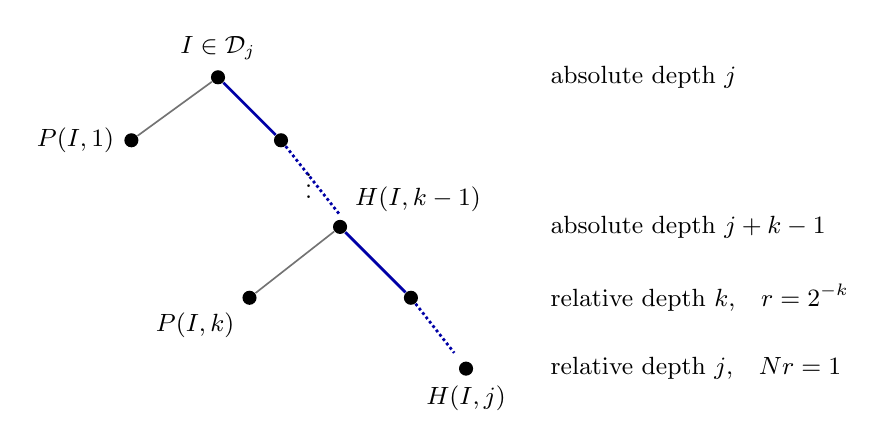
\begin{tikzpicture}[x=1cm,y=1cm,
  dot/.style={circle,fill=black,inner sep=1.8pt},
  heavy/.style={line width=1pt,blue!65!black},
  light/.style={line width=.6pt,black!55},
  every node/.style={font=\small}]
 \node[dot,label=above:{$I\in\mathcal D_j$}] (i) at (0,0) {};
 \node[dot] (h1) at (.8,-.8) {};
 \node[dot,label=left:{$P(I,1)$}] (l1) at (-1.1,-.8) {};
 \draw[heavy] (i)--(h1); \draw[light] (i)--(l1);
 \node at (1.15,-1.28) {$\vdots$};
 \draw[heavy,densely dotted] (h1)--(1.55,-1.75);
 \node[dot,label=above right:{$H(I,k-1)$}] (hk) at (1.55,-1.9) {};
 \node[dot,label=below left:{$P(I,k)$}] (lk) at (.4,-2.8) {};
 \node[dot] (hnext) at (2.45,-2.8) {};
 \draw[light] (hk)--(lk); \draw[heavy] (hk)--(hnext);
 \draw[heavy,densely dotted] (hnext)--(3,-3.5);
 \node[dot,label=below:{$H(I,j)$}] (end) at (3.15,-3.7) {};
 \node[anchor=west] at (4.1,0) {absolute depth $j$};
 \node[anchor=west] at (4.1,-1.9) {absolute depth $j+k-1$};
 \node[anchor=west] at (4.1,-2.8) {relative depth $k$,\quad $r=2^{-k}$};
 \node[anchor=west] at (4.1,-3.7) {relative depth $j$,\quad $Nr=1$};
\end{tikzpicture}

 \caption{A heavier-child path starting at absolute depth $j$.  Its
 lighter child at relative depth $k$ has a parent at absolute depth
 $j+k-1$.  Holding $k$ fixed and changing the frequency index $j$
 therefore selects distinct parent vertices in one common tree.
 The path stops at $k=j$, where the rescaled frequency is $Nr=1$.}
 \label{e:time-tree-figure}
\end{figure}

\Needspace{12\baselineskip}
\begin{theorem}[Local $L^1$ endpoint maximal estimate]
\label{e:maximal}
For compactly supported $\widehat f\in L^2$ and every unit ball $\Omega$,
\begin{equation}
 \int_\Omega\sup_{0\le t<1}|S(t)f(x)|\dd x
       \le C\norm{f}_{H^s(\R^n)}.
 \label{e:maximal-formula}
\end{equation}
The constant is uniform under translation of $\Omega$.
\end{theorem}

\begin{proof}
Take a smooth inhomogeneous Littlewood--Paley decomposition
$f=f_{\mathrm{lo}}+\sum_{j\ge1}f_{2^j}$ with bounded frequency overlap.
The low-frequency part satisfies
$\sup_{x,t}|S(t)f_{\mathrm{lo}}(x)|\le C\norm{f_{\mathrm{lo}}}_2$.
For a fixed measurable graph $t(x)$ and phase $w(x)$, frequency
Cauchy--Schwarz and \Cref{e:dual-square} give
\begin{align*}
 \left|\int_\Omega w(x)\sum_jS(t(x))f_{2^j}(x)\dd x\right|
 &\le C\left(\sum_j2^{2js}\norm{f_{2^j}}_2^2\right)^{1/2}
        \left(\sum_j2^{-2js}\norm{G_{2^j}([0,1))}_2^2\right)^{1/2}\\
 &\le C\norm{f}_{H^s}.
\end{align*}
Choose the annular cutoff in $G_{2^j}$ equal to one on the corresponding
Littlewood--Paley support.  The first factor is the Sobolev square sum;
no frequency logarithm or $\ell^1$ sum has appeared.
For a finite time list, select the first maximizer of the full field
and its conjugate phase (zero where the field is zero).  These are
measurable and are common to every frequency.  The preceding bound is
then the integral of that finite maximum.  Increase the lists to a
dense countable subset of $[0,1)$ containing zero.  Continuity of the
bounded-frequency field and monotone convergence prove
\eqref{e:maximal-formula}.  All kernel estimates depend only on spatial
differences, giving the asserted translation uniformity.
\end{proof}

\subsection{One representative and all real times}
\label{e:trace}

To complete \Cref{m:main}, we first construct a representative continuous
in time and then remove Gaussian regularization uniformly in time on
one full-measure spatial set.  The following approximate-identity lemma
will be applied to a countable family of error envelopes.

\begin{lemma}[Gaussian approximation with uniform local integrals]
\label{e:gaussian-local}
Let $M\ge0$ be measurable and
$A=\sup_z\int_{B(z,1)}M<\infty$.  For
\[
 K_a(y)=(4\pi a)^{-n/2}e^{-|y|^2/(4a)},\qquad a>0,
\]
the convolution $K_a*M$ is finite at every point.  At every Lebesgue
point $x$ of $M$, it tends to $M(x)$ as $a\downarrow0$.
\end{lemma}

\begin{proof}
For a fixed $\rho>0$, cover each annulus
$2^\ell\rho\le|y|<2^{\ell+1}\rho$ by
$C(1+2^\ell\rho)^n$ unit balls.  Uniformly in the center $x$,
\begin{equation}
 \int_{|y|\ge\rho}K_a(y)M(x-y)\dd y
 \le C A a^{-n/2}\sum_{\ell\ge0}(1+2^\ell\rho)^n
                    e^{-4^\ell\rho^2/(4a)}.
 \label{e:gaussian-annuli}
\end{equation}
The series is finite for every $a>0$, and for all sufficiently small
$a$ it is at most $C_\rho A a^{-n/2}e^{-\rho^2/(8a)}$.
The integral over a bounded ball is finite by local integrability,
which proves the first assertion.

At a Lebesgue point set
$H_x(r)=\int_{|y|<r}|M(x-y)-M(x)|\dd y=o(r^n)$.
Given $\eps>0$, choose $\rho$ so that $H_x(r)\le\eps r^n$ for
$0<r\le\rho$.  Radial integration by parts gives
\[
 \int_{|y|<\rho}K_a(y)|M(x-y)-M(x)|\dd y
 \le \eps\left(K_a(\rho)\rho^n+
                  \int_0^\rho(-K_a'(r))r^n\dd r\right)
 \le C\eps.
\]
The complementary integral tends to zero by
\eqref{e:gaussian-annuli}, together with the elementary Gaussian tail
bound for the constant $|M(x)|$.  Letting $\eps\downarrow0$ proves the
claim.
\end{proof}

\Needspace{8\baselineskip}
\begin{proof}[Proof of \Cref{m:main}]
Fix $n\ge3$ and a complex-valued $f\in H^s(\R^n)$.
Choose $f_j$ with $\widehat f_j\in C_c^\infty$ and
$\norm{f_j-f}_{H^s}\le2^{-j}$.  The successive differences satisfy a
summable $H^s$ bound.  By \Cref{e:maximal}, on every unit ball
\[
 \int\sum_j\sup_{0\le t<1}|S(t)(f_{j+1}-f_j)(x)|\dd x<\infty.
\]
A countable covering of $\R^n$ therefore gives a common full-measure
set $E_0$ on which $S(t)f_j(x)$ converges uniformly for $0\le t<1$.
Call the limit $v(x,t)$ and set $v(x,t)=0$ off $E_0$.  For every $x$,
$v(x,\cdot)$ is continuous on $[0,1)$; it is jointly measurable as a
pointwise limit on a measurable set.  The measurability of $E_0$ and of
all the suprema just used can equally be read from the countable dense
set of times, by continuity.

Fix an arbitrary real $t\in[0,1)$.  Unitarity gives
$S(t)f_j\to S(t)f$ in $L^2$, whereas the construction gives pointwise
convergence to $v(\cdot,t)$ almost everywhere.  Hence $v(\cdot,t)$ is
an $L^2$ representative of $S(t)f$.  For each $a>0$ and $x\in\R^n$,
the function $K_a(x-\cdot)$ lies in $L^2$.  Pairing it with this
$L^2$ class and using Plancherel yields the everywhere-defined identity
\begin{equation}
 U_a f(x,t)=(K_a*v(\cdot,t))(x).
 \label{e:class-gaussian-identity}
\end{equation}
The fixed $t$ was arbitrary.  Thus \eqref{e:class-gaussian-identity}
holds for every triple $(x,a,t)$ in the indicated ranges; no
intersection of time-dependent exceptional sets has been taken.
The convolution is absolutely convergent by Cauchy--Schwarz.

Let
\[
 M_j(x)=\sup_{0\le t<1}|v(x,t)-S(t)f_j(x)|.
\]
These functions are measurable because the supremum equals the one
over rational times.  They tend to zero on $E_0$.  Uniform convergence
there and Fatou's lemma applied to
$\sup_t|S(t)(f_\ell-f_j)|$ show that
\begin{equation}
 A_j:=\sup_z\int_{B(z,1)}M_j(x)\dd x
       \le C\norm{f-f_j}_{H^s}.
 \label{e:envelope-local-integrals}
\end{equation}
All translated balls have the same constant by \Cref{e:maximal}.
The values on the null complement of $E_0$ do not affect this estimate.
Intersect $E_0$ with the Lebesgue-point sets of the countably many
$M_j$.  By \Cref{e:gaussian-local}, at every point of this intersection
$K_a*M_j(x)\to M_j(x)$ for every $j$.

For every $y$ and every $t$, the definition of $M_j$ gives the
simultaneous inequality $|v(y,t)-S(t)f_j(y)|\le M_j(y)$.
Combining it with \eqref{e:class-gaussian-identity} gives
\begin{equation}
 \sup_{0<t<1}|U_a f(x,t)-v(x,t)|
 \le (K_a*M_j)(x)+M_j(x)+R_j(a),
 \label{e:envelope-gaussian-bound}
\end{equation}
where
\[
 R_j(a):=(2\pi)^{-n}
     \int |1-e^{-a|\xi|^2}|\,|\widehat f_j(\xi)|\dd\xi
       \longrightarrow0.
\]
This last convergence is uniform in $x,t$ since
$\widehat f_j\in L^1$.  First let $a\downarrow0$ at a point of the
common set.  The limsup of the left side of
\eqref{e:envelope-gaussian-bound} is at most $2M_j(x)$.
Then let $j\to\infty$.  This proves
\eqref{m:eq-uniform-Gaussian} for all real times in the interval
at once.

Finally, intersect with the Lebesgue points of $f$ and with the
full-measure set on which $v(x,0)=f(x)$, supplied by the fixed-time
$L^2$ identity at zero.  On the resulting $E_f$,
$v(x,0)=f^*(x)$ and time continuity gives
$v(x,t)\to f^*(x)$ as real $t\downarrow0$.
The Gaussian limit in \eqref{m:eq-uniform-Gaussian} is taken first,
so these are exactly the asserted iterated limits.
\end{proof}

\FloatBarrier
\phantomsection
\addcontentsline{toc}{section}{References}
\bibliographystyle{plainnat}
\bibliography{references}
\end{document}
